\documentclass[12pt, a4paper]{article}
\usepackage[utf8]{inputenc}
\usepackage{geometry}
\usepackage{graphicx}
\usepackage{multicol}
\usepackage{multirow}
\usepackage{tikz}
\usepackage{tabularx}
\usepackage{float}
\usepackage{array,booktabs,ragged2e}
\usepackage{amsmath}
\usepackage{siunitx}
\usepackage{physics}
\usepackage{xcolor}
\usepackage{wasysym}
\usepackage{ulem} %tallymarks
\usepackage{xkeyval}
\usepackage{tfrupee}
\graphicspath{{images/}}

\geometry{top=2.5cm, bottom=1.25cm, left=1.5cm, right=1.5cm}

% \pgfplotsset{compat=1.18}

\newtoks \coords 
\makeatletter

%%%%%%%%%%%%%%%%%%%%%%%%%%%%%%%%%%%  dimensions  %%%%%%%%%%%%%%%%%%%%%%%%%%%%%%%%%%%%%%%%%%%
\define@key{VerticalBar}{Width}{\def\VerticalBarwidth{#1}} % Width of Chart
\define@key{VerticalBar}{Height}{\def\VerticalBarheight{#1}}% Height of Chart
\define@key{VerticalBar}{Barwidth}{\def\VerticalBarbarwidth{#1}}% BarWidth of Chart
\define@key{VerticalBar}{Textwidth}{\def\VerticalBartextwidth{#1}}% Text width from axisline
\define@key{VerticalBar}{Scale}{\def\VerticalBarscale{#1}}% Size of Chart 
\define@key{VerticalBar}{YMax}{\def\VerticalBarYMax{#1}} % Y Axis Max Value
\define@key{VerticalBar}{YMin}{\def\VerticalBarYMin{#1}} % Y Axis Min Value

%%%%%%%%%%%%%%%%%%%%%%%%%%%%%%%%%%%%%% labels  %%%%%%%%%%%%%%%%%%%%%%%%%%%%%%%%%%%%%%%%%%%%%
\define@key{VerticalBar}{Xticklabels}{\def\VerticalBarXticklabels{#1}} % X axis Tick Labels 
\define@key{VerticalBar}{Ylabels}{\def\VerticalBarYlabels{#1}} % Y axis labels
\define@key{VerticalBar}{Xlabel}{\def\VerticalBarXlabel{#1}} % X axis label
\define@key{VerticalBar}{Xlabelrotate}{\def\VerticalBarXlabelrotate{#1}} % X tick label rotate

%%%%%%%%%%%%%%%%%%%%%%%%%%%%%%%%%%%%%% Axis Values  %%%%%%%%%%%%%%%%%%%%%%%%%%%%%%%%%%%%%%%%%%%%%
\define@key{VerticalBar}{Xtick}{\def\VerticalBarXtick{#1}}% X axis tick values
\define@key{VerticalBar}{Ytick}{\def\VerticalBarYtick{#1}}% Y axis tick values
\define@key{VerticalBar}{Barcoords}{\def\VerticalBarcoords{#1}}% Bar cordinates

%%%%%%%%%%%%%%%%%%%%%%%%%%%%%%%%%%%%%%%%%%%%%%%%%%%%%%%%%%%%%%%%%%%%%%%%%%%%%%%%%%%%%%%%%%%%%%%%

\define@key{VerticalBar}{Title}{\def\VerticalBartitle{#1}} % Title of Chart






\newcommand{\VerticalBar}[3]{
 \setkeys{VerticalBar}{#1}

\def \barcoords{\VerticalBarcoords}    

    \pgfmathsetmacro{\numOfBars}{{\barcoords}[0]}     
    \pgfmathsetmacro{\noOfCoords}{{\barcoords}[1]}     
    \centering
    \begin{tikzpicture}
    [scale=\VerticalBarscale]
                \begin{axis}[
                    width=\VerticalBarwidth cm,
                    height=\VerticalBarheight cm,
                    bar width=\VerticalBarbarwidth pt,
                    tick style={draw=none},
                    axis x line*=bottom,
                    axis y line*=left,
                    % Modified x-axis setup to show all labels
                    xtick=\VerticalBarXtick,
                    xtick distance=1,
                    x tick label as interval=false,
                    xticklabels/.expanded=\VerticalBarXticklabels,
                    xticklabel style={text width=\VerticalBartextwidth cm,align=center},
                    % ,rotate=10, anchor=east
                    ytick=\VerticalBarYtick,
                    ybar,
                    ymin=\VerticalBarYMin,
                    ymax=\VerticalBarYMax,
                    area legend,
                    ylabel={\VerticalBarYlabels},
                    xlabel={\VerticalBarXlabel},
                    nodes near coords,
                    nodes near coords style={font=\large},
                    nodes near coords align={vertical},
                    legend style={at={(0.5,-0.3)}, draw=none, anchor=north,legend columns=-1,column sep=0.2cm},
                    ymajorgrids=true,
                    title=\textbf{\VerticalBartitle},
                    % Ensure all x positions are shown
                    enlarge x limits={abs=0.5},
                    x tick label style={rotate=\VerticalBarXlabelrotate},
                ]

        \colorlet{Color1}{blue!30}
        \colorlet{Color2}{green!50}

        \foreach \i in {1,...,\numOfBars}{
            \coords{}
        
            \foreach \x in {0,...,\inteval{\noOfCoords-1}}{
                \pgfmathsetmacro{\eachpoint}{{\barcoords}[\i+1][\x]}
                \global\coords\expandafter{\expanded{\the\coords(\x+1,\eachpoint)}}
            }
            \edef \plotting{ \noexpand
                \addplot[ 
                    draw=none, 
                    fill=Color\i
                ] coordinates {
                    \the\coords
                }; \noexpand
            }
            
            \plotting

            \renewcommand{\coords}{{}}
        }
        \def\avg{#3} 
        \ifx\avg\empty{}
        \else
        {
            \draw[thick, dashed, color=red] (0,\avg) -- (\VerticalBarwidth,\avg);
        }
        \fi

        \legend{#2}
                \end{axis}
            \end{tikzpicture}
}


%-----------------------------------------------------------
     % text bottom 4 option in 1 row
%-----------------------------------------------------------

\define@key{mcqtextbottomFourOne}{questionnumber}{\def\mcqtextbottomFourOnequestionnumber{#1}} 
\define@key{mcqtextbottomFourOne}{questionTag}{\def\mcqtextbottomFourOnequestionTag{#1}}
\define@key{mcqtextbottomFourOne}{questiontext}{\def\mcqtextbottomFourOnequestiontext{#1}}
\define@key{mcqtextbottomFourOne}{optionA}{\def\mcqtextbottomFourOneoptionA{#1}}
\define@key{mcqtextbottomFourOne}{optionB}{\def\mcqtextbottomFourOneoptionB{#1}}
\define@key{mcqtextbottomFourOne}{optionC}{\def\mcqtextbottomFourOneoptionC{#1}}
\define@key{mcqtextbottomFourOne}{optionD}{\def\mcqtextbottomFourOneoptionD{#1}}
\define@key{mcqtextbottomFourOne}{correctoption}{\def\mcqtextbottomFourOnecorrectoption{#1}}


\newcommand{\mcqtextbottomFourOne}[1]{%
\setkeys{mcqtextbottomFourOne}{#1}%
\vspace{2.5mm}
\begin{raggedright}
\textbf{Question Tag:} \mcqtextbottomFourOnequestionTag \hfill \textbf{Correct Option:} \mcqtextbottomFourOnecorrectoption\\
\end{raggedright}
\vspace{\baselineskip}
\begin{raggedright}
\textbf{Question \mcqtextbottomFourOnequestionnumber:} \mcqtextbottomFourOnequestiontext\\
\medskip
(a) \medskip \mcqtextbottomFourOneoptionA\\
(b) \medskip \mcqtextbottomFourOneoptionB\\      
(c) \medskip \mcqtextbottomFourOneoptionC\\
(d) \medskip \mcqtextbottomFourOneoptionD\\
\end{raggedright}
}

%-----------------------------------------------------------

%-----------------------------------------------------------

% DEFINE KEY FOR mcqtextbottomOneFour %

\define@key{mcqtextbottomOneFour}{questionnumber}{\def\mcqtextbottomOneFourquestionnumber{#1}} 
\define@key{mcqtextbottomOneFour}{questiontext}{\def\mcqtextbottomOneFourquestiontext{#1}}
\define@key{mcqtextbottomOneFour}{optionA}{\def\mcqtextbottomOneFouroptionA{#1}}
\define@key{mcqtextbottomOneFour}{optionB}{\def\mcqtextbottomOneFouroptionB{#1}}
\define@key{mcqtextbottomOneFour}{optionC}{\def\mcqtextbottomOneFouroptionC{#1}}
\define@key{mcqtextbottomOneFour}{optionD}{\def\mcqtextbottomOneFouroptionD{#1}}
\define@key{mcqtextbottomOneFour}{questionTag}{\def\mcqtextbottomOneFourquestionTag{#1}} 
\define@key{mcqtextbottomOneFour}{correctoption}{\def\mcqtextbottomOneFourcorrectoption{#1}}
\define@key{mcqtextbottomOneFour}{coloredquestion}{\def\mcqtextbottomOneFourcolororblackwhite{#1}}

% COMMAND FOR mcqtextbottomOneFour %

\newcommand{\mcqtextbottomOneFour}[1]{%
\setkeys{mcqtextbottomOneFour}{#1}%
\vspace{2.5mm}
\begin{raggedright}
\textbf{Question Tag:} \mcqtextbottomOneFourquestionTag \hfill \textbf{Correct Option:} \mcqtextbottomOneFourcorrectoption\\
\end{raggedright}
\vspace{\baselineskip}
\begin{raggedright}
\textbf{Question \mcqtextbottomOneFourquestionnumber:} \mcqtextbottomOneFourquestiontext
\begin{multicols}{4}
(a) \medskip \mcqtextbottomOneFouroptionA\\
(b) \medskip \mcqtextbottomOneFouroptionB\\      
(c) \medskip \mcqtextbottomOneFouroptionC\\
(d) \medskip \mcqtextbottomOneFouroptionD\\
\end{multicols}
\end{raggedright}
}

%-----------------------------------------------------------

%-----------------------------------------------------------

% Define key FOR mcqtextbottomOneTwo 

\define@key{mcqtextbottomOneTwo}{questionnumber}{\def\mcqtextbottomOneTwoquestion{#1}}
\define@key{mcqtextbottomOneTwo}{questiontext}{\def\mcqtextbottomOneTwoquestiontext{#1}}
\define@key{mcqtextbottomOneTwo}{optionA}{\def\mcqtextbottomOneTwooptionA{#1}}
\define@key{mcqtextbottomOneTwo}{optionB}{\def\mcqtextbottomOneTwooptionB{#1}}
\define@key{mcqtextbottomOneTwo}{questionTag}{\def\mcqtextbottomOneTwoquestionTag{#1}}
\define@key{mcqtextbottomOneTwo}{correctoption}{\def\mcqtextbottomOneTwocorrectoption{#1}}

% COMMAND FOR mcqtextbottomOneTwo %

\newcommand{\mcqtextbottomOneTwo}[1]{%
\setkeys{mcqtextbottomOneTwo}{#1}%
\vspace{2.5mm}
\begin{raggedright}
\textbf{Question Tag:} \mcqtextbottomOneTwoquestionTag \hfill \textbf{Correct Option:} \mcqtextbottomOneTwocorrectoption\\
\end{raggedright}
\vspace{\baselineskip}
\begin{raggedright}
\textbf{Question \mcqtextbottomOneTwoquestion:} \mcqtextbottomOneTwoquestiontext\\
\begin{multicols}{2}
(a) \medskip \mcqtextbottomOneTwooptionA\\
(b) \medskip \mcqtextbottomOneTwooptionB\\
\end{multicols}
\end{raggedright}
}

%-----------------------------------------------------------

%-----------------------------------------------------------

% Define key FOR mcqtextbottomTwoTwo

\define@key{mcqtextbottomTwoTwo}{questionnumber}{\def\mcqtextbottomTwoTwoquestion{#1}}
\define@key{mcqtextbottomTwoTwo}{questiontext}{\def\mcqtextbottomTwoTwoquestiontext{#1}}
\define@key{mcqtextbottomTwoTwo}{optionA}{\def\mcqtextbottomTwoTwooptionA{#1}}
\define@key{mcqtextbottomTwoTwo}{optionB}{\def\mcqtextbottomTwoTwooptionB{#1}}
\define@key{mcqtextbottomTwoTwo}{optionC}{\def\mcqtextbottomTwoTwooptionC{#1}}
\define@key{mcqtextbottomTwoTwo}{optionD}{\def\mcqtextbottomTwoTwooptionD{#1}}
\define@key{mcqtextbottomTwoTwo}{questionTag}{\def\mcqtextbottomTwoTwoquestionTag{#1}}
\define@key{mcqtextbottomTwoTwo}{correctoption}{\def\mcqtextbottomTwoTwocorrectoption{#1}}

% COMMAND FOR mcqtextbottomTwoTwo %

\newcommand{\mcqtextbottomTwoTwo}[1]{%
\setkeys{mcqtextbottomTwoTwo}{#1}%
\vspace{1.5mm}
\begin{raggedright}
\textbf{Question Tag:} \mcqtextbottomTwoTwoquestionTag \hfill \textbf{Correct Option:} \mcqtextbottomTwoTwocorrectoption\\
\end{raggedright}
\vspace{\baselineskip}
\begin{raggedright}
\textbf{Question \mcqtextbottomTwoTwoquestion:} \mcqtextbottomTwoTwoquestiontext\\
\begin{multicols}{2}
(a) \medskip \mcqtextbottomTwoTwooptionA\\
(c) \medskip \mcqtextbottomTwoTwooptionC\\
\columnbreak
(b) \medskip \mcqtextbottomTwoTwooptionB\\
(d) \medskip \mcqtextbottomTwoTwooptionD\\
\end{multicols}
\end{raggedright}
\vspace{5mm}
}

%-----------------------------------------------------------

%-----------------------------------------------------------

% Define key FOR mcqtextsideFourOne


\define@key{mcqtextsideFourOne}{questionnumber}{\def\mcqtextsideFourOnequestionnumber{#1}} 
\define@key{mcqtextsideFourOne}{questionTag}{\def\mcqtextsideFourOnequestionTag{#1}} 
\define@key{mcqtextsideFourOne}{questiontext}{\def\mcqtextsideFourOnequestiontext{#1}}
\define@key{mcqtextsideFourOne}{optionA}{\def\mcqtextsideFourOneoptionA{#1}}
\define@key{mcqtextsideFourOne}{optionB}{\def\mcqtextsideFourOneoptionB{#1}}
\define@key{mcqtextsideFourOne}{optionC}{\def\mcqtextsideFourOneoptionC{#1}}
\define@key{mcqtextsideFourOne}{optionD}{\def\mcqtextsideFourOneoptionD{#1}}
\define@key{mcqtextsideFourOne}{correctoption}{\def\mcqtextsideFourOnecorrectoption{#1}}
\define@key{mcqtextsideFourOne}{leftmini}{\def\mcqtextsideFourOneleftmini{#1}}
\define@key{mcqtextsideFourOne}{rightmini}{\def\mcqtextsideFourOnerightmini{#1}}

% COMMAND FOR mcqtextsideFourOne

\newcommand{\mcqtextsideFourOne}[1]{%
\setkeys{mcqtextsideFourOne}{#1}%
\vspace{2.5mm}
\begin{raggedright}
\textbf{Question Tag:} \mcqtextsideFourOnequestionTag \hfill \textbf{Correct Option:} \mcqtextsideFourOnecorrectoption\\
\end{raggedright}
\vspace{\baselineskip}
\begin{raggedright}
\begin{minipage}[t]{\mcqtextsideFourOneleftmini\linewidth}
\textbf{Question \mcqtextsideFourOnequestionnumber:} \mcqtextsideFourOnequestiontext\\
\end{minipage}\hfill
\begin{minipage}[t]{\mcqtextsideFourOnerightmini\linewidth}
(a) \medskip \mcqtextsideFourOneoptionA\\
(b) \medskip \mcqtextsideFourOneoptionB\\
(c) \medskip \mcqtextsideFourOneoptionC\\
(d) \medskip \mcqtextsideFourOneoptionD\\
\end{minipage}
\end{raggedright}
}

%-----------------------------------------------------------

%-----------------------------------------------------------

% Define key FOR mcqimgbottomOneFour

\define@key{mcqimgbottomOneFour}{questionnumber}{\def\mcqimgbottomOneFourquestionnumber{#1}}
\define@key{mcqimgbottomOneFour}{questionTag}{\def\mcqimgbottomOneFourquestionTag{#1}}
\define@key{mcqimgbottomOneFour}{questiontext}{\def\mcqimgbottomOneFourquestiontext{#1}}
\define@key{mcqimgbottomOneFour}{optionA}{\def\mcqimgbottomOneFouroptionA{#1}}
\define@key{mcqimgbottomOneFour}{optionB}{\def\mcqimgbottomOneFouroptionB{#1}}
\define@key{mcqimgbottomOneFour}{optionC}{\def\mcqimgbottomOneFouroptionC{#1}}
\define@key{mcqimgbottomOneFour}{optionD}{\def\mcqimgbottomOneFouroptionD{#1}}
\define@key{mcqimgbottomOneFour}{correctoption}{\def\mcqimgbottomOneFourcorrectoption{#1}}

% COMMAND FOR mcqimgbottomOneFour %

\newcommand{\mcqimgbottomOneFour}[1]{%
\setkeys{mcqimgbottomOneFour}{#1}%
\vspace{2.5mm}
\begin{raggedright}
\textbf{Question Tag:} \mcqimgbottomOneFourquestionTag \hfill \textbf{Correct Option:} \mcqimgbottomOneFourcorrectoption\\
\end{raggedright}
\vspace{\baselineskip}
\begin{raggedright}
\textbf{Question \mcqimgbottomOneFourquestionnumber:} \mcqimgbottomOneFourquestiontext \\
\begin{multicols}{4}
(a) \includegraphics[width=\linewidth, height=3cm]{\mcqimgbottomOneFouroptionA}  \\
(b) \includegraphics[width=\linewidth, height=3cm]{\mcqimgbottomOneFouroptionB}   \\
(c) \includegraphics[width=\linewidth, height=3cm]{\mcqimgbottomOneFouroptionC}  \\
(d) \includegraphics[width=\linewidth, height=3cm]{\mcqimgbottomOneFouroptionD} 
\end{multicols}
\end{raggedright}
}

%-----------------------------------------------------------

%-----------------------------------------------------------

% Define key FOR mcqimgdbottomOneFour

\define@key{mcqimgdbottomOneFour}{questionnumber}{\def\mcqimgdbottomOneFourquestionnumber{#1}}
\define@key{mcqimgdbottomOneFour}{questionTag}{\def\mcqimgdbottomOneFourquestionTag{#1}}
\define@key{mcqimgdbottomOneFour}{questiontext}{\def\mcqimgdbottomOneFourquestiontext{#1}}
\define@key{mcqimgdbottomOneFour}{optionA}{\def\mcqimgdbottomOneFouroptionA{#1}}
\define@key{mcqimgdbottomOneFour}{optionAtext}{\def\mcqimgdbottomOneFouroptionAtext{#1}}
\define@key{mcqimgdbottomOneFour}{optionB}{\def\mcqimgdbottomOneFouroptionB{#1}}
\define@key{mcqimgdbottomOneFour}{optionBtext}{\def\mcqimgdbottomOneFouroptionBtext{#1}}
\define@key{mcqimgdbottomOneFour}{optionC}{\def\mcqimgdbottomOneFouroptionC{#1}}
\define@key{mcqimgdbottomOneFour}{optionCtext}{\def\mcqimgdbottomOneFouroptionCtext{#1}}
\define@key{mcqimgdbottomOneFour}{optionD}{\def\mcqimgdbottomOneFouroptionD{#1}}
\define@key{mcqimgdbottomOneFour}{optionDtext}{\def\mcqimgdbottomOneFouroptionDtext{#1}}
\define@key{mcqimgdbottomOneFour}{correctoption}{\def\mcqimgdbottomOneFourcorrectoption{#1}}

% COMMAND FOR mcqimgdbottomOneFour %

\newcommand{\mcqimgdbottomOneFour}[1]{%
\setkeys{mcqimgdbottomOneFour}{#1}%
\vspace{2.5mm}
\begin{raggedright}
\textbf{Question Tag:} \mcqimgdbottomOneFourquestionTag \hfill \textbf{Correct Option:} \mcqimgdbottomOneFourcorrectoption\\
\end{raggedright}
\vspace{\baselineskip}
\begin{raggedright}
\textbf{Question \mcqimgdbottomOneFourquestionnumber:} \mcqimgdbottomOneFourquestiontext \\
\begin{multicols}{4}
\includegraphics[width=\linewidth, height=3cm]{\mcqimgdbottomOneFouroptionA} 
(a) \mcqimgdbottomOneFouroptionAtext \\

\includegraphics[width=\linewidth, height=3cm]{\mcqimgdbottomOneFouroptionB}       
(b) \mcqimgdbottomOneFouroptionBtext \\

\includegraphics[width=\linewidth, height=3cm]{\mcqimgdbottomOneFouroptionC} 
(c) \mcqimgdbottomOneFouroptionCtext \\

\includegraphics[width=\linewidth, height=3cm]{\mcqimgdbottomOneFouroptionD} 
(d) \mcqimgdbottomOneFouroptionDtext
\end{multicols}
\end{raggedright}
}

%-----------------------------------------------------------

%-----------------------------------------------------------

% Define key FOR mcqimgleftFourOne

\define@key{mcqimgleftFourOne}{questionnumber}{\def\mcqimgleftFourOnequestionnumber{#1}} 
\define@key{mcqimgleftFourOne}{questiontext}{\def\mcqimgleftFourOnequestiontext{#1}}
\define@key{mcqimgleftFourOne}{imgtabletikz}{\def\mcqimgtabletikz{#1}}
\define@key{mcqimgleftFourOne}{optionA}{\def\mcqimgleftFourOneoptionA{#1}}
\define@key{mcqimgleftFourOne}{optionB}{\def\mcqimgleftFourOneoptionB{#1}}
\define@key{mcqimgleftFourOne}{optionC}{\def\mcqimgleftFourOneoptionC{#1}}
\define@key{mcqimgleftFourOne}{optionD}{\def\mcqimgleftFourOneoptionD{#1}}
\define@key{mcqimgleftFourOne}{questionTag}{\def\mcqimgleftFourOnequestionTag{#1}} 
\define@key{mcqimgleftFourOne}{correctoption}{\def\mcqimgleftFourOnecorrectoption{#1}}
\define@key{mcqimgleftFourOne}{leftmini}{\def\mcqimgleftFourOneleftmini{#1}}
\define@key{mcqimgleftFourOne}{rightmini}{\def\mcqimgleftFourOnerightmini{#1}}

% COMMAND FOR mcqimgleftFourOne 

\newcommand{\mcqimgleftFourOne}[1]{%
\setkeys{mcqimgleftFourOne}{#1}%
\vspace{1.5mm}
\begin{raggedright}
\textbf{Question Tag:} \mcqimgleftFourOnequestionTag \hfill \textbf{Correct Option:} \mcqimgleftFourOnecorrectoption\\
\end{raggedright}
\vspace{\baselineskip}
\begin{raggedright}
\textbf{Question \mcqimgleftFourOnequestionnumber:} \mcqimgleftFourOnequestiontext\\
\medskip
\end{raggedright}
\begin{minipage}[]{\mcqimgleftFourOneleftmini\linewidth}
\Centering
\mcqimgtabletikz 
\end{minipage}\hfill
\begin{minipage}[]{\mcqimgleftFourOnerightmini\linewidth}
(a) \medskip \mcqimgleftFourOneoptionA\\
(b) \medskip \mcqimgleftFourOneoptionB\\
(c) \medskip \mcqimgleftFourOneoptionC\\
(d) \medskip \mcqimgleftFourOneoptionD\\      
\end{minipage}
\vspace{3mm}
}

%-----------------------------------------------------------

%-----------------------------------------------------------

% DEFINE KEY FOR mcqfourimg %

\define@key{mcqimgsideFourOne}{questionnumber} {\def\mcqimgsideFourOnequestionnumber{#1} }
\define@key{mcqimgsideFourOne}{questiontext}{\def\mcqimgsideFourOnequestiontext{#1}}
\define@key{mcqimgsideFourOne}{imgwidth}{\def\mcqimgsideFourOnewidth{#1}}
\define@key{mcqimgsideFourOne}{imgheight}{\def\mcqimgsideFourOneheight{#1}}
\define@key{mcqimgsideFourOne}{img}{\def\mcqimgsideFourOne{#1}}
\define@key{mcqimgsideFourOne}{optionA}{\def\mcqimgsideFourOneoptionA{#1}}
\define@key{mcqimgsideFourOne}{optionB}{\def\mcqimgsideFourOneoptionB{#1}}
\define@key{mcqimgsideFourOne}{optionC}{\def\mcqimgsideFourOneoptionC{#1}}
\define@key{mcqimgsideFourOne}{optionD}{\def\mcqimgsideFourOneoptionD{#1}}
\define@key{mcqimgsideFourOne}{questionTag}{\def\mcqimgsideFourOnequestionTag{#1}} 
\define@key{mcqimgsideFourOne}{correctoption}{\def\mcqimgsideFourOnecorrectoption{#1}}
\define@key{mcqimgsideFourOne}{leftmini}{\def\mcqimgsideFourOneleftmini{#1}}
\define@key{mcqimgsideFourOne}{rightmini}{\def\mcqimgsideFourOnerightmini{#1}}

\newcommand{\mcqimgsideFourOne}[1]{
\setkeys{mcqimgsideFourOne}{#1}
\vspace{2.5mm}
\begin{raggedright}
\textbf{Question Tag:} \mcqimgsideFourOnequestionTag \hfill \textbf{Correct Option:} \mcqimgsideFourOnecorrectoption \\
\end{raggedright}
\vspace{\baselineskip}
\begin{raggedright}
\begin{minipage}[]{\mcqimgsideFourOneleftmini\textwidth}
\textbf{Question \mcqimgsideFourOnequestionnumber:} \mcqimgsideFourOnequestiontext
\vspace{2mm} \\
(a) \medskip \mcqimgsideFourOneoptionA \\
(b) \medskip \mcqimgsideFourOneoptionB \\
(c) \medskip \mcqimgsideFourOneoptionC \\
(d) \medskip \mcqimgsideFourOneoptionD \\
\end{minipage}
\begin{minipage}[]{\mcqimgsideFourOnerightmini\textwidth}
\includegraphics[width=\mcqimgsideFourOnewidth, height=\mcqimgsideFourOneheight]{\mcqimgsideFourOne}
\end{minipage}
\end{raggedright}
\vspace{5mm}
 }

%-----------------------------------------------------------
%               MCQ without Option
%-----------------------------------------------------------


\define@key{mcqdescriptive}{questionnumber}{\def\mcqdescriptivequestionnumber{#1}} 
\define@key{mcqdescriptive}{questionTag}{\def\mcqdescriptivequestionTag{#1}} 
\define@key{mcqdescriptive}{questiontext}{\def\mcqdescriptivequestiontext{#1}}
\define@key{mcqdescriptive}{correctoption}{\def\mcqdescriptivecorrectoption{#1}}

\newcommand{\mcqdescriptive}[1]{%
\setkeys{mcqdescriptive}{#1}%
\vspace{2.5mm}
\begin{raggedright}
\textbf{Question Tag:} \mcqdescriptivequestionTag \hfill \textbf{Correct Option:} \mcqdescriptivecorrectoption\\
\end{raggedright}
\vspace{\baselineskip}
\begin{raggedright}
\textbf{Question \mcqdescriptivequestionnumber:} \mcqdescriptivequestiontext
\end{raggedright}
\vspace{5mm}}


%-----------------------------------------------------------
%                        TABLE
%-----------------------------------------------------------
\newcolumntype{R}[1]{>{\Centering\arraybackslash}p{#1}}
\makeatother

%-----------------------------------------------------------
%                        Start Question
%-----------------------------------------------------------
\begin{document}

%-----------------------------------------------------------
%                        Question [ 1 ]
%-----------------------------------------------------------
% start-of-question
\mcqtextbottomOneFour{
questionnumber={1}, 
questiontext={Find the missing place in the given place value table. \\
\medskip
\renewcommand{\arraystretch}{1.25}
\begin{tabular}{|>{\centering\arraybackslash}p{3cm}|p{3cm}|>{\centering\arraybackslash}p{3cm}|>{\centering\arraybackslash}p{3cm}|>{\centering\arraybackslash}p{3cm}|}
\hline
Ten thousands & \Centering{?} & Hundreds & Tens & Ones \\
\hline
\end{tabular} },
optionA={Ten lakhs},
optionB={Ten thousand},
optionC={Ones},
optionD={Thousands},
questionTag={C6M01 - DT - Q1}, 
correctoption={D},
}
% end-of-question

%-----------------------------------------------------------
%                        Question [ 2 ]
%-----------------------------------------------------------
% start-of-question
\mcqtextbottomOneFour{
questionnumber={2}, 
questiontext={Find the missing number. (Hint: Using place values)\\
\hspace{3cm} 8190 = 8000 + \rule{50pt}{0.5pt} +  90},
optionA={1},
optionB={10},
optionC={100},
optionD={190},
questionTag={C6M01 - DT - Q2}, 
correctoption={C},
}
% end-of-question

%-----------------------------------------------------------
%                        Question [ 3 ]
%-----------------------------------------------------------
% start-of-question
\mcqtextbottomOneFour{
questionnumber={3}, 
questiontext={In 231056, find the number that represents lakhs.},
optionA={2},
optionB={5},
optionC={3},
optionD={0},
questionTag={C6M01 - DT - Q3}, 
correctoption={A},
}
% end-of-question

%-----------------------------------------------------------
%                        Question [ 4 ]
%-----------------------------------------------------------
% start-of-question
\mcqtextbottomOneFour{
questionnumber={4}, 
questiontext={Count the number of digits in the given large number. \quad  98765432},
optionA={9},
optionB={8},
optionC={7},
optionD={4},
questionTag={C6M01 - DT - Q4}, 
correctoption={B},
}
% end-of-question


%-----------------------------------------------------------
%                        Question [ 5 ]
%-----------------------------------------------------------
% start-of-question
\mcqimgleftFourOne{
questionnumber={5}, 
questiontext={Compare.},
imgtabletikz = { 
\tikzset{every picture/.style={line width=0.75pt}} 
\begin{tikzpicture}[x=0.75pt,y=0.75pt,yscale=-1,xscale=1]
\draw (158.5,90.5) node  {
\includegraphics[width=74.25pt,height=55pt]{C6M01 - DT - Q5i.png}};
\draw (354.5,89.5) node  {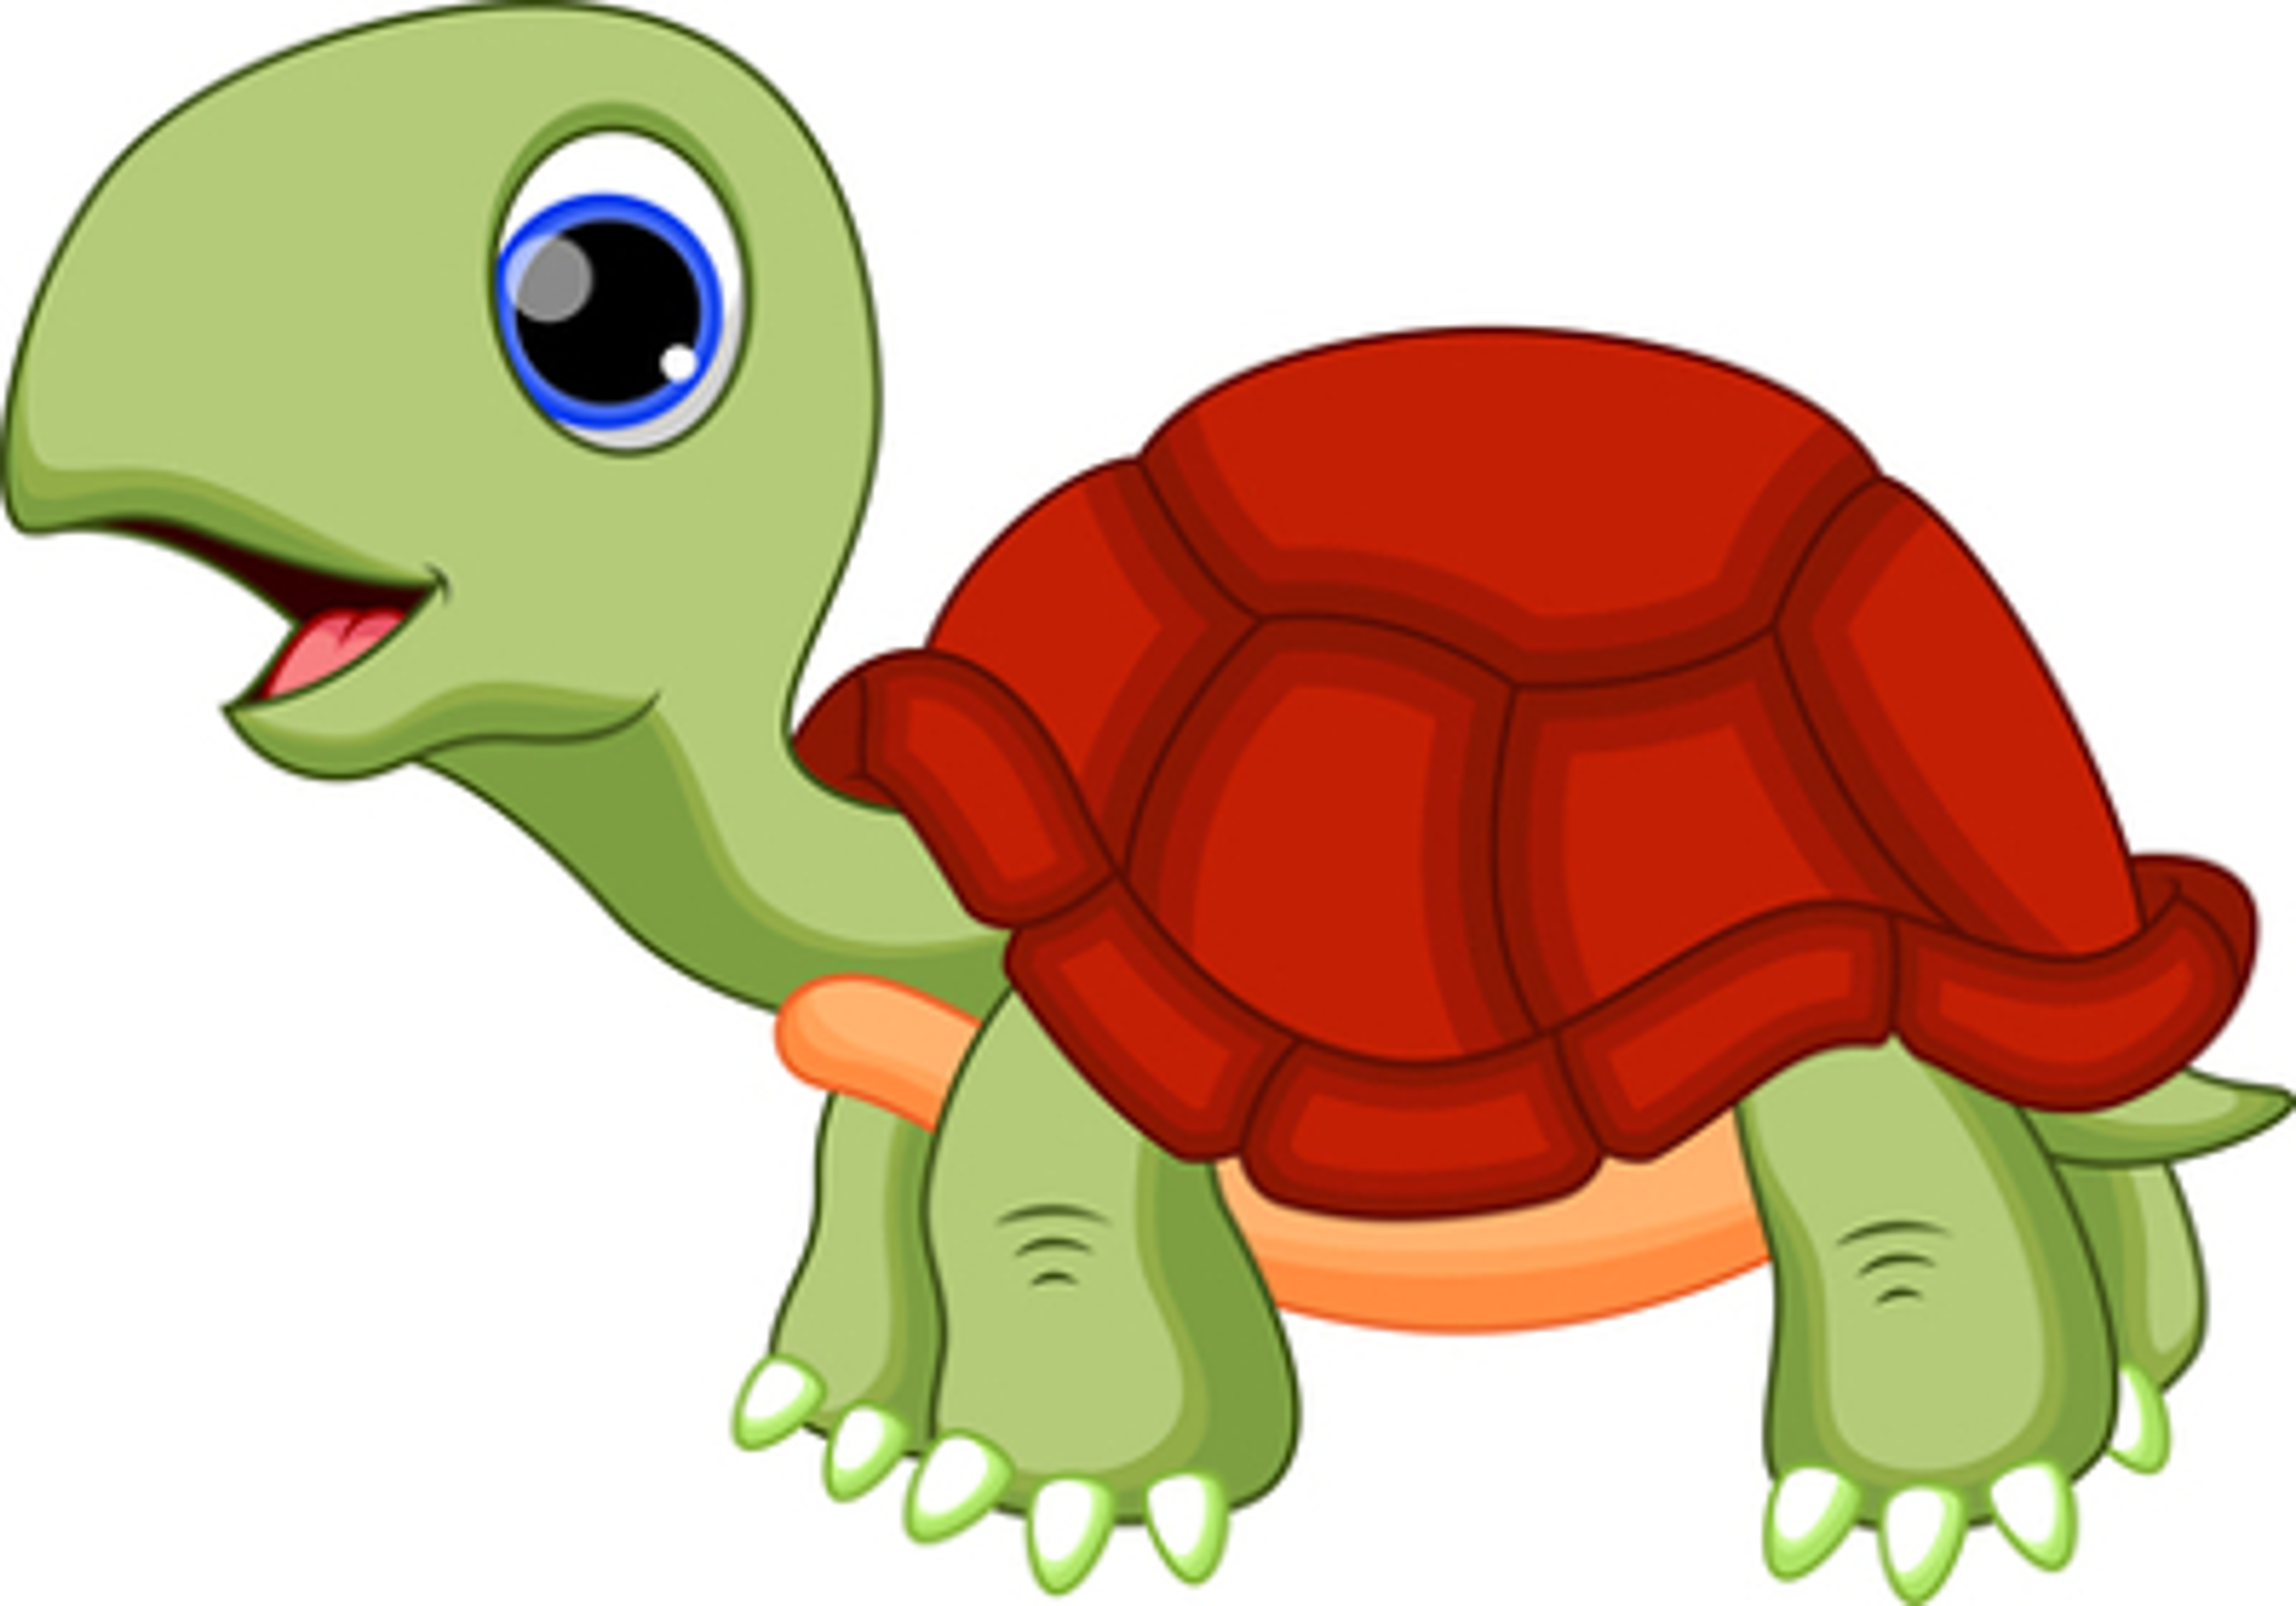
\includegraphics[width=74.25pt,height=55pt]{C6M01 - DT - Q5ii.png}};
\draw   (243,76) -- (276,76) -- (276,109) -- (243,109) -- cycle ;
\draw (88,133) node [anchor=north west][inner sep=0.75pt]   [align=left] {150000 green tortoise};
\draw (294,133) node [anchor=north west][inner sep=0.75pt]   [align=left] {130000 red tortoise};
\end{tikzpicture} },
optionA={$<$},
optionB={$>$},
optionC={$=$},
optionD={None of the above},
questionTag={C6M01 - DT - Q5}, 
leftmini={0.5},
rightmini={0.4},
correctoption={B},
}
% end-of-question

%-----------------------------------------------------------
%                        Question [ 6 ]
%-----------------------------------------------------------
% start-of-question
\mcqimgleftFourOne{
questionnumber={6}, 
questiontext={Add. },
imgtabletikz  = {  
\renewcommand{\arraystretch}{1.5}
\begin{tabular}{cccccc}
  & 8 & 2 & 5 & 7 & 0  \\
 + & 5 & 8 & 3 & 2 & 0 \\
 \hline
 &&&&&\\
 \hline
\end{tabular} },
optionA={1310890},
optionB={140980},
optionC={140890},
optionD={14890},
questionTag={C6M01 - DT - Q6},
leftmini={0.5},
rightmini={0.4},
correctoption={C},
}
% end-of-question

%-----------------------------------------------------------
%                        Question [ 7 ]
%-----------------------------------------------------------
% start-of-question
\mcqtextbottomOneFour{
questionnumber={7}, 
questiontext={Find the remainder of the following. \quad 19477 $\divisionsymbol$ 9 },
optionA={1},
optionB={0},
optionC={2164},
optionD={2184},
questionTag={C6M01 - DT - Q7}, 
correctoption={A},
}
% end-of-question

%-----------------------------------------------------------
%                        Question [ 8 ]
%-----------------------------------------------------------
% start-of-question
\mcqtextbottomOneFour{
questionnumber={8}, 
questiontext={1 centimetre is equal to \rule{40pt}{0.5pt} mm.},
optionA={100 mm},
optionB={1000 cm},
optionC={0.1 mm},
optionD={10 mm},
questionTag={C6M01 - DT - Q8}, 
correctoption={D},
}
% end-of-question

%-----------------------------------------------------------
%                        Question [ 9 ]
%-----------------------------------------------------------
% start-of-question
\mcqimgleftFourOne{
questionnumber={9}, 
questiontext={Match the following.},
imgtabletikz  = { 
\renewcommand{\arraystretch}{1.25}
\begin{tabular}{|p{0.5cm}|p{4cm}|p{0.5cm}|p{0.5cm}|p{3cm}|}
\cline{1-2}\cline{4-5} 
\multicolumn{2}{|c|}{\textbf{Column A}} & 
\multirow{4}[10]{*}{} &   
\multicolumn{2}{c|}{\textbf{Column B}} \\
\cline{1-2}\cline{4-5} i & 10 m in cm &   & a & 1000\\
\cline{1-2}\cline{4-5} ii & 10000 m in km &   & b & 100 \\
\cline{1-2}\cline{4-5} iii & 1000 mm in cm &   & c & 10 \\
\cline{1-2}\cline{4-5}
\end{tabular} },
optionA={i - c, ii - b, iii - a},
optionB={i - a, ii - c, iii - b},
optionC={i - a, ii - b, iii - c},
optionD={i - b, ii - c, iii - a},
questionTag={C6M01 - DT - Q9}, 
correctoption={B},
leftmini={0.7},
rightmini={0.3}
}
% end-of-question

%-----------------------------------------------------------
%                        Question [ 10 ]
%-----------------------------------------------------------
% start-of-question
\mcqtextbottomOneFour{
questionnumber={10}, 
questiontext={Round off the given number to the nearest thousand place. \quad 1200},
optionA={1000},
optionB={1500},
optionC={900},
optionD={2000},
questionTag={C6M01 - DT - Q10}, 
correctoption={A},
}
% end-of-question

%-----------------------------------------------------------
%                        Question [ 11 ]
%-----------------------------------------------------------
% start-of-question
\mcqtextbottomOneFour{
questionnumber={11}, 
questiontext={Estimate: 19 $\times$ 78},
optionA={1480},
optionB={1500},
optionC={1600},
optionD={400},
questionTag={C6M01 - DT - Q11}, 
correctoption={C},
}
% end-of-question

%-----------------------------------------------------------
%                        Question [  ]
%-----------------------------------------------------------
% start-of-question
\mcqtextbottomOneFour{
questionnumber={12}, 
questiontext={Find the number that represents ten thousand. \quad		9756563},
optionA={6},
optionB={5},
optionC={7},
optionD={9},
questionTag={C6M01 - DT - Q12}, 
correctoption={B},
}
% end-of-question

%-----------------------------------------------------------
%                        Question [ 3 ]
%-----------------------------------------------------------
% start-of-question
\mcqtextbottomTwoTwo{
questionnumber={13}, 
questiontext={Express the number in words: 220040},
optionA={Twenty-two thousand and forty},
optionB={Twenty-two hundred and forty},
optionC={Two lakh two hundred and forty},
optionD={Two lakh twenty thousand and forty},
questionTag={C6M01 - DT - Q13}, 
correctoption={D},
}
% end-of-question


%-----------------------------------------------------------
%                        Question [ 12 ]
%-----------------------------------------------------------
% start-of-question
\mcqimgleftFourOne{ 
questionnumber={1}, 
questiontext={Which flag does not contain a natural number?},
imgtabletikz = { 
\includegraphics[width=10cm, height=2.5cm]{C6M03 - DT - Q1.png}},
optionA={Green},
optionB={Blue},
optionC={Orange},
optionD={Red},
questionTag={C6M03 - DT - Q1}, 
correctoption={B},
leftmini={0.5},
rightmini={0.3},
}
% end-of-question

%-----------------------------------------------------------
%                        Question [ 13 ]
%-----------------------------------------------------------
% start-of-question
\mcqtextbottomOneFour{
questionnumber={2}, 
questiontext={Multiply.\\
\qquad i.   10 $\times$ 9 = \rule{50pt}{0.5pt}\\
\qquad ii.  12 $\times$ 19 = \rule{50pt}{0.5pt}},
optionA={ 90, 120},
optionB={90, 228},
optionC={109, 120 },
optionD={109, 228},
questionTag={C6M03 - DT - Q2}, 
correctoption={B},
}
% end-of-question


%-----------------------------------------------------------
%                        Question [ 14 ]
%-----------------------------------------------------------
% start-of-question
\mcqtextbottomTwoTwo{
questionnumber={3}, 
questiontext={Which of the following number lines shows 3 × 2?},
optionA={
\tikzset{every picture/.style={line width=0.75pt}} 
\begin{tikzpicture}[x=0.75pt,y=0.75pt,yscale=-0.75,xscale=0.75]
\draw    (201.35,101.01) -- (540,101.99) (239.37,92.62) -- (239.33,109.62)(277.37,92.73) -- (277.32,109.73)(315.37,92.84) -- (315.32,109.84)(353.37,92.95) -- (353.32,109.95)(391.37,93.06) -- (391.32,110.06)(429.37,93.17) -- (429.32,110.17)(467.37,93.28) -- (467.32,110.28)(505.37,93.39) -- (505.32,110.39) ;
\draw [shift={(543,102)}, rotate = 180.17] [fill={rgb, 255:red, 0; green, 0; blue, 0 }  ][line width=0.08]  [draw opacity=0] (10.72,-5.15) -- (0,0) -- (10.72,5.15) -- (7.12,0) -- cycle    ;
\draw [shift={(199,101)}, rotate = 0.17] [color={rgb, 255:red, 0; green, 0; blue, 0 }  ][line width=0.75]      (0, 0) circle [x radius= 3.35, y radius= 3.35]   ;
\draw  [draw opacity=0][dash pattern={on 4.5pt off 4.5pt}] (238,93.23) .. controls (240.77,69.79) and (266.23,51.69) .. (296.94,52.14) .. controls (327.57,52.59) and (352.42,71.33) .. (354.58,94.76) -- (296.24,97.77) -- cycle ; \draw [dash pattern={on 4.5pt off 4.5pt}] [dash pattern={on 4.5pt off 4.5pt}]  (238,93.23) .. controls (240.77,69.79) and (266.23,51.69) .. (296.94,52.14) .. controls (327.57,52.59) and (352.42,71.33) .. (354.58,94.76) ; \draw [shift={(354.58,94.76)}, rotate = 83.06] [color={rgb, 255:red, 0; green, 0; blue, 0 }  ][fill={rgb, 255:red, 0; green, 0; blue, 0 }  ][dash pattern={on 4.5pt off 4.5pt}][line width=0.75]      (0, 0) circle [x radius= 3.35, y radius= 3.35]   ; 
\draw  [draw opacity=0][dash pattern={on 4.5pt off 4.5pt}] (352.43,95.57) .. controls (353.83,71.25) and (370.71,52.15) .. (391.02,52.44) .. controls (411.3,52.74) and (427.57,72.27) .. (428.28,96.56) -- (390.32,98.53) -- cycle ; \draw [dash pattern={on 4.5pt off 4.5pt}] [dash pattern={on 4.5pt off 4.5pt}]  (352.43,95.57) .. controls (353.83,71.25) and (370.71,52.15) .. (391.02,52.44) .. controls (410.79,52.73) and (426.75,71.3) .. (428.19,94.75) ; \draw [shift={(428.28,96.56)}, rotate = 266.86] [color={rgb, 255:red, 0; green, 0; blue, 0 }  ][dash pattern={on 4.5pt off 4.5pt}][line width=0.75]    (10.93,-4.9) .. controls (6.95,-2.3) and (3.31,-0.67) .. (0,0) .. controls (3.31,0.67) and (6.95,2.3) .. (10.93,4.9)   ; 
\draw (348,116) node [anchor=north west][inner sep=0.75pt]   [align=left] {3};
\draw (272,115) node [anchor=north west][inner sep=0.75pt]   [align=left] {1};
\draw (308,116) node [anchor=north west][inner sep=0.75pt]   [align=left] {2};
\draw (232,115) node [anchor=north west][inner sep=0.75pt]   [align=left] {0};
\draw (386,117) node [anchor=north west][inner sep=0.75pt]   [align=left] {4};
\draw (423,116) node [anchor=north west][inner sep=0.75pt]   [align=left] {5};
\draw (461,115) node [anchor=north west][inner sep=0.75pt]   [align=left] {6};
\draw (499,116) node [anchor=north west][inner sep=0.75pt]   [align=left] {7};
\end{tikzpicture} },
optionB={
\tikzset{every picture/.style={line width=0.75pt}} 
\begin{tikzpicture}[x=0.75pt,y=0.75pt,yscale=-0.75,xscale=0.75]
\draw    (221.35,121.01) -- (560,121.99) (259.37,112.62) -- (259.33,129.62)(297.37,112.73) -- (297.32,129.73)(335.37,112.84) -- (335.32,129.84)(373.37,112.95) -- (373.32,129.95)(411.37,113.06) -- (411.32,130.06)(449.37,113.17) -- (449.32,130.17)(487.37,113.28) -- (487.32,130.28)(525.37,113.39) -- (525.32,130.39) ;
\draw [shift={(563,122)}, rotate = 180.17] [fill={rgb, 255:red, 0; green, 0; blue, 0 }  ][line width=0.08]  [draw opacity=0] (10.72,-5.15) -- (0,0) -- (10.72,5.15) -- (7.12,0) -- cycle    ;
\draw [shift={(219,121)}, rotate = 0.17] [color={rgb, 255:red, 0; green, 0; blue, 0 }  ][line width=0.75]      (0, 0) circle [x radius= 3.35, y radius= 3.35]   ;
\draw  [draw opacity=0][dash pattern={on 4.5pt off 4.5pt}] (257.87,113.11) .. controls (259.35,89.81) and (276.62,71.55) .. (297.41,71.86) .. controls (318.16,72.16) and (334.84,90.86) .. (335.65,114.13) -- (296.73,116.14) -- cycle ; \draw [dash pattern={on 4.5pt off 4.5pt}] [dash pattern={on 4.5pt off 4.5pt}]  (257.87,113.11) .. controls (259.35,89.81) and (276.62,71.55) .. (297.41,71.86) .. controls (318.16,72.16) and (334.84,90.86) .. (335.65,114.13) ; \draw [shift={(335.65,114.13)}, rotate = 86.41] [color={rgb, 255:red, 0; green, 0; blue, 0 }  ][fill={rgb, 255:red, 0; green, 0; blue, 0 }  ][dash pattern={on 4.5pt off 4.5pt}][line width=0.75]      (0, 0) circle [x radius= 3.35, y radius= 3.35]   ; 
\draw  [draw opacity=0][dash pattern={on 4.5pt off 4.5pt}] (335.91,111.12) .. controls (338.6,88.89) and (363.11,71.74) .. (392.67,72.17) .. controls (422.15,72.61) and (446.07,90.38) .. (448.19,112.59) -- (392,115.5) -- cycle ; \draw [dash pattern={on 4.5pt off 4.5pt}] [dash pattern={on 4.5pt off 4.5pt}]  (335.91,111.12) .. controls (338.6,88.89) and (363.11,71.74) .. (392.67,72.17) .. controls (421.41,72.6) and (444.87,89.5) .. (447.99,110.94) ; \draw [shift={(448.19,112.59)}, rotate = 262.86] [color={rgb, 255:red, 0; green, 0; blue, 0 }  ][dash pattern={on 4.5pt off 4.5pt}][line width=0.75]    (10.93,-4.9) .. controls (6.95,-2.3) and (3.31,-0.67) .. (0,0) .. controls (3.31,0.67) and (6.95,2.3) .. (10.93,4.9)   ; 
\draw (368,136) node [anchor=north west][inner sep=0.75pt]   [align=left] {3};
\draw (292,135) node [anchor=north west][inner sep=0.75pt]   [align=left] {1};
\draw (328,136) node [anchor=north west][inner sep=0.75pt]   [align=left] {2};
\draw (252,135) node [anchor=north west][inner sep=0.75pt]   [align=left] {0};
\draw (406,137) node [anchor=north west][inner sep=0.75pt]   [align=left] {4};
\draw (443,136) node [anchor=north west][inner sep=0.75pt]   [align=left] {5};
\draw (481,135) node [anchor=north west][inner sep=0.75pt]   [align=left] {6};
\draw (519,136) node [anchor=north west][inner sep=0.75pt]   [align=left] {7};
\end{tikzpicture} },
optionC={
\tikzset{every picture/.style={line width=0.75pt}} 
\begin{tikzpicture}[x=0.75pt,y=0.75pt,yscale=-0.75,xscale=0.75]
\draw    (152.35,124.01) -- (491,124.99) (190.37,115.62) -- (190.33,132.62)(228.37,115.73) -- (228.32,132.73)(266.37,115.84) -- (266.32,132.84)(304.37,115.95) -- (304.32,132.95)(342.37,116.06) -- (342.32,133.06)(380.37,116.17) -- (380.32,133.17)(418.37,116.28) -- (418.32,133.28)(456.37,116.39) -- (456.32,133.39) ;
\draw [shift={(494,125)}, rotate = 180.17] [fill={rgb, 255:red, 0; green, 0; blue, 0 }  ][line width=0.08]  [draw opacity=0] (10.72,-5.15) -- (0,0) -- (10.72,5.15) -- (7.12,0) -- cycle    ;
\draw [shift={(150,124)}, rotate = 0.17] [color={rgb, 255:red, 0; green, 0; blue, 0 }  ][line width=0.75]      (0, 0) circle [x radius= 3.35, y radius= 3.35]   ;
\draw  [draw opacity=0][dash pattern={on 4.5pt off 4.5pt}] (188.87,116.11) .. controls (190.35,92.81) and (207.62,74.55) .. (228.41,74.86) .. controls (249.16,75.16) and (265.84,93.86) .. (266.65,117.13) -- (227.73,119.14) -- cycle ; \draw [dash pattern={on 4.5pt off 4.5pt}] [dash pattern={on 4.5pt off 4.5pt}]  (188.87,116.11) .. controls (190.35,92.81) and (207.62,74.55) .. (228.41,74.86) .. controls (249.16,75.16) and (265.84,93.86) .. (266.65,117.13) ; \draw [shift={(266.65,117.13)}, rotate = 86.41] [color={rgb, 255:red, 0; green, 0; blue, 0 }  ][fill={rgb, 255:red, 0; green, 0; blue, 0 }  ][dash pattern={on 4.5pt off 4.5pt}][line width=0.75]      (0, 0) circle [x radius= 3.35, y radius= 3.35]   ;
\draw  [draw opacity=0][dash pattern={on 4.5pt off 4.5pt}] (266.65,117.13) .. controls (268.14,93.83) and (285.4,75.57) .. (306.19,75.87) .. controls (326.94,76.18) and (343.62,94.87) .. (344.44,118.15) -- (305.51,120.16) -- cycle ; \draw [dash pattern={on 4.5pt off 4.5pt}] [dash pattern={on 4.5pt off 4.5pt}]  (266.65,117.13) .. controls (268.14,93.83) and (285.4,75.57) .. (306.19,75.87) .. controls (326.94,76.18) and (343.62,94.87) .. (344.44,118.15) ; \draw [shift={(344.44,118.15)}, rotate = 86.41] [color={rgb, 255:red, 0; green, 0; blue, 0 }  ][fill={rgb, 255:red, 0; green, 0; blue, 0 }  ][dash pattern={on 4.5pt off 4.5pt}][line width=0.75]      (0, 0) circle [x radius= 3.35, y radius= 3.35]   ;
\draw  [draw opacity=0][dash pattern={on 4.5pt off 4.5pt}] (344.44,118.15) .. controls (345.92,94.85) and (363.19,76.59) .. (383.97,76.89) .. controls (404.72,77.2) and (421.4,95.89) .. (422.22,119.17) -- (383.29,121.18) -- cycle ; \draw [dash pattern={on 4.5pt off 4.5pt}] [dash pattern={on 4.5pt off 4.5pt}]  (344.44,118.15) .. controls (345.92,94.85) and (363.19,76.59) .. (383.97,76.89) .. controls (404.21,77.19) and (420.57,94.97) .. (422.13,117.43) ; \draw [shift={(422.22,119.17)}, rotate = 266.41] [color={rgb, 255:red, 0; green, 0; blue, 0 }  ][dash pattern={on 4.5pt off 4.5pt}][line width=0.75]    (10.93,-4.9) .. controls (6.95,-2.3) and (3.31,-0.67) .. (0,0) .. controls (3.31,0.67) and (6.95,2.3) .. (10.93,4.9)   ; 
\draw (299,139) node [anchor=north west][inner sep=0.75pt]   [align=left] {3};
\draw (223,138) node [anchor=north west][inner sep=0.75pt]   [align=left] {1};
\draw (259,139) node [anchor=north west][inner sep=0.75pt]   [align=left] {2};
\draw (183,138) node [anchor=north west][inner sep=0.75pt]   [align=left] {0};
\draw (337,140) node [anchor=north west][inner sep=0.75pt]   [align=left] {4};
\draw (374,139) node [anchor=north west][inner sep=0.75pt]   [align=left] {5};
\draw (412,138) node [anchor=north west][inner sep=0.75pt]   [align=left] {6};
\draw (450,139) node [anchor=north west][inner sep=0.75pt]   [align=left] {7};
\end{tikzpicture}},
optionD={
\tikzset{every picture/.style={line width=0.75pt}} 
\begin{tikzpicture}[x=0.75pt,y=0.75pt,yscale=-0.75,xscale=0.75]
\draw    (221.35,121.01) -- (560,121.99) (259.37,112.62) -- (259.33,129.62)(297.37,112.73) -- (297.32,129.73)(335.37,112.84) -- (335.32,129.84)(373.37,112.95) -- (373.32,129.95)(411.37,113.06) -- (411.32,130.06)(449.37,113.17) -- (449.32,130.17)(487.37,113.28) -- (487.32,130.28)(525.37,113.39) -- (525.32,130.39) ;
\draw [shift={(563,122)}, rotate = 180.17] [fill={rgb, 255:red, 0; green, 0; blue, 0 }  ][line width=0.08]  [draw opacity=0] (10.72,-5.15) -- (0,0) -- (10.72,5.15) -- (7.12,0) -- cycle    ;
\draw [shift={(219,121)}, rotate = 0.17] [color={rgb, 255:red, 0; green, 0; blue, 0 }  ][line width=0.75]      (0, 0) circle [x radius= 3.35, y radius= 3.35]   ;
\draw  [draw opacity=0][dash pattern={on 4.5pt off 4.5pt}] (258,113.23) .. controls (260.77,89.79) and (286.23,71.69) .. (316.94,72.14) .. controls (347.57,72.59) and (372.42,91.33) .. (374.58,114.76) -- (316.24,117.77) -- cycle ; \draw [dash pattern={on 4.5pt off 4.5pt}] [dash pattern={on 4.5pt off 4.5pt}]  (258,113.23) .. controls (260.77,89.79) and (286.23,71.69) .. (316.94,72.14) .. controls (347.57,72.59) and (372.42,91.33) .. (374.58,114.76) ; \draw [shift={(374.58,114.76)}, rotate = 83.06] [color={rgb, 255:red, 0; green, 0; blue, 0 }  ][fill={rgb, 255:red, 0; green, 0; blue, 0 }  ][dash pattern={on 4.5pt off 4.5pt}][line width=0.75]      (0, 0) circle [x radius= 3.35, y radius= 3.35]   ; 
\draw  [draw opacity=0][dash pattern={on 4.5pt off 4.5pt}] (335.24,123.08) .. controls (335.89,102.41) and (344.81,85.98) .. (355.44,86.14) .. controls (366.06,86.29) and (374.46,102.94) .. (374.49,123.59) -- (354.85,124.61) -- cycle ; \draw [dash pattern={on 4.5pt off 4.5pt}] [dash pattern={on 4.5pt off 4.5pt}]  (335.34,120.92) .. controls (336.52,101.28) and (345.18,85.99) .. (355.44,86.14) .. controls (366.06,86.29) and (374.46,102.94) .. (374.49,123.59) ;  \draw [shift={(335.24,123.08)}, rotate = 272.74] [color={rgb, 255:red, 0; green, 0; blue, 0 }  ][dash pattern={on 4.5pt off 4.5pt}][line width=0.75]    (10.93,-4.9) .. controls (6.95,-2.3) and (3.31,-0.67) .. (0,0) .. controls (3.31,0.67) and (6.95,2.3) .. (10.93,4.9)   ;
\draw (368,136) node [anchor=north west][inner sep=0.75pt]   [align=left] {3};
\draw (292,135) node [anchor=north west][inner sep=0.75pt]   [align=left] {1};
\draw (328,136) node [anchor=north west][inner sep=0.75pt]   [align=left] {2};
\draw (252,135) node [anchor=north west][inner sep=0.75pt]   [align=left] {0};
\draw (406,137) node [anchor=north west][inner sep=0.75pt]   [align=left] {4};
\draw (443,136) node [anchor=north west][inner sep=0.75pt]   [align=left] {5};
\draw (481,135) node [anchor=north west][inner sep=0.75pt]   [align=left] {6};
\draw (519,136) node [anchor=north west][inner sep=0.75pt]   [align=left] {7};
\end{tikzpicture}
},
questionTag={C6M03 - DT - Q3}, 
correctoption={C},
}
% end-of-question

%-----------------------------------------------------------
%                        Question [ 15 ]
%-----------------------------------------------------------
% start-of-question
\mcqtextbottomOneFour{
questionnumber={4}, 
questiontext={Whose statement is correct? \\
Abi:  $a + b = b + a$ is a closure property.\\
Anu: $a+(b+c)=(a+b)+c$ is a commutative property.},
optionA={Abi},
optionB={Anu},
optionC={Both are correct},
optionD={Both are wrong},
questionTag={C6M03 - DT - Q4}, 
correctoption={D},
}
% end-of-question

%-----------------------------------------------------------
%                        Question [ 16  ]
%-----------------------------------------------------------
% start-of-question
\mcqtextbottomOneFour{
questionnumber={5}, 
questiontext={Find the next number in the series.  \quad  5, 15, 11, 21, 17},
optionA={14},
optionB={27},
optionC={23},
optionD={31},
questionTag={C6M03 - DT - Q5}, 
correctoption={B},
}
% end-of-question

%-----------------------------------------------------------
%                        Question [ 17  ]
%-----------------------------------------------------------
% start-of-question
\mcqtextbottomOneFour{
questionnumber={6}, 
questiontext={Find the predecessor of Tuesday.},
optionA={Tuesday},
optionB={Wednesday },
optionC={Monday },
optionD={Sunday},
questionTag={C6M03 - DT - Q6}, 
correctoption={C},
}
% end-of-question

%-----------------------------------------------------------
%                        Question [ 18 ]
%-----------------------------------------------------------
% start-of-question
\mcqtextbottomOneFour{
questionnumber={1}, 
questiontext={Find the set of numbers with one natural number, one whole number and one negative integer.},
optionA={1, 2, 3},
optionB={$-$2, 0, $-$1},
optionC={10, 0, $-$1},
optionD={$-$1, 0, 0},
questionTag={C6M05 - DT - Q1}, 
correctoption={C},
}
% end-of-question

%-----------------------------------------------------------
%                        Question [ 19 ]
%-----------------------------------------------------------
% start-of-question
\mcqtextbottomOneFour{
questionnumber={2}, 
questiontext={A squirrel jumps 3 points to the left side of the number line. Find the position of the squirrel in the number line.\\
\tikzset{every picture/.style={line width=0.75pt}} 
\hspace{2cm}
\begin{tikzpicture}[x=0.75pt,y=0.75pt,yscale=-1,xscale=1]
\draw (382,82.5) node  {
\includegraphics[width=35pt,height=40pt]{C6M05 - DT - Q2.png}};
\draw    (154,110.01) -- (569,110.99) (192.02,101.6) -- (191.98,118.6)(230.02,101.69) -- (229.98,118.69)(268.02,101.78) -- (267.98,118.78)(306.02,101.87) -- (305.98,118.87)(344.02,101.96) -- (343.98,118.96)(382.02,102.05) -- (381.98,119.05)(420.02,102.14) -- (419.98,119.14)(458.02,102.23) -- (457.98,119.23)(496.02,102.32) -- (495.98,119.32)(534.02,102.41) -- (533.98,119.41) ;
\draw [shift={(572,111)}, rotate = 180.14] [fill={rgb, 255:red, 0; green, 0; blue, 0 }  ][line width=0.08]  [draw opacity=0] (10.72,-5.15) -- (0,0) -- (10.72,5.15) -- (7.12,0) -- cycle    ;
\draw [shift={(151,110)}, rotate = 0.14] [fill={rgb, 255:red, 0; green, 0; blue, 0 }  ][line width=0.08]  [draw opacity=0] (10.72,-5.15) -- (0,0) -- (10.72,5.15) -- (7.12,0) -- cycle    ;
\draw (378,123) node [anchor=north west][inner sep=0.75pt]   [align=left] {0};
\end{tikzpicture}
},
optionA={+3},
optionB={$-$3},
optionC={$-$6},
optionD={+6},
questionTag={C6M05 - DT - Q2}, 
correctoption={B},
}
% end-of-question


%-----------------------------------------------------------
%                        Question [ 20 ]
%-----------------------------------------------------------
% start-of-question
\mcqtextbottomOneFour{
questionnumber={3}, 
questiontext={Fill in the blanks with ‘ $+$ ‘ and ‘ $-$ ‘ signs to make the comparison correct. \\
\hspace{3cm} \rule{20pt}{0.5pt}987  $<$  \rule{20pt}{0.5pt}987},
optionA={ $-$ 987 $<$ $+$ 987},
optionB={ $-$ 987 $<$ $-$ 987},
optionC={ $+$ 987 $<$ $+$ 987},
optionD={ $+$ 987 $<$ $-$ 987},
questionTag={C6M05 - DT - Q3}, 
correctoption={A},
}
% end-of-question

%-----------------------------------------------------------
%                        Question [ 21 ]
%-----------------------------------------------------------
% start-of-question
\mcqtextbottomOneFour{
questionnumber={4}, 
questiontext={Find the greatest integers from the following.},
optionA={$-$123},
optionB={122},
optionC={$-$12},
optionD={0},
questionTag={C6M05 - DT - Q4}, 
correctoption={B},
}
% end-of-question

%-----------------------------------------------------------
%                        Question [ 22 ]
%-----------------------------------------------------------
% start-of-question
\mcqtextbottomOneFour{
questionnumber={5}, 
questiontext={Find the correct option.},
optionA={$-$3 $+$ ($-$3) = $-$6},
optionB={$-$3 $+$ 3 = $-$6},
optionC={ $-$3 $-$ 3 = 0},
optionD={3 $-$ 3 = 6 },
questionTag={C6M05 - DT - Q5}, 
correctoption={A},
}
% end-of-question

%-----------------------------------------------------------
%                        Question [ 23 ]
%-----------------------------------------------------------
% start-of-question
\mcqtextbottomOneFour{
questionnumber={6}, 
questiontext={Ben participates in a quiz competition. Find the total mark scored by Ben if he got 2 marks for the correct answer and $-$1 mark for the wrong answer.\\
\tikzset{every picture/.style={line width=0.75pt}} 
\hspace{2cm}
\begin{tikzpicture}[x=0.75pt,y=0.75pt,yscale=-0.75,xscale=0.75] 
\draw (321,73) node  {
\includegraphics[width=219.5pt,height=20pt]{C6M05 - DT - Q6.png}};
\draw (111,101) node [anchor=north west][inner sep=0.75pt]   [align=left] {$+$2 };
\draw (209,101) node [anchor=north west][inner sep=0.75pt]   [align=left] {\mbox{$-$}1};
\end{tikzpicture}
},
optionA={3},
optionB={$-$6},
optionC={1},
optionD={4},
questionTag={C6M05 - DT - Q6}, 
correctoption={D},
}
% end-of-question

%-----------------------------------------------------------
%                        Question [ 24 ]
%-----------------------------------------------------------
% start-of-question
\mcqtextbottomOneFour{
questionnumber={7}, 
questiontext={The addition of two negative numbers always results in \rule{40pt}{0.5pt}.},
optionA={Zero},
optionB={Positive number},
optionC={Negative number},
optionD={Either a or b },
questionTag={C6M05 - DT - Q7}, 
correctoption={C},
}
% end-of-question

%-----------------------------------------------------------
%                        Question [  ]
%-----------------------------------------------------------
% start-of-question
\mcqtextbottomOneFour{
questionnumber={8}, 
questiontext={Which color of a number represents -1 more than 2?\\ 
\medskip
\hspace{3cm}
\tikzset{every picture/.style={line width=0.75pt}} 
\begin{tikzpicture}[x=0.75pt,y=0.75pt,yscale=-1,xscale=1]
\draw    (132,92) -- (418,92) (170,83.5) -- (170,100.5)(208,83.5) -- (208,100.5)(246,83.5) -- (246,100.5)(284,83.5) -- (284,100.5)(322,83.5) -- (322,100.5)(360,83.5) -- (360,100.5)(398,83.5) -- (398,100.5) ;
\draw [shift={(420,92)}, rotate = 180] [color={rgb, 255:red, 0; green, 0; blue, 0 }  ][line width=0.75]    (10.93,-4.9) .. controls (6.95,-2.3) and (3.31,-0.67) .. (0,0) .. controls (3.31,0.67) and (6.95,2.3) .. (10.93,4.9)   ;
\draw [shift={(130,92)}, rotate = 0] [color={rgb, 255:red, 0; green, 0; blue, 0 }  ][line width=0.75]    (10.93,-4.9) .. controls (6.95,-2.3) and (3.31,-0.67) .. (0,0) .. controls (3.31,0.67) and (6.95,2.3) .. (10.93,4.9)   ;
\draw  [draw opacity=0][fill={rgb, 255:red, 248; green, 231; blue, 28 }  ,fill opacity=1 ] (159,114.25) .. controls (159,108.04) and (164.04,103) .. (170.25,103) .. controls (176.46,103) and (181.5,108.04) .. (181.5,114.25) .. controls (181.5,120.46) and (176.46,125.5) .. (170.25,125.5) .. controls (164.04,125.5) and (159,120.46) .. (159,114.25) -- cycle ; 
\draw  [draw opacity=0][fill={rgb, 255:red, 126; green, 211; blue, 33 }  ,fill opacity=1 ] (234.5,113.75) .. controls (234.5,107.54) and (239.54,102.5) .. (245.75,102.5) .. controls (251.96,102.5) and (257,107.54) .. (257,113.75) .. controls (257,119.96) and (251.96,125) .. (245.75,125) .. controls (239.54,125) and (234.5,119.96) .. (234.5,113.75) -- cycle ;
\draw  [draw opacity=0][fill={rgb, 255:red, 74; green, 144; blue, 226 }  ,fill opacity=1 ] (273,114.25) .. controls (273,108.04) and (278.04,103) .. (284.25,103) .. controls (290.46,103) and (295.5,108.04) .. (295.5,114.25) .. controls (295.5,120.46) and (290.46,125.5) .. (284.25,125.5) .. controls (278.04,125.5) and (273,120.46) .. (273,114.25) -- cycle ;
\draw  [draw opacity=0][fill={rgb, 255:red, 214; green, 124; blue, 45 }  ,fill opacity=1 ] (311,113.75) .. controls (311,107.54) and (316.04,102.5) .. (322.25,102.5) .. controls (328.46,102.5) and (333.5,107.54) .. (333.5,113.75) .. controls (333.5,119.96) and (328.46,125) .. (322.25,125) .. controls (316.04,125) and (311,119.96) .. (311,113.75) -- cycle ;
\draw (392.89,105.5) node [anchor=north west][inner sep=0.75pt]   [align=left] {3};
\draw (278.74,105) node [anchor=north west][inner sep=0.75pt]   [align=left] {0};
\draw (162.39,103.5) node [anchor=north west][inner sep=0.75pt]   [align=left] {\mbox{-}3};
\draw (200.39,105.5) node [anchor=north west][inner sep=0.75pt]   [align=left] {\mbox{-}2};
\draw (238.39,105) node [anchor=north west][inner sep=0.75pt]   [align=left] {\mbox{-}1};
\draw (316.89,105) node [anchor=north west][inner sep=0.75pt]   [align=left] {1};
\draw (354.39,105.5) node [anchor=north west][inner sep=0.75pt]   [align=left] {2};
\end{tikzpicture}  },
optionA={Brown},
optionB={Yellow},
optionC={Blue},
optionD={Green},
questionTag={C6M05 - DT - Q8}, 
correctoption={A},
}
% end-of-question


%-----------------------------------------------------------
%                        Question [  ]
%-----------------------------------------------------------
% start-of-question
\mcqtextbottomOneFour{
questionnumber={9}, 
questiontext={Which of the following are part of integers? \\
\quad 1. Whole numbers \quad	2. Natural numbers \quad	3. Positive numbers	\quad 4. Negative numbers},
optionA={Only 1 and 2},
optionB={Only 3 and 4},
optionC={Only 4},
optionD={1, 2, 3, 4},
questionTag={C6M05 - DT - Q9}, 
correctoption={D},
}
% end-of-question

%-----------------------------------------------------------
%                        Question [  ]
%-----------------------------------------------------------
% start-of-question
\mcqtextbottomOneFour{
questionnumber={10}, 
questiontext={Find the smallest integer.},
optionA={$-$100},
optionB={50},
optionC={$-$1},
optionD={0},
questionTag={C6M05 - DT - Q10}, 
correctoption={A},
}
% end-of-question


%-----------------------------------------------------------
%                        Question [ 23 ]
%-----------------------------------------------------------
% start-of-question
\mcqtextbottomOneFour{
questionnumber={11}, 
questiontext={Calculate the total mark scored by Rani if she got 1 mark for the correct answer and -1 mark for the wrong answer.\\
\tikzset{every picture/.style={line width=0.75pt}} 
\hspace{2cm}
\begin{tikzpicture}[x=0.75pt,y=0.75pt,yscale=-0.75,xscale=0.75] 
\draw (321,73) node  {
\includegraphics[width=260pt,height=20pt]{C6M05 – DT – Q11.png}};
\draw (85,100) node [anchor=north west][inner sep=0.75pt]   [align=left] {$-$1 };
\draw (170,100) node [anchor=north west][inner sep=0.75pt]   [align=left] {\mbox{$+$}1};
\end{tikzpicture} },
optionA={3},
optionB={0},
optionC={6},
optionD={$-$6},
questionTag={C6M05 - DT - Q11}, 
correctoption={B},
}
% end-of-question


%-----------------------------------------------------------
%                        Question [  ]
%-----------------------------------------------------------
% start-of-question
\mcqtextbottomOneFour{
questionnumber={12}, 
questiontext={Find the color of the number that represents -3 more than 3.\\ 
\medskip
\hspace{3cm}
\tikzset{every picture/.style={line width=0.75pt}} 
\begin{tikzpicture}[x=0.75pt,y=0.75pt,yscale=-1,xscale=1]
\draw    (132,92) -- (418,92) (170,83.5) -- (170,100.5)(208,83.5) -- (208,100.5)(246,83.5) -- (246,100.5)(284,83.5) -- (284,100.5)(322,83.5) -- (322,100.5)(360,83.5) -- (360,100.5)(398,83.5) -- (398,100.5) ;
\draw [shift={(420,92)}, rotate = 180] [color={rgb, 255:red, 0; green, 0; blue, 0 }  ][line width=0.75]    (10.93,-4.9) .. controls (6.95,-2.3) and (3.31,-0.67) .. (0,0) .. controls (3.31,0.67) and (6.95,2.3) .. (10.93,4.9)   ;
\draw [shift={(130,92)}, rotate = 0] [color={rgb, 255:red, 0; green, 0; blue, 0 }  ][line width=0.75]    (10.93,-4.9) .. controls (6.95,-2.3) and (3.31,-0.67) .. (0,0) .. controls (3.31,0.67) and (6.95,2.3) .. (10.93,4.9)   ;
\draw  [draw opacity=0][fill={rgb, 255:red, 248; green, 231; blue, 28 }  ,fill opacity=1 ] (159,114.25) .. controls (159,108.04) and (164.04,103) .. (170.25,103) .. controls (176.46,103) and (181.5,108.04) .. (181.5,114.25) .. controls (181.5,120.46) and (176.46,125.5) .. (170.25,125.5) .. controls (164.04,125.5) and (159,120.46) .. (159,114.25) -- cycle ; 
\draw  [draw opacity=0][fill={rgb, 255:red, 126; green, 211; blue, 33 }  ,fill opacity=1 ] (234.5,113.75) .. controls (234.5,107.54) and (239.54,102.5) .. (245.75,102.5) .. controls (251.96,102.5) and (257,107.54) .. (257,113.75) .. controls (257,119.96) and (251.96,125) .. (245.75,125) .. controls (239.54,125) and (234.5,119.96) .. (234.5,113.75) -- cycle ;
\draw  [draw opacity=0][fill={rgb, 255:red, 74; green, 144; blue, 226 }  ,fill opacity=1 ] (273,114.25) .. controls (273,108.04) and (278.04,103) .. (284.25,103) .. controls (290.46,103) and (295.5,108.04) .. (295.5,114.25) .. controls (295.5,120.46) and (290.46,125.5) .. (284.25,125.5) .. controls (278.04,125.5) and (273,120.46) .. (273,114.25) -- cycle ;
\draw  [draw opacity=0][fill={rgb, 255:red, 214; green, 124; blue, 45 }  ,fill opacity=1 ] (311,113.75) .. controls (311,107.54) and (316.04,102.5) .. (322.25,102.5) .. controls (328.46,102.5) and (333.5,107.54) .. (333.5,113.75) .. controls (333.5,119.96) and (328.46,125) .. (322.25,125) .. controls (316.04,125) and (311,119.96) .. (311,113.75) -- cycle ;
\draw (392.89,105.5) node [anchor=north west][inner sep=0.75pt]   [align=left] {3};
\draw (278.74,105) node [anchor=north west][inner sep=0.75pt]   [align=left] {0};
\draw (162.39,103.5) node [anchor=north west][inner sep=0.75pt]   [align=left] {\mbox{-}3};
\draw (200.39,105.5) node [anchor=north west][inner sep=0.75pt]   [align=left] {\mbox{-}2};
\draw (238.39,105) node [anchor=north west][inner sep=0.75pt]   [align=left] {\mbox{-}1};
\draw (316.89,105) node [anchor=north west][inner sep=0.75pt]   [align=left] {1};
\draw (354.39,105.5) node [anchor=north west][inner sep=0.75pt]   [align=left] {2};
\end{tikzpicture}  },
optionA={Brown},
optionB={Yellow},
optionC={Blue},
optionD={Green},
questionTag={C6M05 - DT - Q12}, 
correctoption={C},
}
% end-of-question


%-----------------------------------------------------------
%                        Question [  ]
%-----------------------------------------------------------
% start-of-question
\mcqtextbottomOneFour{
questionnumber={13}, 
questiontext={Find the missing number in the circle on the number line.\\ 
\medskip
\hspace{3cm}
\tikzset{every picture/.style={line width=0.75pt}}
\begin{tikzpicture}[x=0.75pt,y=0.75pt,yscale=-1,xscale=1]
\draw    (141.5,81) -- (548,81) (179.5,72.5) -- (179.5,89.5)(217.5,72.5) -- (217.5,89.5)(255.5,72.5) -- (255.5,89.5)(293.5,72.5) -- (293.5,89.5)(331.5,72.5) -- (331.5,89.5)(369.5,72.5) -- (369.5,89.5)(407.5,72.5) -- (407.5,89.5)(445.5,72.5) -- (445.5,89.5)(483.5,72.5) -- (483.5,89.5)(521.5,72.5) -- (521.5,89.5) ;
\draw [shift={(551,81)}, rotate = 180] [fill={rgb, 255:red, 0; green, 0; blue, 0 }  ][line width=0.08]  [draw opacity=0] (10.72,-5.15) -- (0,0) -- (10.72,5.15) -- (7.12,0) -- cycle    ;
\draw [shift={(138.5,81)}, rotate = 0] [fill={rgb, 255:red, 0; green, 0; blue, 0 }  ][line width=0.08]  [draw opacity=0] (10.72,-5.15) -- (0,0) -- (10.72,5.15) -- (7.12,0) -- cycle    ;
\draw   (245,101.25) .. controls (245,95.04) and (250.04,90) .. (256.25,90) .. controls (262.46,90) and (267.5,95.04) .. (267.5,101.25) .. controls (267.5,107.46) and (262.46,112.5) .. (256.25,112.5) .. controls (250.04,112.5) and (245,107.46) .. (245,101.25) -- cycle ;
\draw (366,96) node [anchor=north west][inner sep=0.75pt]   [align=left] {0};
\draw (175,91) node [anchor=north west][inner sep=0.75pt]   [align=left] {\mbox{-}5};
\draw (518,94) node [anchor=north west][inner sep=0.75pt]   [align=left] {4};
\draw (405,96) node [anchor=north west][inner sep=0.75pt]   [align=left] {1};
\end{tikzpicture}
  },
optionA={4},
optionB={-4},
optionC={3},
optionD={-3},
questionTag={C6M05 - DT - Q13}, 
correctoption={D},
}
% end-of-question

%-----------------------------------------------------------
%                        Question [  ]
%-----------------------------------------------------------
% start-of-question
\mcqtextbottomOneFour{
questionnumber={14}, 
questiontext={Solve: 7 $-$ ($-$3)  },
optionA={4},
optionB={3},
optionC={10},
optionD={$-$10},
questionTag={C6M05 - DT - Q14}, 
correctoption={C},
}
% end-of-question
%-----------------------------------------------------------
%                        Question [ 25 ]
%-----------------------------------------------------------
% start-of-question
\mcqimgleftFourOne{
questionnumber={1}, 
questiontext={Find the image with an odd number count.},
imgtabletikz  = {

\tikzset{every picture/.style={line width=0.75pt}} 
\begin{tikzpicture}[x=0.75pt,y=0.75pt,yscale=-1,xscale=1]
\draw (178.5,110.5) node  {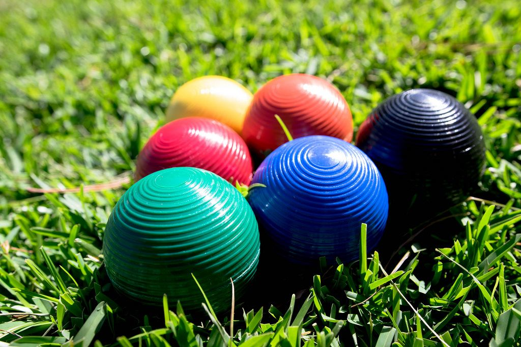
\includegraphics[width=80pt,height=60pt]{C6M04 - DT - Q1i.png}};
\draw (374.5,109.5) node  {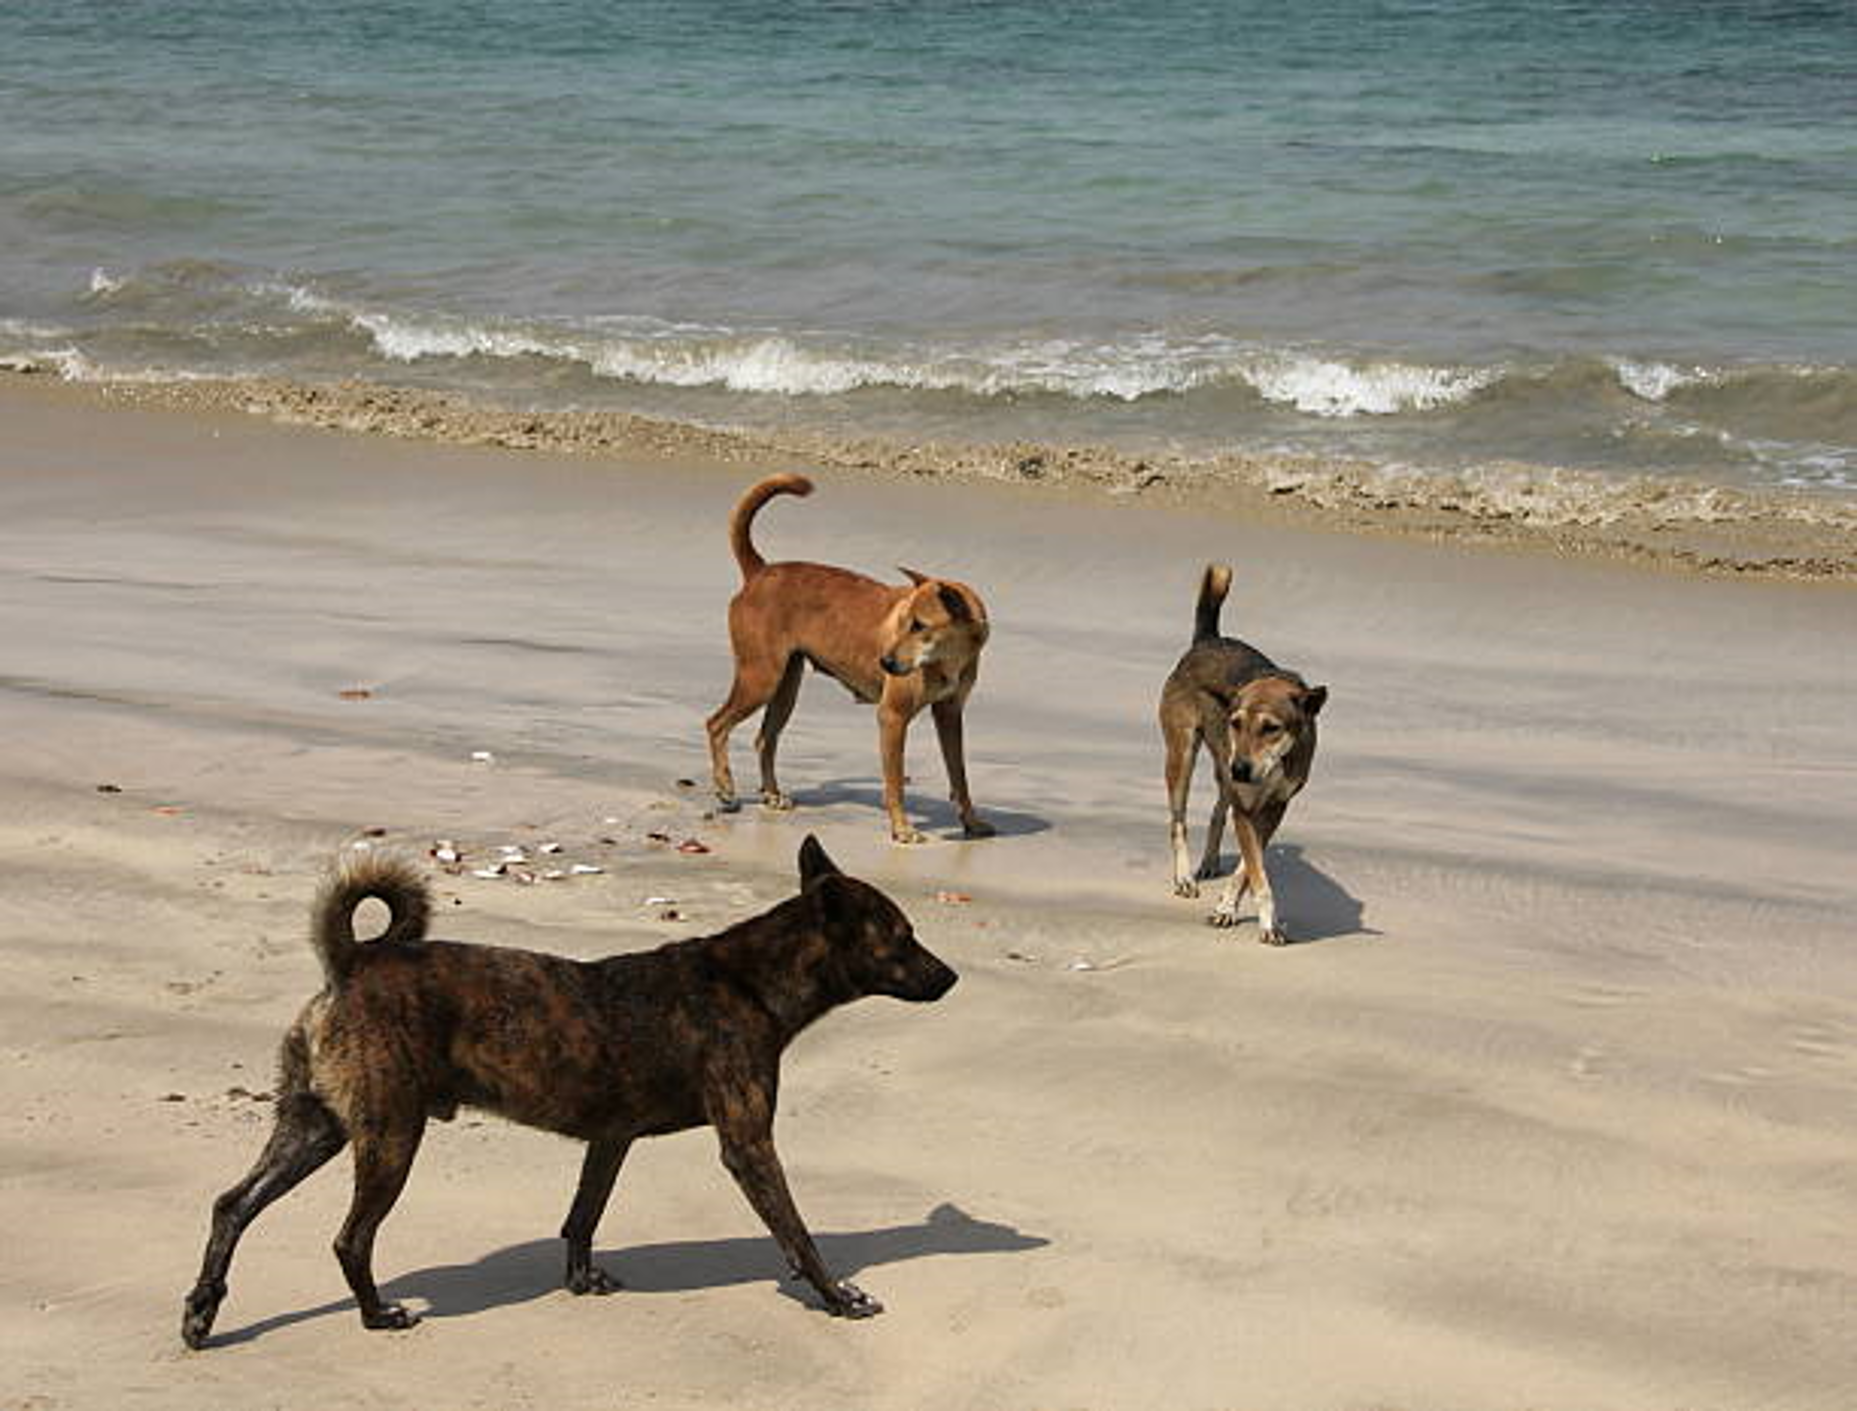
\includegraphics[width=80pt,height=60pt]{C6M04 - DT - Q1ii.png}};
\draw (90,155) node [anchor=north west][inner sep=0.75pt]   [align=left] {Number of balls = \rule{40pt}{0.5pt}};
\draw (295,155) node [anchor=north west][inner sep=0.75pt]   [align=left] {Number of dogs = \rule{40pt}{0.5pt}};
\end{tikzpicture}  
},
optionA={Balls},
optionB={Dogs},
optionC={Both balls and dogs},
optionD={None of these},
questionTag={C6M04 - DT - Q1}, 
leftmini={0.5},
rightmini={0.35},
correctoption={B},
}
% end-of-question

%-----------------------------------------------------------
%                        Question [ 26 ]
%-----------------------------------------------------------
% start-of-question
\mcqtextbottomOneFour{
questionnumber={2}, 
questiontext={Find all the factors of 8. },
optionA={1, 2, 8},
optionB={1, 2, 4, 8},
optionC={1, 2, 6},
optionD={4, 6, 8},
questionTag={C6M04 - DT - Q2}, 
correctoption={B},
}
% end-of-question

%-----------------------------------------------------------
%                        Question [ 27 ]
%-----------------------------------------------------------
% start-of-question
\mcqimgleftFourOne{
questionnumber={3}, 
questiontext={Daisy is asked to write the first five multiples of 9.},
imgtabletikz  = {  1 $\times$ 9 = \rule{40pt}{0.5pt}\\
2 $\times$ 9 = \rule{40pt}{0.5pt}\\
3 $\times$ 9 = \rule{40pt}{0.5pt}\\
4 $\times$ 9 = \rule{40pt}{0.5pt}\\ 
5 $\times$ 9 = \rule{40pt}{0.5pt}},
optionA={9, 11, 12, 13, 14},
optionB={9, 18, 36, 45, 54},
optionC={9, 18, 27, 36, 45},
optionD={19, 29, 39, 49, 59},
questionTag={C6M04 – DT – Q3}, 
correctoption={C},
leftmini={0.5},
rightmini={0.5}
}
% end-of-question

%-----------------------------------------------------------
%                        Question [ 28 ]
%-----------------------------------------------------------
% start-of-question
\mcqimgleftFourOne{
questionnumber={4}, 
questiontext={Match the following.},
imgtabletikz  = {
\renewcommand{\arraystretch}{1.25}
\begin{tabular}{|p{0.5cm}|p{1.6cm}|p{0.2cm}|p{0.5cm}|p{5.3cm}|}
\hline 
\multicolumn{2}{|c|}{\textbf{Numbers}} & 
\multirow{4}[10]{*}{} &   
\multicolumn{2}{c|}{\textbf{Type of Numbers }} \\
\cline{1-2}\cline{4-5} i & 1 &   & a & Neither prime nor composite \\
\cline{1-2}\cline{4-5} ii & 10 &   & b & Composite numbers  \\
\cline{1-2}\cline{4-5} iii & 5 &   & c & Prime numbers \\
\hline
\end{tabular} },
optionA={i - c, ii - b, iii - a},
optionB={i - a, ii - c, iii - b},
optionC={i - a, ii - b, iii - c},
optionD={i - b, ii - a, iii - c},
questionTag={C6M04 – DT – Q4}, 
correctoption={C},
leftmini={0.5},
rightmini={0.35}
}
% end-of-question

%-----------------------------------------------------------
%                        Question [ 29 ]
%-----------------------------------------------------------
% start-of-question
\mcqtextbottomOneFour{
questionnumber={5}, 
questiontext={Find the unit digit of the number 7910.},
optionA={0},
optionB={4},
optionC={7},
optionD={1},
questionTag={C6M04 - DT - Q5}, 
correctoption={A},
}
% end-of-question

%-----------------------------------------------------------
%                        Question [ 30 ]
%-----------------------------------------------------------
% start-of-question
\mcqimgleftFourOne{
questionnumber={6}, 
questiontext={The given amount is divisible by \rule{40pt}{0.5pt}.},
imgtabletikz = { 
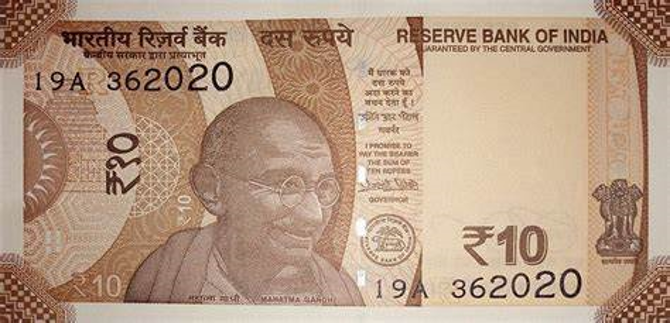
\includegraphics[width=6cm, height=2.5cm]{C6M04 - DT - Q6.png} },
optionA={5},
optionB={3},
optionC={4},
optionD={6},
questionTag={C6M04 - DT - Q6}, 
leftmini={0.4},
rightmini={0.4},
correctoption={A},
}
% end-of-question

%-----------------------------------------------------------
%                        Question [ 31 ]
%-----------------------------------------------------------
% start-of-question
\mcqtextbottomOneFour{
questionnumber={7}, 
questiontext={Find the prime factorisation of 18.},
optionA={ 2 $\times$ 6 $\times$ 1},
optionB={6 $\times$ 1 $\times$ 3},
optionC={2 $\times$ 3 $\times$ 3},
optionD={2 $\times$ 2 $\times$ 3},
questionTag={C6M04 - DT - Q7},
correctoption={C},
}
% end-of-question

%-----------------------------------------------------------
%                        Question [ 32 ]
%-----------------------------------------------------------
% start-of-question
\mcqimgleftFourOne{
questionnumber={8}, 
questiontext={Find the number in the circle by completing the given LCM. },
imgtabletikz  = { 
\renewcommand{\arraystretch}{1.25}
\begin{tabular}{p{1cm}|p{0.5cm}p{1cm}}
  \RaggedLeft{2} & 4, & 6 \\
  \cline{2-3}
  \RaggedLeft{2} & 2,& \rule{20pt}{0.5pt}\\
  \cline{2-3}
  \RaggedLeft{{\large{\textcircled{\rule{10pt}{0.5pt}}}}} & \rule{20pt}{0.5pt}, & 3 \\
  \cline{2-3}
  & 1,& 1 \\
  \cline{2-3}          
\end{tabular}
},
optionA={1},
optionB={2},
optionC={0},
optionD={3},
questionTag={C6M04 - DT - Q8}, 
leftmini={0.5},
rightmini={0.4},
correctoption={D},
}
% end-of-question

%-----------------------------------------------------------
%                        Question [ 33 ]
%-----------------------------------------------------------
% start-of-question
\mcqtextbottomOneFour{
questionnumber={9}, 
questiontext={Find the highest common factor of 9 and 18.\\
\quad The factors of 9 are 1, 3 and 9.\\
\quad The factors of 18 are 1, 2, 3, 6, 9 and 18. },
optionA={1, 3, 9},
optionB={1, 3},
optionC={18},
optionD={9},
questionTag={C6M04 - DT - Q9}, 
correctoption={D},
}
% end-of-question


%-----------------------------------------------------------
%                        Question [  ]
%-----------------------------------------------------------
% start-of-question
\mcqtextbottomOneFour{
questionnumber={10}, 
questiontext={Which of the following option contains all the factors of 9? },
optionA={1, 3, 6, 9},
optionB={9, 18,  27},
optionC={1, 3, 9},
optionD={3, 3},
questionTag={C6M04 - DT - Q10}, 
correctoption={C},
}
% end-of-question

%-----------------------------------------------------------
%                        Question [ 32 ]
%-----------------------------------------------------------
% start-of-question
\mcqimgleftFourOne{
questionnumber={11}, 
questiontext={Find the number in the circle by completing the given LCM.  },
imgtabletikz  = { 
\renewcommand{\arraystretch}{1.25}
\begin{tabular}{p{1cm}|p{0.5cm}p{1cm}}
  \RaggedLeft{2} & 6, & 8 \\
  \cline{2-3}
            \RaggedLeft{{\large{\textcircled{\rule{10pt}{0.5pt}}}}} & 3,& \rule{20pt}{0.5pt}\\
  \cline{2-3}
    \RaggedLeft{2} & 3, & \rule{20pt}{0.5pt} \\
  \cline{2-3}
  \RaggedLeft{3} & 3, & \rule{20pt}{0.5pt} \\
  \cline{2-3}          
\end{tabular}
},
optionA={1},
optionB={6},
optionC={3},
optionD={2},
questionTag={C6M04 - DT - Q11}, 
leftmini={0.5},
rightmini={0.4},
correctoption={D},
}
% end-of-question

%-----------------------------------------------------------
%                        Question [ 25 ]
%-----------------------------------------------------------
% start-of-question
\mcqimgleftFourOne{
questionnumber={12}, 
questiontext={Count the following dolls and identify their type.},
imgtabletikz  = {
\includegraphics[width=170pt,height=75pt]{C6M04 - DT - Q12.png} },
optionA={Odd number},
optionB={Even number},
optionC={Zero},
optionD={Cannot be determined},
questionTag={C6M04 - DT - Q12}, 
leftmini={0.5},
rightmini={0.35},
correctoption={A},
}
% end-of-question

%-----------------------------------------------------------
%                        Question [ 30 ]
%-----------------------------------------------------------
% start-of-question
\mcqtextbottomOneFour{
questionnumber={13}, 
questiontext={18 is divisible by \rule{40pt}{0.5pt}.},
optionA={2},
optionB={3},
optionC={6},
optionD={All the above},
questionTag={C6M04 - DT - Q13}, 
correctoption={D},
}
% end-of-question

%-----------------------------------------------------------
%                        Question [ 31 ]
%-----------------------------------------------------------
% start-of-question
\mcqimgleftFourOne{
questionnumber={14}, 
questiontext={Find the prime factors of 25.},
imgtabletikz  = { 
\renewcommand{\arraystretch}{1.3}
\begin{tabular}{p{1cm}|p{2cm}}
  \RaggedLeft{5} & 25 \\
  \cline{2-2}
  & \\
  \cline{2-2}
  & 1 \\
  \cline{2-2}          
\end{tabular}
},
optionA={ 5 $\times$ 5 $\times$ 1},
optionB={5 $\times$ 1 },
optionC={2 $\times$ 5 },
optionD={25 $\times$ 1},
questionTag={C6M04 - DT - Q14},
leftmini={0.5},
rightmini={0.4},
correctoption={A},
}
% end-of-question

%-----------------------------------------------------------
%                        Question [ 34 ]
%-----------------------------------------------------------
% start-of-question
\mcqtextbottomOneFour{
questionnumber={1}, 
questiontext={Count the number of points.\\
\medskip
\tikzset{every picture/.style={line width=0.75pt}} 
\hspace{2cm}
\begin{tikzpicture}[x=0.75pt,y=0.75pt,yscale=-1,xscale=1]
\draw    (102,111.97) -- (405,107.03) ;
\draw [shift={(407,107)}, rotate = 179.07] [color={rgb, 255:red, 0; green, 0; blue, 0 }  ][line width=0.75]    (10.93,-4.9) .. controls (6.95,-2.3) and (3.31,-0.67) .. (0,0) .. controls (3.31,0.67) and (6.95,2.3) .. (10.93,4.9)   ;
\draw [shift={(100,112)}, rotate = 359.07] [color={rgb, 255:red, 0; green, 0; blue, 0 }  ][line width=0.75]    (10.93,-4.9) .. controls (6.95,-2.3) and (3.31,-0.67) .. (0,0) .. controls (3.31,0.67) and (6.95,2.3) .. (10.93,4.9)   ;
\draw  [fill={rgb, 255:red, 74; green, 74; blue, 74 }  ,fill opacity=1 ] (147,112.5) .. controls (147,110.57) and (148.57,109) .. (150.5,109) .. controls (152.43,109) and (154,110.57) .. (154,112.5) .. controls (154,114.43) and (152.43,116) .. (150.5,116) .. controls (148.57,116) and (147,114.43) .. (147,112.5) -- cycle ;
\draw  [fill={rgb, 255:red, 74; green, 74; blue, 74 }  ,fill opacity=1 ] (196,110.5) .. controls (196,108.57) and (197.57,107) .. (199.5,107) .. controls (201.43,107) and (203,108.57) .. (203,110.5) .. controls (203,112.43) and (201.43,114) .. (199.5,114) .. controls (197.57,114) and (196,112.43) .. (196,110.5) -- cycle ;
\draw  [fill={rgb, 255:red, 74; green, 74; blue, 74 }  ,fill opacity=1 ] (255,109.5) .. controls (255,107.57) and (256.57,106) .. (258.5,106) .. controls (260.43,106) and (262,107.57) .. (262,109.5) .. controls (262,111.43) and (260.43,113) .. (258.5,113) .. controls (256.57,113) and (255,111.43) .. (255,109.5) -- cycle ;
\draw  [fill={rgb, 255:red, 74; green, 74; blue, 74 }  ,fill opacity=1 ] (293,109.5) .. controls (293,107.57) and (294.57,106) .. (296.5,106) .. controls (298.43,106) and (300,107.57) .. (300,109.5) .. controls (300,111.43) and (298.43,113) .. (296.5,113) .. controls (294.57,113) and (293,111.43) .. (293,109.5) -- cycle ;
\draw  [fill={rgb, 255:red, 74; green, 74; blue, 74 }  ,fill opacity=1 ] (347,108.5) .. controls (347,106.57) and (348.57,105) .. (350.5,105) .. controls (352.43,105) and (354,106.57) .. (354,108.5) .. controls (354,110.43) and (352.43,112) .. (350.5,112) .. controls (348.57,112) and (347,110.43) .. (347,108.5) -- cycle ;
\end{tikzpicture}
},
optionA={Four},
optionB={Five},
optionC={One},
optionD={Zero},
questionTag={C6M11 – DT – Q1}, 
correctoption={B},
}
% end-of-question

%-----------------------------------------------------------
%                        Question [ 35 ]
%-----------------------------------------------------------
% start-of-question
\mcqimgleftFourOne{
questionnumber={2}, 
questiontext={Match the following.},
imgtabletikz  = { 
\renewcommand{\arraystretch}{1.25}
\begin{tabular}{|p{0.5cm}|p{2.5cm}|p{0.3cm}|p{0.5cm}|p{3.5cm}|}
\hline
\multicolumn{2}{|c|}{\textbf{Symbols}} & 
\multirow{4}[10]{*}{} &   
\multicolumn{2}{c|}{\textbf{Names}} \\
\cline{1-2}\cline{4-5} i & 
\tikzset{every picture/.style={line width=0.75pt}} 
\begin{tikzpicture}[x=0.75pt,y=0.75pt,yscale=-1,xscale=1]
\draw    (100,120) -- (172,120) ;
\draw [shift={(174,120)}, rotate = 180] [color={rgb, 255:red, 0; green, 0; blue, 0 }  ][line width=0.75]    (10.93,-4.9) .. controls (6.95,-2.3) and (3.31,-0.67) .. (0,0) .. controls (3.31,0.67) and (6.95,2.3) .. (10.93,4.9)   ;
\draw [shift={(100,120)}, rotate = 0] [color={rgb, 255:red, 0; green, 0; blue, 0 }  ][fill={rgb, 255:red, 0; green, 0; blue, 0 }  ][line width=0.75]      (0, 0) circle [x radius= 3.35, y radius= 3.35]   ;
\end{tikzpicture}
&   & a & Line segment\\
\cline{1-2}\cline{4-5} ii &  

\tikzset{every picture/.style={line width=0.75pt}} 
\begin{tikzpicture}[x=0.75pt,y=0.75pt,yscale=-1,xscale=1]
\draw    (102,120) -- (172,120) ;
\draw [shift={(174,120)}, rotate = 180] [color={rgb, 255:red, 0; green, 0; blue, 0 }  ][line width=0.75]    (10.93,-4.9) .. controls (6.95,-2.3) and (3.31,-0.67) .. (0,0) .. controls (3.31,0.67) and (6.95,2.3) .. (10.93,4.9)   ;
\draw [shift={(100,120)}, rotate = 0] [color={rgb, 255:red, 0; green, 0; blue, 0 }  ][line width=0.75]    (10.93,-4.9) .. controls (6.95,-2.3) and (3.31,-0.67) .. (0,0) .. controls (3.31,0.67) and (6.95,2.3) .. (10.93,4.9)   ;
\end{tikzpicture}
&   & b & Ray\\
\cline{1-2}\cline{4-5} iii & 

\tikzset{every picture/.style={line width=0.75pt}} 
\begin{tikzpicture}[x=0.75pt,y=0.75pt,yscale=-1,xscale=1]
\draw    (100,120) -- (174,120) ;
\draw [shift={(174,120)}, rotate = 0] [color={rgb, 255:red, 0; green, 0; blue, 0 }  ][fill={rgb, 255:red, 0; green, 0; blue, 0 }  ][line width=0.75]      (0, 0) circle [x radius= 3.35, y radius= 3.35]   ;
\draw [shift={(100,120)}, rotate = 0] [color={rgb, 255:red, 0; green, 0; blue, 0 }  ][fill={rgb, 255:red, 0; green, 0; blue, 0 }  ][line width=0.75]      (0, 0) circle [x radius= 3.35, y radius= 3.35]   ;
\end{tikzpicture}
&   & c & Line \\
\hline
\end{tabular} },
optionA={i - b, ii - c, iii - a},
optionB={i - a, ii - b, iii - c},
optionC={i - c, ii - b, iii - a},
optionD={i - a, ii - c, iii - b},
questionTag={C6M11 – DT – Q2}, 
correctoption={A},
leftmini={0.5},
rightmini={0.35}
}
% end-of-question

%-----------------------------------------------------------
%                        Question [ 36 ]
%-----------------------------------------------------------
% start-of-question
\mcqimgleftFourOne{
questionnumber={3}, 
questiontext={The given lines are \rule{80pt}{0.5pt}.},
imgtabletikz = { 
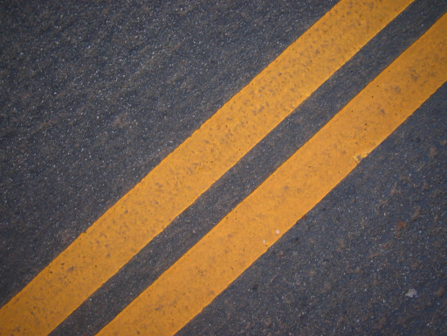
\includegraphics[width=2.5cm, height=2.5cm]{C6M11 - DT - Q3.png} },
optionA={Perpendicular lines},
optionB={Intersecting lines},
optionC={Parallel lines},
optionD={None of these},
questionTag={C6M11 - DT - Q3}, 
correctoption={C},
leftmini={0.3},
rightmini={0.6}
}
% end-of-question
%-----------------------------------------------------------
%                        Question [ 33 ]
%-----------------------------------------------------------
% start-of-question
\mcqtextbottomOneFour{
questionnumber={4}, 
questiontext={Which teddy bear shows an incorrect measurement of angles?},
optionA={ 
\includegraphics[height= 2cm, width=2.8cm]{C6M11 - DT - Q4i.png}  },
optionB={
\includegraphics[height= 2cm, width=2.8cm]{C6M11 - DT - Q4ii.png}  },
optionC={
\includegraphics[height= 2cm, width=2.8cm]{C6M11 - DT - Q4iii.png} },
optionD={ All the above},
questionTag={C6M11 - DT - Q4}, 
correctoption={D},
}
% end-of-question

%-----------------------------------------------------------
%                        Question [ 37 ]
%-----------------------------------------------------------
% start-of-question
\mcqimgleftFourOne{
questionnumber={5}, 
questiontext={The adjacent angles in the given figure are $\angle$XOY and \rule{50pt}{0.5pt}.},
imgtabletikz  = {
\tikzset{every picture/.style={line width=0.75pt}} 
\begin{tikzpicture}[x=0.75pt,y=0.75pt,yscale=-0.8,xscale=0.8]
\draw    (147,131) -- (263.4,44.2) ;
\draw [shift={(265,43)}, rotate = 143.29] [color={rgb, 255:red, 0; green, 0; blue, 0 }  ][line width=0.75]    (10.93,-4.9) .. controls (6.95,-2.3) and (3.31,-0.67) .. (0,0) .. controls (3.31,0.67) and (6.95,2.3) .. (10.93,4.9)   ;
\draw    (147,130) -- (290.04,99.42) ;
\draw [shift={(292,99)}, rotate = 167.93] [color={rgb, 255:red, 0; green, 0; blue, 0 }  ][line width=0.75]    (10.93,-4.9) .. controls (6.95,-2.3) and (3.31,-0.67) .. (0,0) .. controls (3.31,0.67) and (6.95,2.3) .. (10.93,4.9)   ; 
\draw    (147,131) -- (302,131) ;
\draw [shift={(304,131)}, rotate = 180] [color={rgb, 255:red, 0; green, 0; blue, 0 }  ][line width=0.75]    (10.93,-4.9) .. controls (6.95,-2.3) and (3.31,-0.67) .. (0,0) .. controls (3.31,0.67) and (6.95,2.3) .. (10.93,4.9)   ;
\draw (122,132) node [anchor=north west][inner sep=0.75pt]   [align=left] {O};
\draw (271,24) node [anchor=north west][inner sep=0.75pt]   [align=left] {X};
\draw (295,83) node [anchor=north west][inner sep=0.75pt]   [align=left] {Y};
\draw (309,125) node [anchor=north west][inner sep=0.75pt]   [align=left] {Z};
\end{tikzpicture}

},
optionA={$\angle$XOZ},
optionB={$\angle$YOX},
optionC={$\angle$YOZ},
optionD={$\angle$XYZ},
questionTag={C6M11 - DT - Q5}, 
correctoption={C},
leftmini={0.5},
rightmini={0.5}
}
% end-of-question

%-----------------------------------------------------------
%                        Question [ 38 ]
%-----------------------------------------------------------
% start-of-question
\mcqtextbottomOneFour{
questionnumber={6}, 
questiontext={Find the linear pair of angles.},
optionA={$180^\circ$, $180^\circ$},
optionB={$180^\circ$, $90^\circ$},
optionC={$90^\circ$ , $180^\circ$},
optionD={$90^\circ$, $90^\circ$},
questionTag={C6M11 - DT - Q6}, 
correctoption={D}
}
% end-of-question

%-----------------------------------------------------------
%                        Question [ 36 ]
%-----------------------------------------------------------
% start-of-question
\mcqtextbottomOneFour{
questionnumber={7}, 
questiontext={Find the figure with an open curve.},
optionA={
\tikzset{every picture/.style={line width=0.75pt}} 
\begin{tikzpicture}[x=0.75pt,y=0.75pt,yscale=-0.75,xscale=0.75] 
\draw   (100,121) -- (198,121) -- (180.06,134) -- (112,134) -- (112,183.31) -- (100,192) -- cycle ;
\end{tikzpicture} },
optionB={
\tikzset{every picture/.style={line width=0.75pt}} 
\begin{tikzpicture}[x=0.75pt,y=0.75pt,yscale=-0.75,xscale=0.75]
\draw   (270,45.5) .. controls (270,32.52) and (280.52,22) .. (293.5,22) .. controls (306.48,22) and (317,32.52) .. (317,45.5) .. controls (317,58.48) and (306.48,69) .. (293.5,69) .. controls (280.52,69) and (270,58.48) .. (270,45.5)(258,45.5) .. controls (258,25.89) and (273.89,10) .. (293.5,10) .. controls (313.11,10) and (329,25.89) .. (329,45.5) .. controls (329,65.11) and (313.11,81) .. (293.5,81) .. controls (273.89,81) and (258,65.11) .. (258,45.5) ;
\end{tikzpicture} },
optionC={
\tikzset{every picture/.style={line width=0.75pt}} 
\begin{tikzpicture}[x=0.75pt,y=0.75pt,yscale=-0.75,xscale=0.75]
\draw   (373.19,149.4) .. controls (376.26,155.12) and (378,161.61) .. (378,168.5) .. controls (378,191.42) and (358.75,210) .. (335,210) .. controls (311.25,210) and (292,191.42) .. (292,168.5) .. controls (292,145.58) and (311.25,127) .. (335,127) -- (335,168.5) -- cycle ;
\end{tikzpicture} },
optionD={
\tikzset{every picture/.style={line width=0.75pt}} 
\begin{tikzpicture}[x=0.75pt,y=0.75pt,yscale=-0.75,xscale=0.75] 
\draw  [draw opacity=0] (542.03,145.92) .. controls (547.81,141.58) and (555.09,139) .. (563,139) .. controls (581.78,139) and (597,153.55) .. (597,171.5) .. controls (597,189.45) and (581.78,204) .. (563,204) .. controls (546.07,204) and (532.03,192.17) .. (529.43,176.69) -- (563,171.5) -- cycle ; \draw   (542.03,145.92) .. controls (547.81,141.58) and (555.09,139) .. (563,139) .. controls (581.78,139) and (597,153.55) .. (597,171.5) .. controls (597,189.45) and (581.78,204) .. (563,204) .. controls (546.07,204) and (532.03,192.17) .. (529.43,176.69) ;  
\end{tikzpicture} },
questionTag={C6M11 – DT – Q7}, 
correctoption={D},
}
% end-of-question

%-----------------------------------------------------------
%                        Question [  ]
%-----------------------------------------------------------
% start-of-question
\mcqtextbottomOneFour{
questionnumber={8}, 
questiontext={Find the vertex of the given angle.

\tikzset{every picture/.style={line width=0.75pt}} %set default line width to 0.75pt        

\begin{tikzpicture}[x=0.75pt,y=0.75pt,yscale=-1,xscale=1]
%uncomment if require: \path (0,300); %set diagram left start at 0, and has height of 300

%Straight Lines [id:da8454741102507886] 
\draw    (214,205) -- (366,205.51) ;
\draw [shift={(369,205.52)}, rotate = 180.19] [fill={rgb, 255:red, 0; green, 0; blue, 0 }  ][line width=0.08]  [draw opacity=0] (8.93,-4.29) -- (0,0) -- (8.93,4.29) -- cycle    ;
%Straight Lines [id:da4680146019731224] 
\draw    (267.81,80.28) -- (214,205) ;
\draw [shift={(269,77.52)}, rotate = 113.34] [fill={rgb, 255:red, 0; green, 0; blue, 0 }  ][line width=0.08]  [draw opacity=0] (8.93,-4.29) -- (0,0) -- (8.93,4.29) -- cycle    ;

% Text Node
\draw (255,58) node [anchor=north west][inner sep=0.75pt]   [align=left] {X};
% Text Node
\draw (371,208.52) node [anchor=north west][inner sep=0.75pt]   [align=left] {Z};
% Text Node
\draw (197,204) node [anchor=north west][inner sep=0.75pt]   [align=left] {Y};


\end{tikzpicture}
},
optionA={Y},
optionB={X},
optionC={Z},
optionD={O},
questionTag={C6M11 – DT – Q8}, 
correctoption={A},
}
% end-of-question

%-----------------------------------------------------------
%                        Question [  ]
%-----------------------------------------------------------
% start-of-question
\mcqtextbottomOneFour{
questionnumber={9}, 
questiontext={Protractor measures up to \rule{50pt}{0.5pt}.},
optionA={360$^\circ$},
optionB={90$^\circ$},
optionC={180$^\circ$},
optionD={0$^\circ$},
questionTag={C6M11 – DT – Q9}, 
correctoption={C},
}
% end-of-question

%-----------------------------------------------------------
%                        Question [  ]
%-----------------------------------------------------------
% start-of-question
\mcqtextbottomOneFour{
questionnumber={10}, 
questiontext={Name the angle that lies between 90$^\circ$ and 180$^\circ$.},
optionA={Right angle},
optionB={Straight angle},
optionC={Obtuse angle},
optionD={Reflex angle},
questionTag={C6M11 – DT – Q10}, 
correctoption={C},
}
% end-of-question

%-----------------------------------------------------------
%                        Question [ 39 ]
%-----------------------------------------------------------
% start-of-question
\mcqimgleftFourOne{
questionnumber={1}, 
questiontext={Name this polygon.},
imgtabletikz = { 
\tikzset{every picture/.style={line width=0.75pt}} 
\begin{tikzpicture}[x=0.75pt,y=0.75pt,yscale=-1,xscale=1]
\draw  [fill={rgb, 255:red, 245; green, 166; blue, 35 }  ,fill opacity=1 ] (235.87,155.27) -- (198.66,189.37) -- (148.23,187.17) -- (114.13,149.96) -- (116.33,99.53) -- (153.55,65.43) -- (203.97,67.63) -- (238.08,104.84) -- cycle ;
\draw  [fill={rgb, 255:red, 255; green, 255; blue, 255 }  ,fill opacity=1 ] (226.46,150.25) -- (195.58,178.54) -- (153.74,176.72) -- (125.44,145.84) -- (127.27,104) -- (158.15,75.7) -- (199.99,77.53) -- (228.28,108.41) -- cycle ;
\end{tikzpicture}},
optionA={Square},
optionB={Heptagon},
optionC={Octagon},
optionD={Pentagon},
questionTag={C6M12 - DT - Q1}, 
correctoption={C},
leftmini={0.45},
rightmini={0.45},
}
% end-of-question

%-----------------------------------------------------------
%                        Question [ 40 ]
%-----------------------------------------------------------

% start-of-question
\mcqtextbottomTwoTwo{
questionnumber={2}, 
questiontext={Find the odd one out. },
optionA={Scalene triangle - three unequal sides},
optionB={Isosceles triangle - two equal sides},
optionC={Equilateral triangle - three equal sides},
optionD={Right angled triangle – all sides equal },
questionTag={C6M12 - DT - Q2}, 
correctoption={D},
}
% end-of-question

%-----------------------------------------------------------
%                        Question [ 41 ]
%-----------------------------------------------------------
% start-of-question

\mcqimgsideFourOne{
questionnumber={3}, 
questiontext={Match the following.},
imgwidth={9cm},
imgheight={4cm},
img={C6M12 - DT - Q3.png},
optionA={i - c, ii - d, iii - a, iv - b},
optionB={i - c, ii - b, iii - a, iv - d},
optionC={i - c, ii - d, iii - b, iv - a},
optionD={i - b, ii - a, iii - c, iv - d},
questionTag={C6M12 – DT – Q3}, 
leftmini={0.4},
rightmini={0.5}, 
correctoption={C},
}
% end-of-question

%-----------------------------------------------------------
%                        Question [ 42 ]
%-----------------------------------------------------------
% start-of-question
\mcqimgleftFourOne{
questionnumber={4}, 
questiontext={What does the line in the given figure represent?},
imgtabletikz  = {\tikzset{every picture/.style={line width=0.75pt}}
\hspace{3cm}
\begin{tikzpicture}[x=0.75pt,y=0.75pt,yscale=-0.75,xscale=0.75]
\draw    (86.5,105) -- (199.5,105) ;
\draw [shift={(202.5,105)}, rotate = 180] [fill={rgb, 255:red, 0; green, 0; blue, 0 }  ][line width=0.08]  [draw opacity=0] (6.25,-3) -- (0,0) -- (6.25,3) -- cycle    ;
\draw [shift={(83.5,105)}, rotate = 0] [fill={rgb, 255:red, 0; green, 0; blue, 0 }  ][line width=0.08]  [draw opacity=0] (6.25,-3) -- (0,0) -- (6.25,3) -- cycle    ; 
\draw   (83.5,105) .. controls (83.5,72.14) and (110.14,45.5) .. (143,45.5) .. controls (175.86,45.5) and (202.5,72.14) .. (202.5,105) .. controls (202.5,137.86) and (175.86,164.5) .. (143,164.5) .. controls (110.14,164.5) and (83.5,137.86) .. (83.5,105) -- cycle ;
\draw (135,85) node [anchor=north west][inner sep=0.75pt]   [align=left] {?};
\end{tikzpicture}},
optionA={Radius},
optionB={Vertices},
optionC={Diameter},
optionD={Circumference},
questionTag={C6M12 - DT - Q4}, 
correctoption={C},
leftmini={0.3},
rightmini={0.5}
}
% end-of-question

%-----------------------------------------------------------
%                        Question [ 40 ]
%-----------------------------------------------------------

% start-of-question
\mcqtextbottomTwoTwo{
questionnumber={5}, 
questiontext={A triangle with two equal sides is called \rule{80pt}{0.5pt}},
optionA={Scalene triangle},
optionB={Isosceles triangle},
optionC={Equilateral triangle},
optionD={Complementary triangle},
questionTag={C6M12 - DT - Q5}, 
correctoption={B},
}
% end-of-question

%-----------------------------------------------------------
%                        Question [ 43 ]
%-----------------------------------------------------------

% start-of-question
\mcqtextbottomTwoTwo{
questionnumber={1}, 
questiontext={3D shapes have \rule{80pt}{0.5pt}.},
optionA={Only length},
optionB={Length and breadth},
optionC={Only height},
optionD={ Length, breadth and height},
questionTag={C6M13 – DT – Q1}, 
correctoption={D},
}
% end-of-question


%-----------------------------------------------------------
%                        Question [ 44 ]
%-----------------------------------------------------------
% start-of-question
\mcqimgleftFourOne{
questionnumber={2}, 
questiontext={Identify the colour of the vertices.},
imgtabletikz = { 
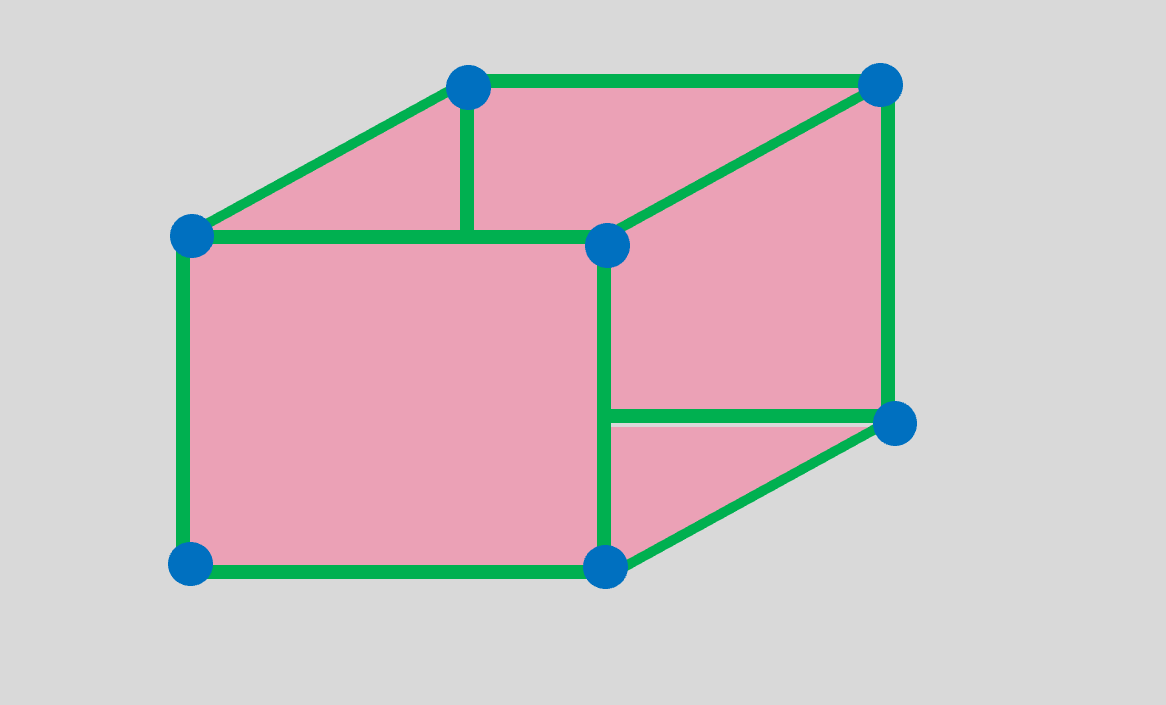
\includegraphics[width=5cm, height=3cm]{C6M13 - DT - Q2.png}},
optionA={Pink },
optionB={Blue},
optionC={Green },
optionD={Grey},
questionTag={C6M13 - DT - Q2}, 
correctoption={B},
leftmini={0.4},
rightmini={0.5}
}
% end-of-question

%-----------------------------------------------------------
%                        Question [ 45 ]
%-----------------------------------------------------------
% start-of-question
\mcqimgleftFourOne{
questionnumber={1}, 
questiontext={Represent the given number of ice creams in tallymarks.},
imgtabletikz = { 

\includegraphics[width=8cm, height=1.5cm]{C6M17 - DT - Q1.png}},
optionA={
\tikzset{every picture/.style={line width=0.75pt}}  
\begin{tikzpicture}[x=0.75pt,y=0.75pt,yscale=-1,xscale=1]
\draw    (120.33,68.14) -- (120.33,90.39) ;
\draw    (132.28,68) -- (132.28,90.25) ;
\draw    (143.36,68.28) -- (143.36,90.53) ;
\draw    (155.31,68.42) -- (155.31,90.67) ;
\draw    (143.36,68.28) -- (120.33,90.39) ;
\end{tikzpicture}
},
optionB={ 
\tikzset{every picture/.style={line width=0.75pt}} 
\begin{tikzpicture}[x=0.75pt,y=0.75pt,yscale=-1,xscale=1]
\draw    (100.31,116.42) -- (100.31,138.67) ;
\draw    (112.26,116) -- (112.26,138.25) ;
\draw    (123.33,116.14) -- (123.33,138.39) ;
\draw    (133.26,115.95) -- (133.26,138.19) ;
\draw    (144.33,116.09) -- (144.33,138.33) ;
\end{tikzpicture}
},
optionC={   
\tikzset{every picture/.style={line width=0.75pt}} 
\begin{tikzpicture}[x=0.75pt,y=0.75pt,yscale=-1,xscale=1]
\draw    (276.33,114.14) -- (276.33,136.39) ;
\draw    (288.28,114) -- (288.28,136.25) ;
\draw    (299.36,114.28) -- (299.36,136.53) ;
\draw    (311.31,114.42) -- (311.31,136.67) ;
\draw    (293.28,114) -- (270.28,136) ;
\draw    (323.26,114) -- (323.26,136.25) ;
\draw    (334.33,114.14) -- (334.33,136.39) ;
\draw    (344.26,113.95) -- (344.26,136.19) ;
\draw    (355.33,114.09) -- (355.33,136.33) ;
\draw    (316.28,116) -- (293.28,138) ;
\draw    (338.48,115) -- (315.48,137) ;
\draw    (360.33,114.39) -- (337.33,136.39) ;
\draw    (366.06,113.2) -- (366.06,135.45) ;
\draw    (377.13,113.34) -- (377.13,135.59) ;
\draw    (387.06,113.15) -- (387.06,135.39) ;
\draw    (398.13,113.29) -- (398.13,135.53) ;
\draw    (381.28,114.2) -- (358.28,136.2) ;
\draw    (403.13,113.59) -- (380.13,135.59) ;
\end{tikzpicture}
},
optionD={
\tikzset{every picture/.style={line width=0.75pt}} 
\begin{tikzpicture}[x=0.75pt,y=0.75pt,yscale=-1,xscale=1]
\draw    (98.33,161.14) -- (98.33,183.39) ;
\draw    (110.28,161) -- (110.28,183.25) ;
\draw    (121.36,161.28) -- (121.36,183.53) ;
\draw    (133.31,161.42) -- (133.31,183.67) ;
\draw    (133.31,161.42) -- (98.33,183.39) ;
\draw    (145.26,161) -- (145.26,183.25) ;
\end{tikzpicture}
},
questionTag={C6M17 – DT – Q1}, 
correctoption={D},
leftmini={0.5},
rightmini={0.4}
}
% end-of-question


%-----------------------------------------------------------
%                        Question [ 46 ]
%-----------------------------------------------------------
% start-of-question
\mcqimgleftFourOne{
questionnumber={2}, 
questiontext={Observe the given pictograph and find the number of roses sold on Thursday.},
imgtabletikz  = {
\renewcommand{\arraystretch}{1.25}
\begin{tabular}{|c|c|}
\hline
  Days & Number of roses sold (1 \smiley = 1 rose)  \\
  \hline
  Monday& \smiley \smiley \smiley  \\
  \hline
  Tuesday  & \smiley \smiley \smiley \smiley \smiley \smiley \smiley  \\
  \hline
  Wednesday & \smiley \smiley \smiley \smiley \smiley \smiley \smiley \smiley \\
  \hline
  Thursday & \smiley \smiley \smiley \smiley \smiley \smiley \\
  \hline
\end{tabular}  },
optionA={0},
optionB={8},
optionC={6},
optionD={7},
questionTag={C6M17 - DT - Q2}, 
leftmini={0.5},
rightmini={0.3},
correctoption={C},
}
% end-of-question

% %-----------------------------------------------------------
% %                        Question [ 47 ]
% %-----------------------------------------------------------
% % start-of-question
% \mcqimgleftFourOne{
% questionnumber={3}, 
% questionTag={C6M17 – DT – Q3}, 
% questiontext={Find the number of fruits sold on Saturday.},
% imgtabletikz = { \VerticalBar{
%     Scale=1,
%     Width={17},
%     Height=12,
%     Barwidth=17,
%     Textwidth=2.2,
%     Xlabel={Percentage(\%)},
%     Xtick={1,2,3,4,5},
%     Xticklabels={{0\% to 20\%},{21\% to 40\%},{41\% to 60\%},{61\% to 80\%},{81\% to 100\%}},
%     Xlabelrotate=45,
%     Ylabels={Values},
%     Ytick={0,5,10,15,20},   
%     Barcoords={{2},{5},{3,2,5,3,2},{0,3,7,15,5}},
%     YMin=0,
%     YMax=20,
%     Title={Class 6 Math}
% }{Class 6A,Class 6B}%legend
% {7}%average
% },
% optionA={100},
% optionB={80},
% optionC={10},
% optionD={101},
% leftmini={0.65},
% rightmini={0.25},
% correctoption={A},
% }
% % end-of-question

%-----------------------------------------------------------
%                        Question [  ]
%-----------------------------------------------------------

% start-of-question
\mcqimgleftFourOne{
questionnumber={3}, 
questionTag={C6M17 – DT – Q3}, 
questiontext={Find the number of fruits sold on Saturday.},
imgtabletikz = { 
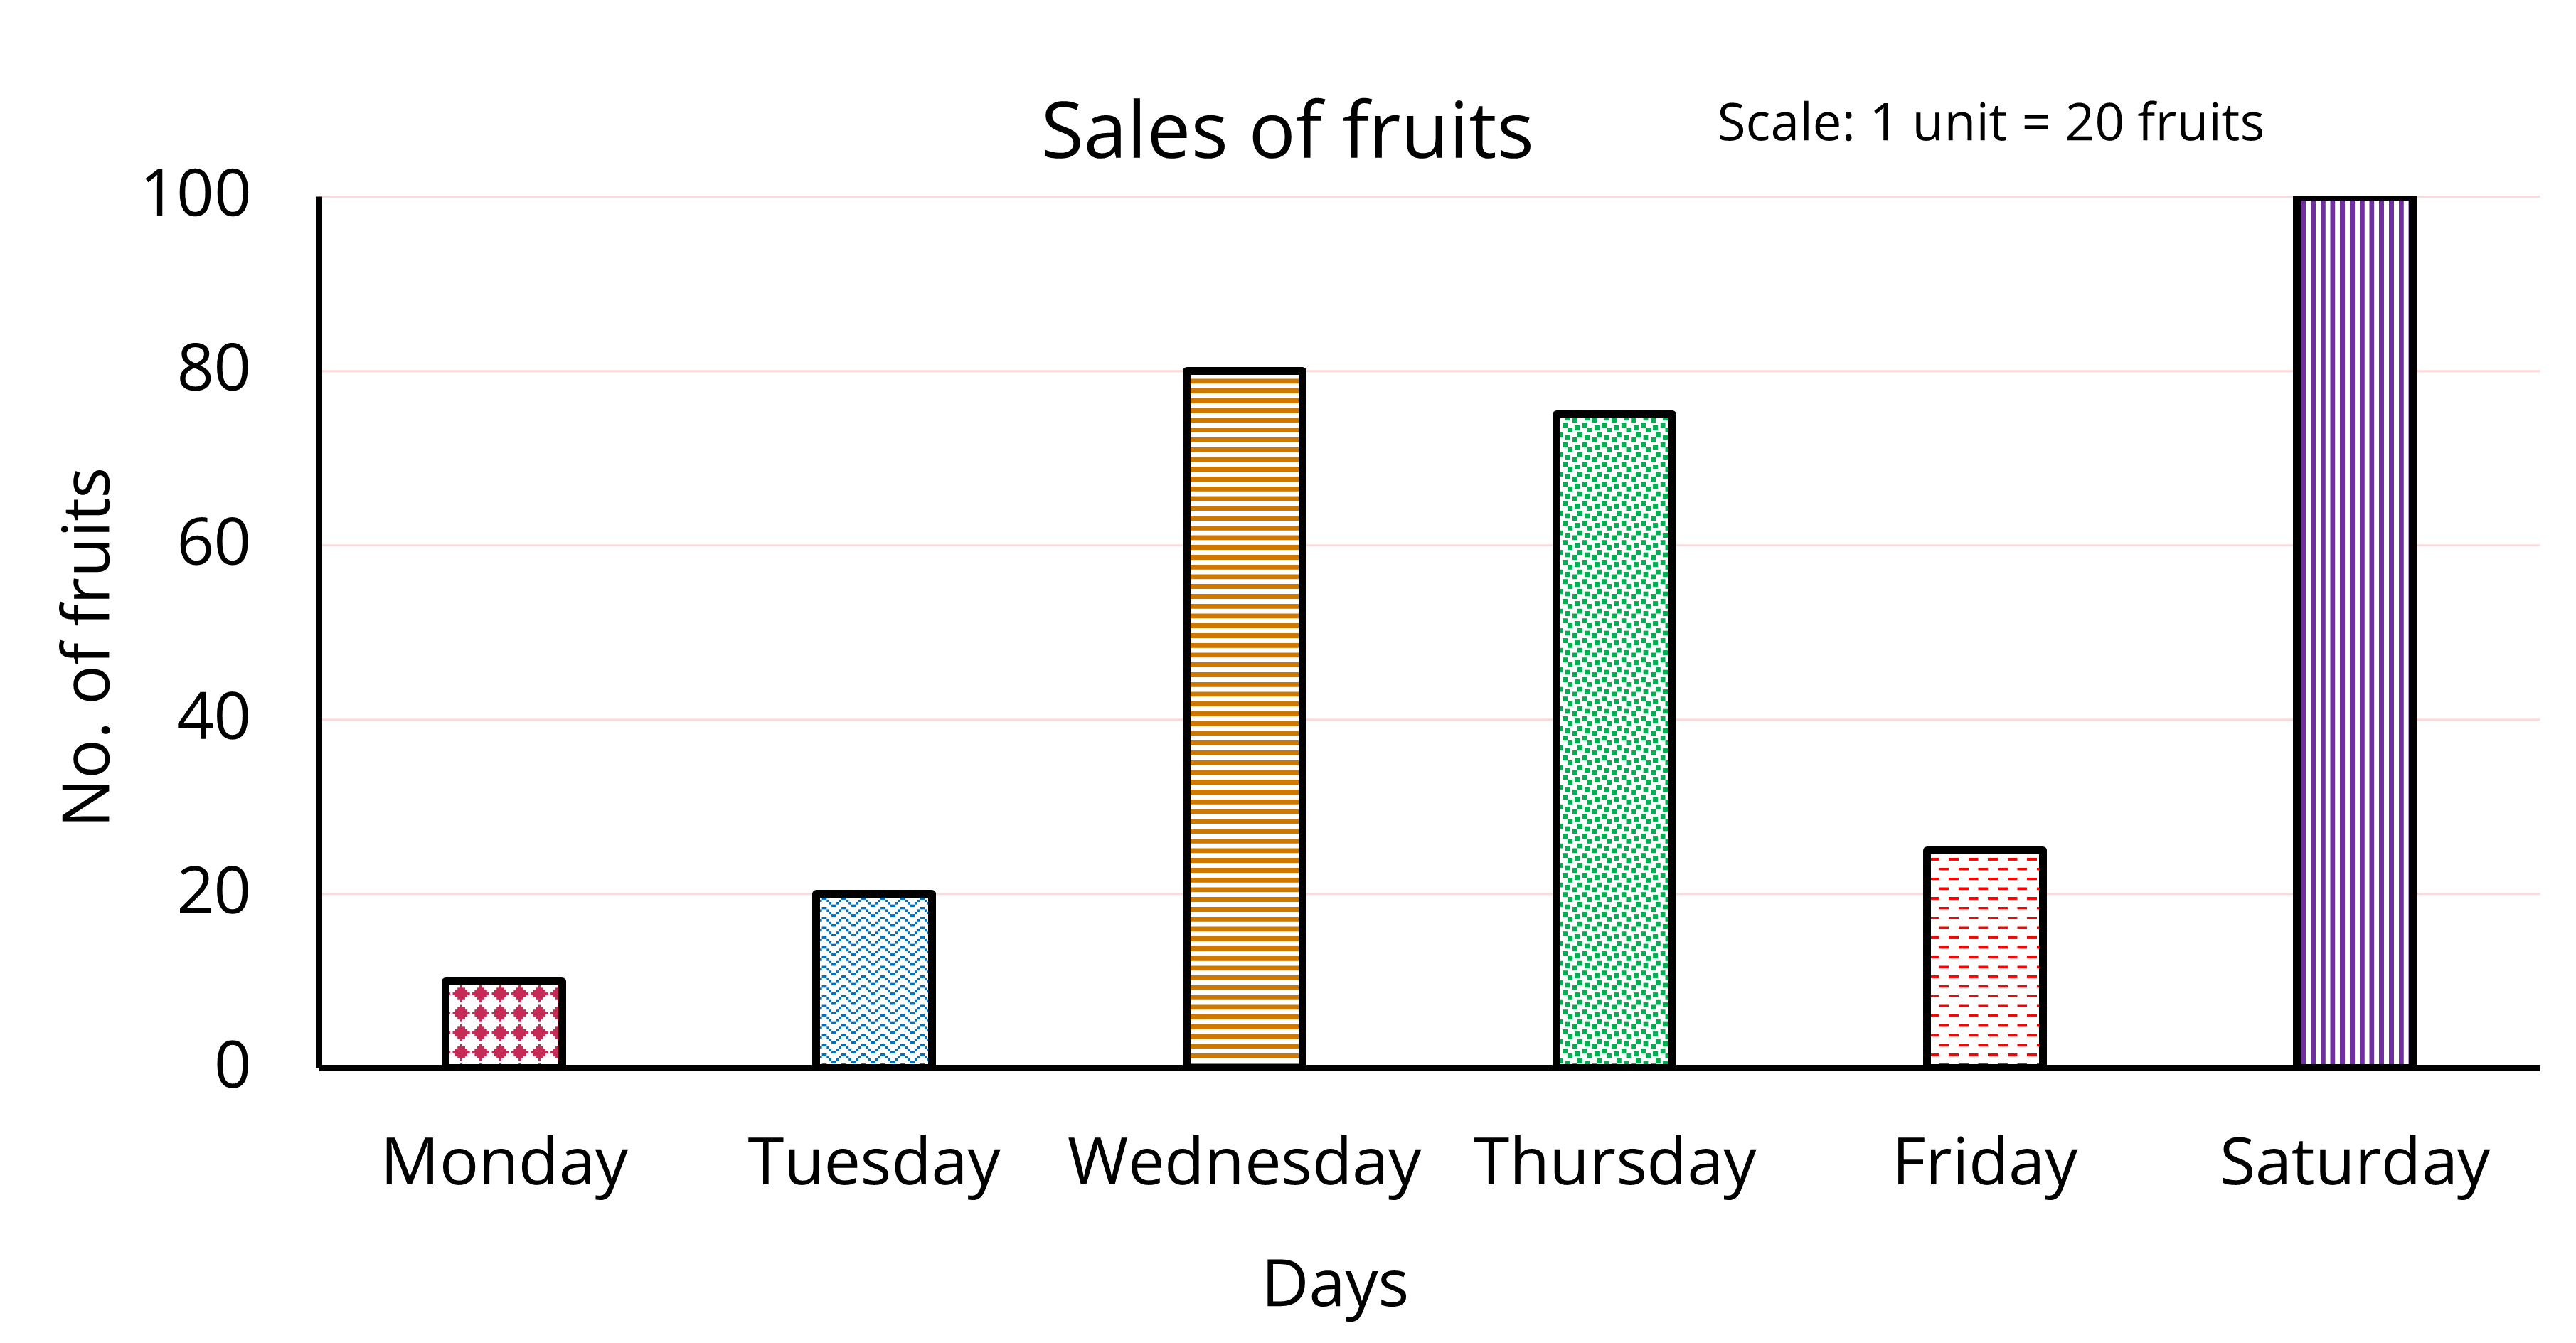
\includegraphics[width=12cm, height=6cm]{C6M17 - DT - Q3.png}},
optionA={100},
optionB={80},
optionC={10},
optionD={101},
leftmini={0.65},
rightmini={0.25},
correctoption={A},
}
% end-of-question

%-----------------------------------------------------------
%                        Question [  ]
%-----------------------------------------------------------
% start-of-question
\mcqtextbottomOneFour{
questionnumber={4}, 
questionTag={C6M17 - DT - Q4}, 
questiontext={
The school cafeteria manager is interested in understanding the lunch preferences of students. The representation below shows the number of students who prefer different lunch timings in ‘p.m.’ \\
\qquad 
1 p.m. 2 p.m. 3 p.m. 12 p.m. 1 p.m. 3 p.m. 2 p.m. 2 p.m. 1 p.m. 12 p.m. \\
Use tally marks to find the number of students who prefer to have lunch at 1 p.m. },
optionA={\begin{tikzpicture}[x=0.75pt,y=0.75pt,yscale=-1,xscale=1]
\draw    (20.33,9.14) -- (20.33,31.39) ;
\draw    (32.28,9) -- (32.28,31.25) ;
\draw    (43.36,9.28) -- (43.36,31.53) ;
\draw    (55.31,9.42) -- (55.31,31.67) ;
\draw    (55.31,9.42) -- (20.33,31.39) ;
\end{tikzpicture} },
optionB={
\begin{tikzpicture}[x=0.75pt,y=0.75pt,yscale=-1,xscale=1]
\draw    (20.33,9.14) -- (20.33,31.39) ;
\draw    (32.28,9) -- (32.28,31.25) ;
\draw    (43.36,9.28) -- (43.36,31.53) ;
\end{tikzpicture} 
},
optionC={
\begin{tikzpicture}[x=0.75pt,y=0.75pt,yscale=-1,xscale=1]
\draw    (20.33,9.14) -- (20.33,31.39) ;
\draw    (32.28,9) -- (32.28,31.25) ;
\draw    (43.36,9.28) -- (43.36,31.53) ;
\draw    (55.31,9.42) -- (55.31,31.67) ;
\end{tikzpicture} 
},
optionD={
\begin{tikzpicture}[x=0.75pt,y=0.75pt,yscale=-1,xscale=1]
\draw    (20.33,9.14) -- (20.33,31.39) ;
\draw    (32.28,9) -- (32.28,31.25) ;
\end{tikzpicture} 
},
correctoption={B},
}
% end-of-question

%-----------------------------------------------------------
%                        Question [  ]
%-----------------------------------------------------------
% start-of-question
\mcqimgleftFourOne{
questionnumber={5}, 
questiontext={Observe the pictograph and complete them.},
questionTag={C6M17 – DT – Q5},
imgtabletikz = { 
\begin{table}[H]
\centering
\renewcommand{\arraystretch}{2.5}
\begin{tabular}{|p{4.5cm}|p{3cm}|}
\hline
Number of students & Number of balls\\
\hline
5 students & 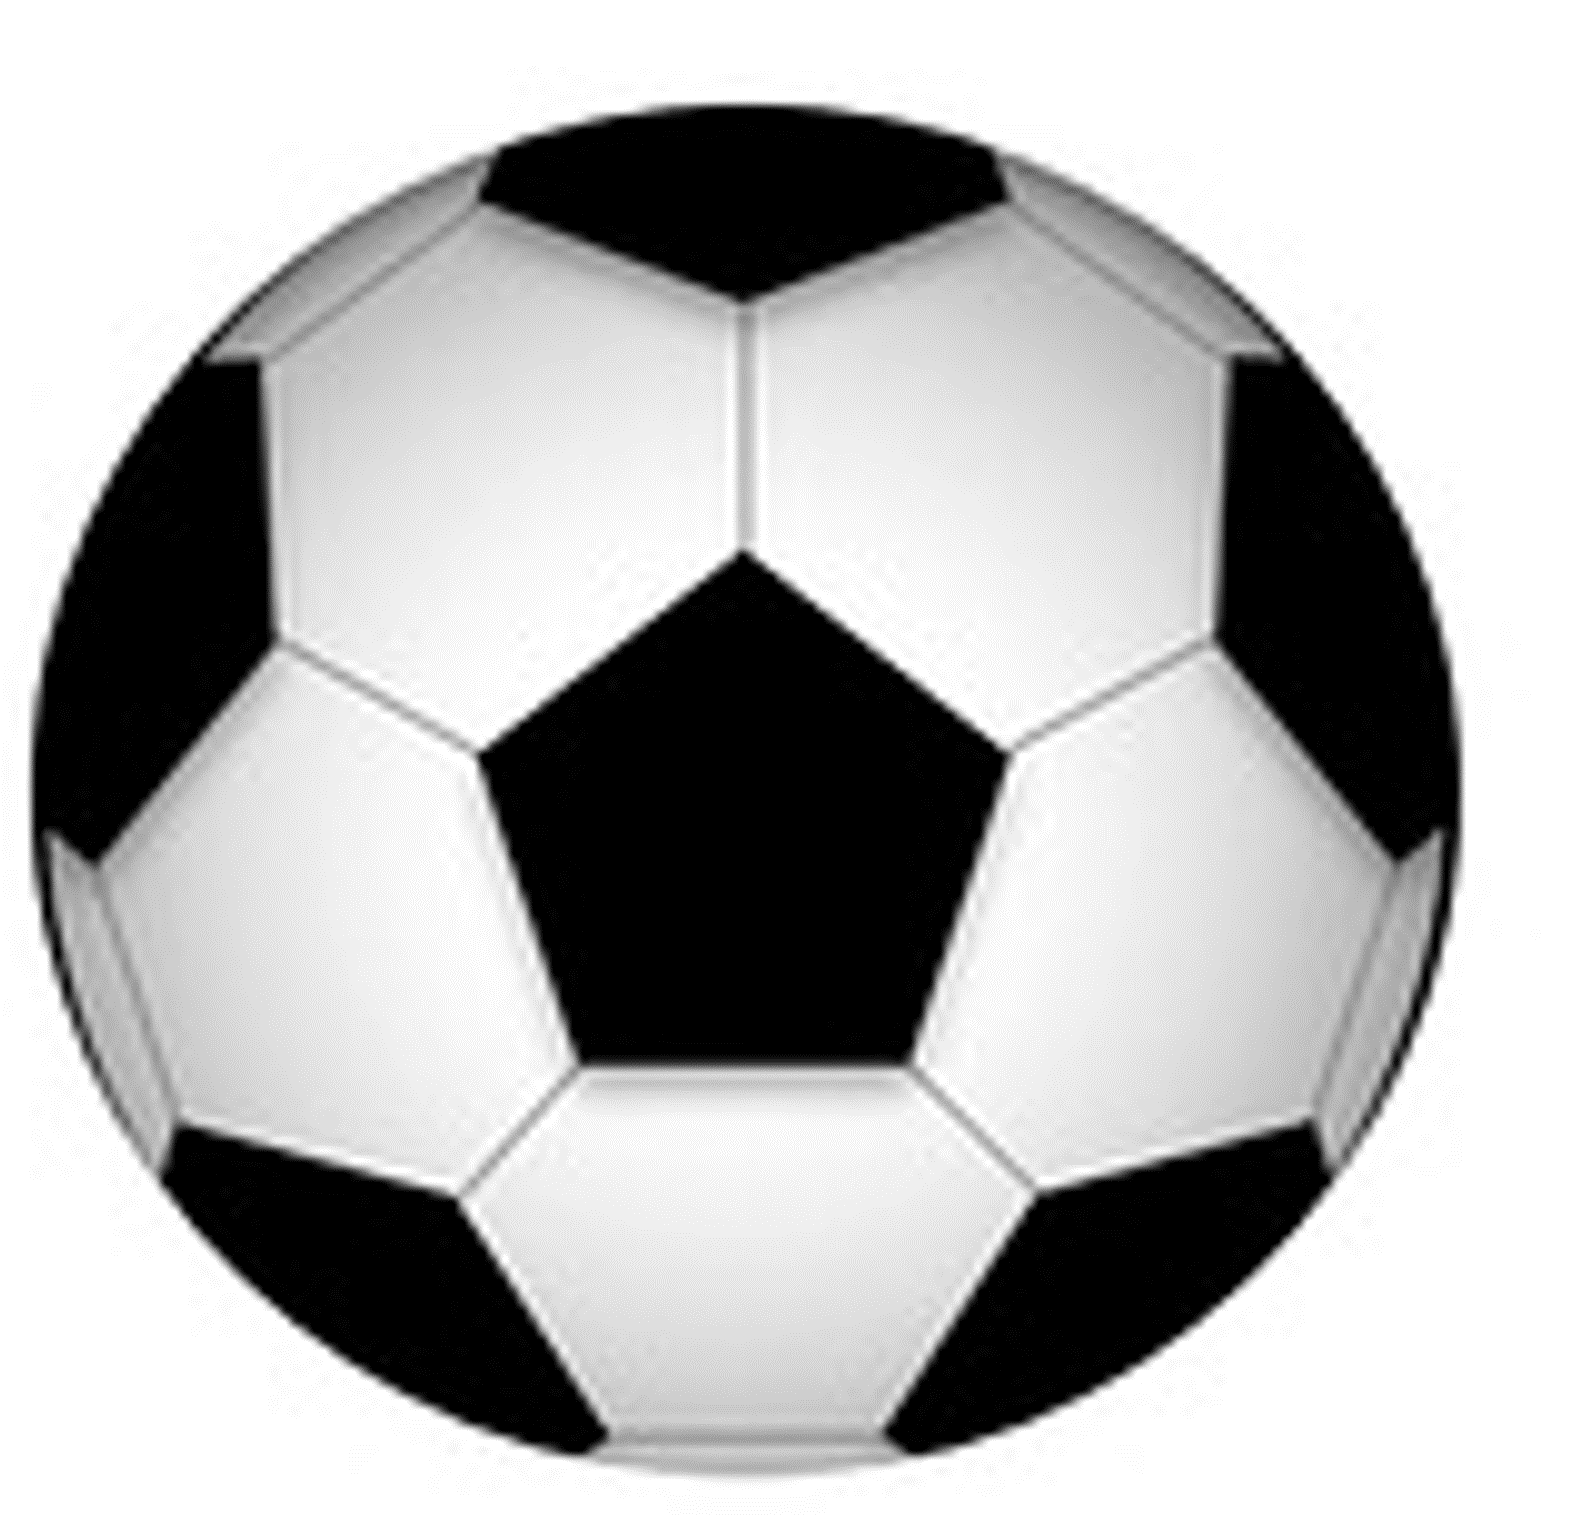
\includegraphics[width=1cm, height=1cm]{C6M17 - DT - Q5.png}\\
\hline
25 students & ? \\
\hline        
\end{tabular}
\end{table}
},
optionA={
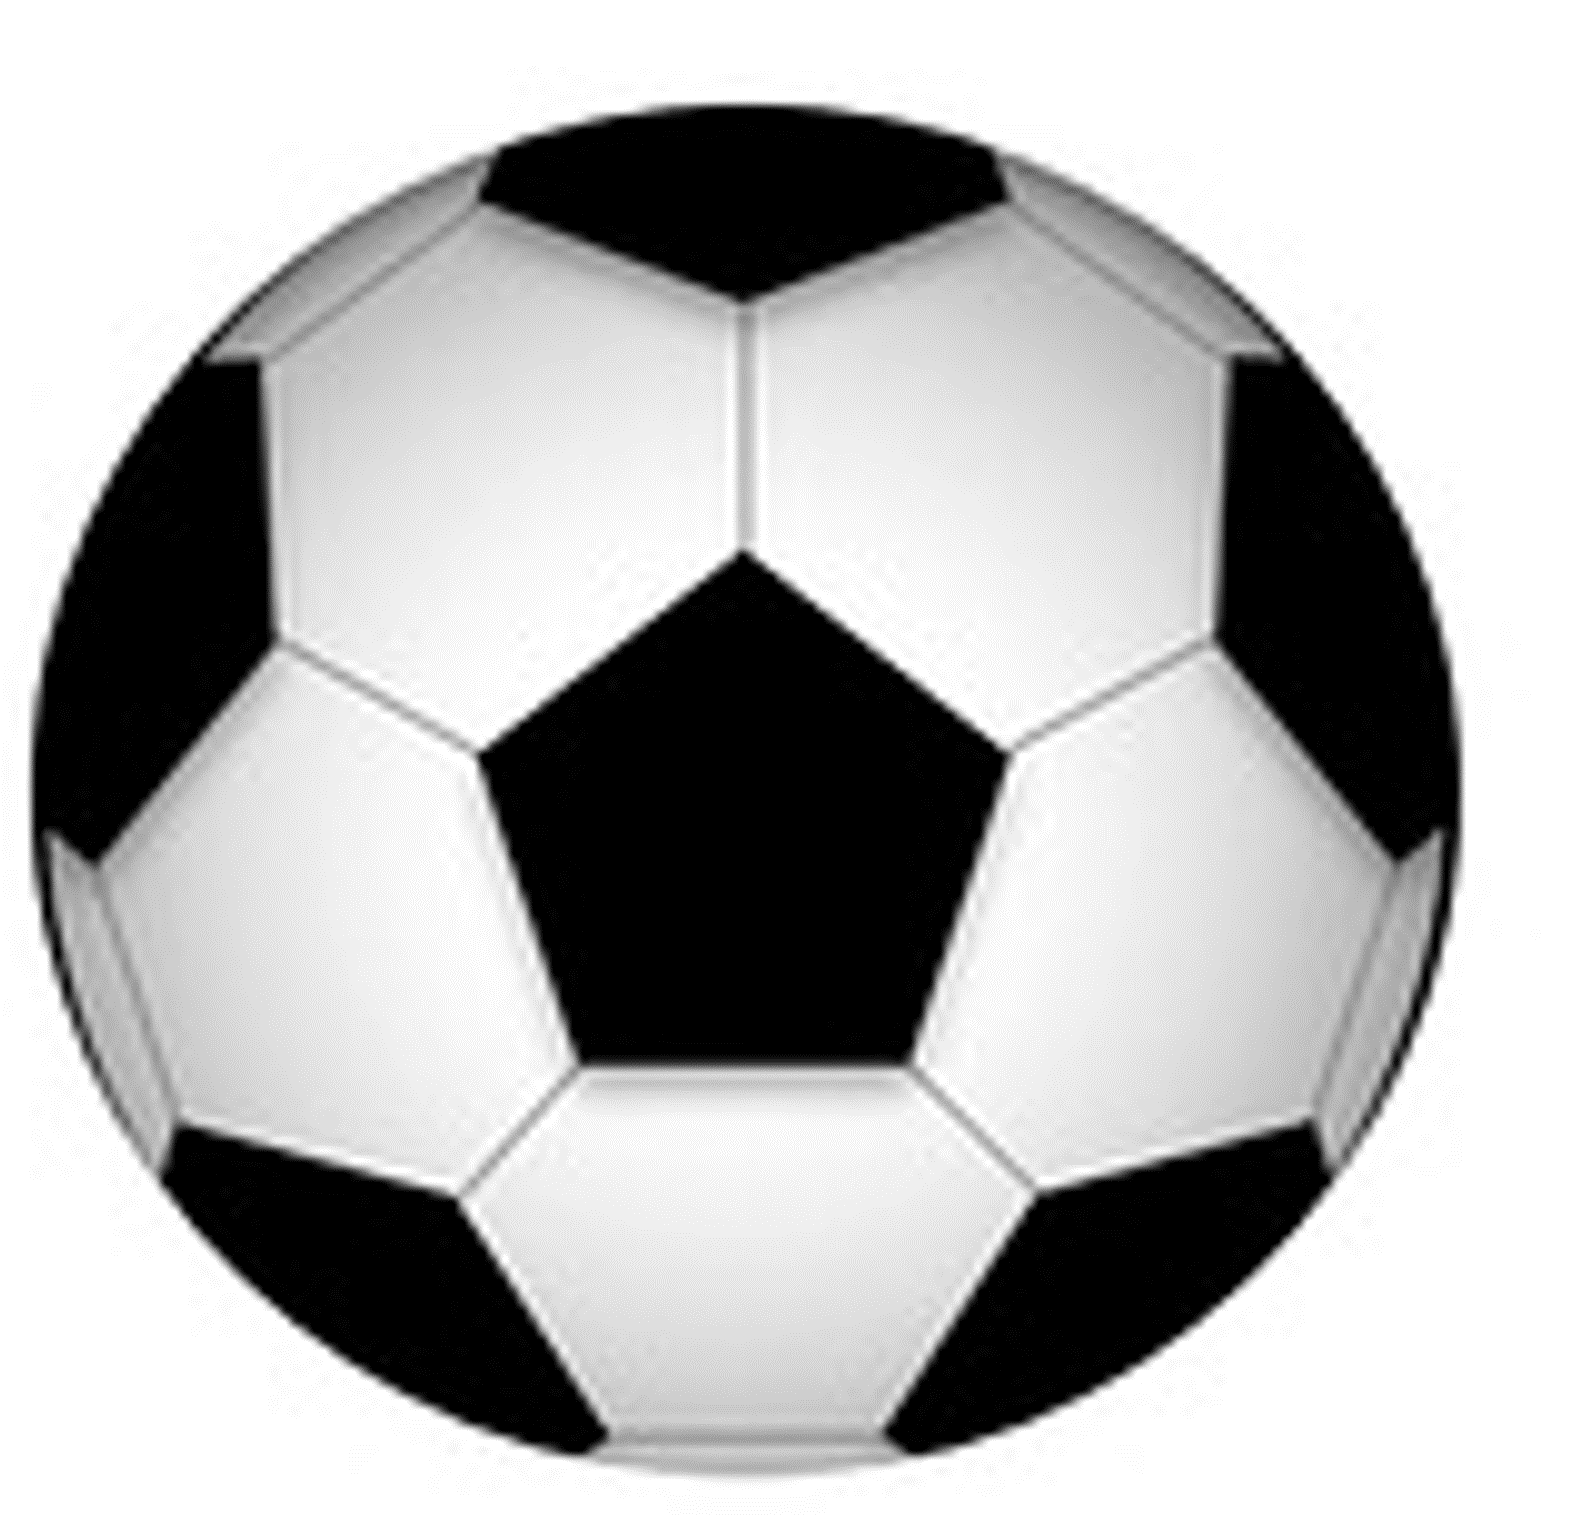
\includegraphics[width=1cm, height=1cm]{C6M17 - DT - Q5.png} 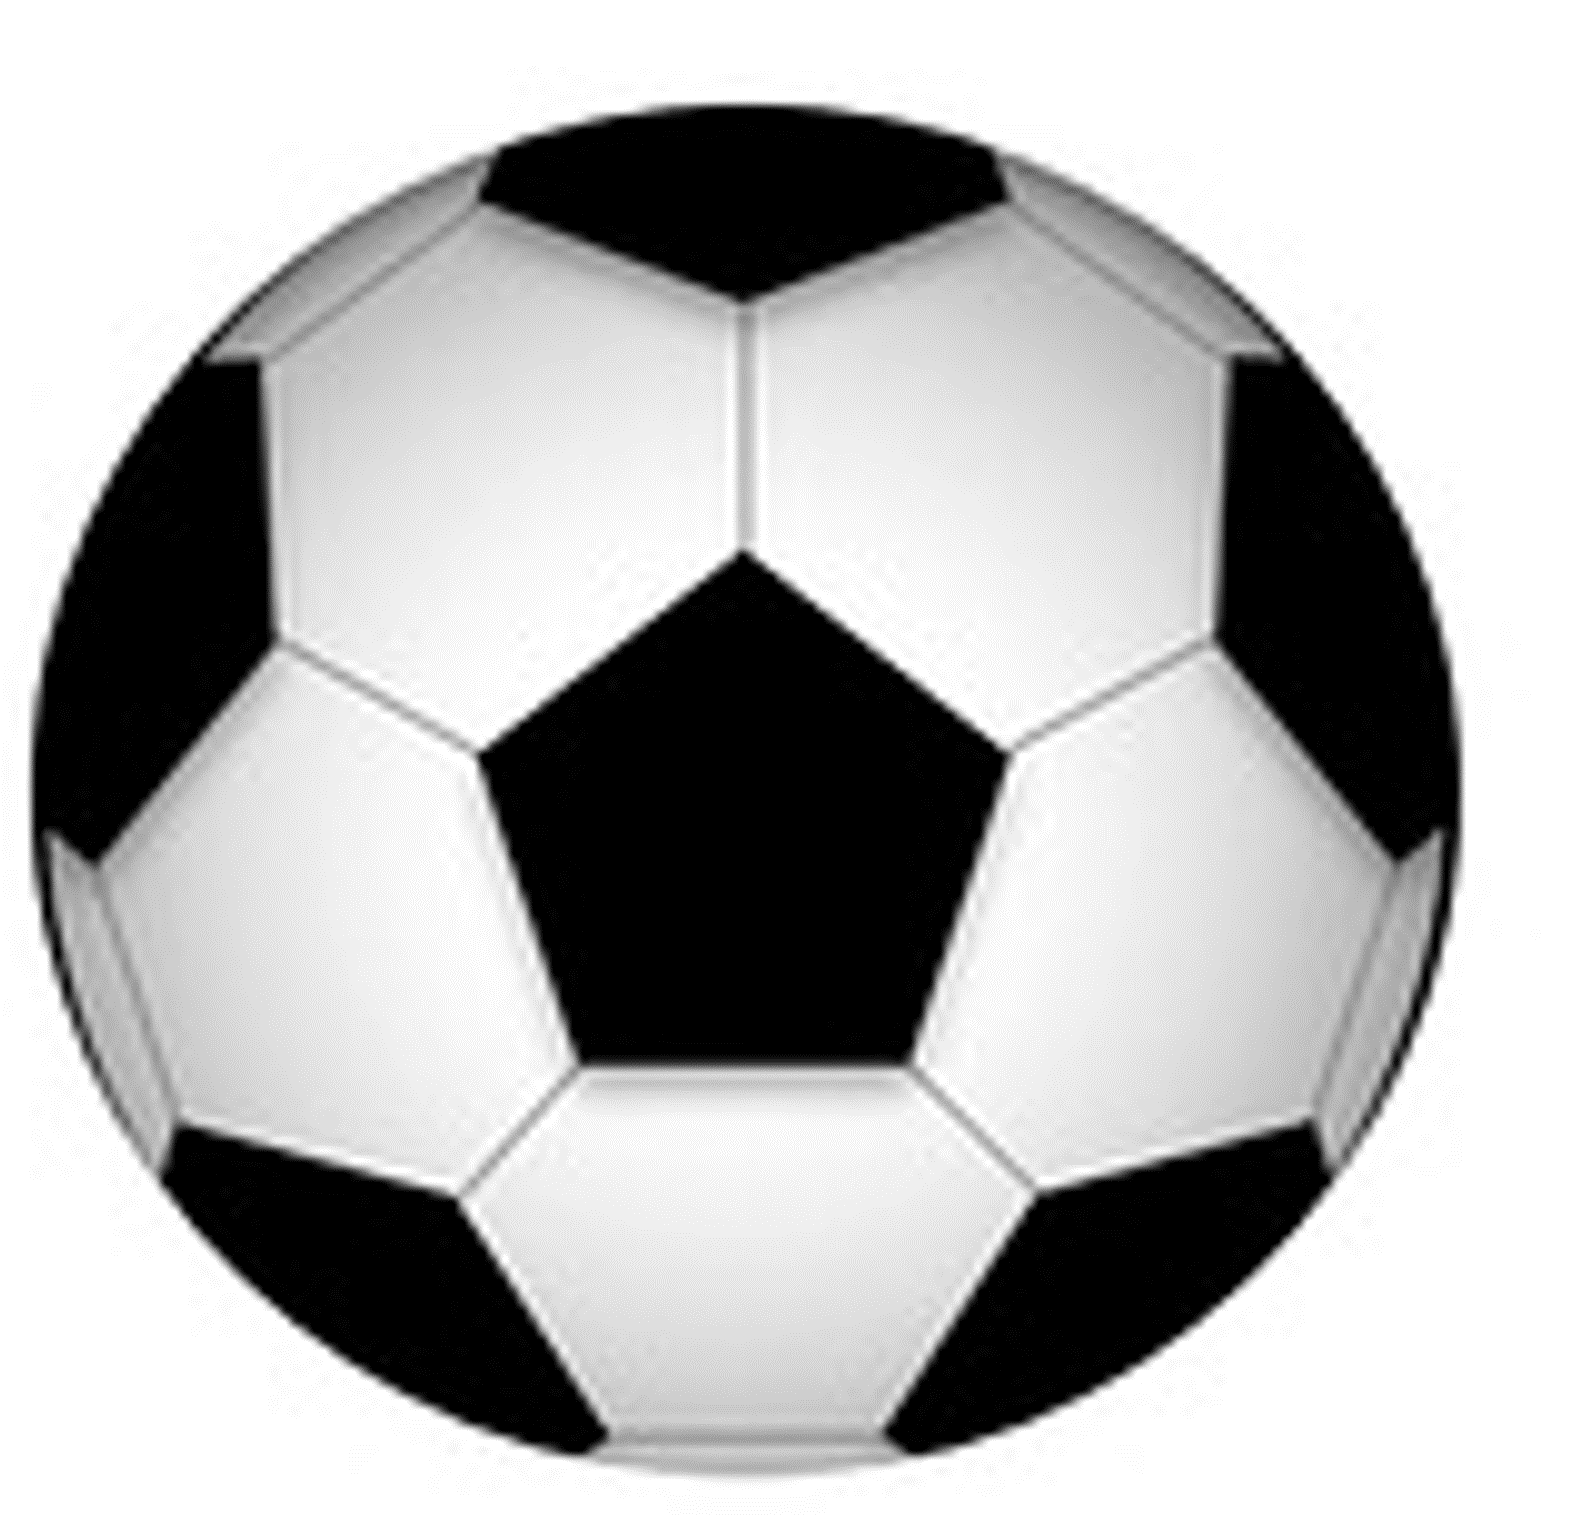
\includegraphics[width=1cm, height=1cm]{C6M17 - DT - Q5.png} },
optionB={
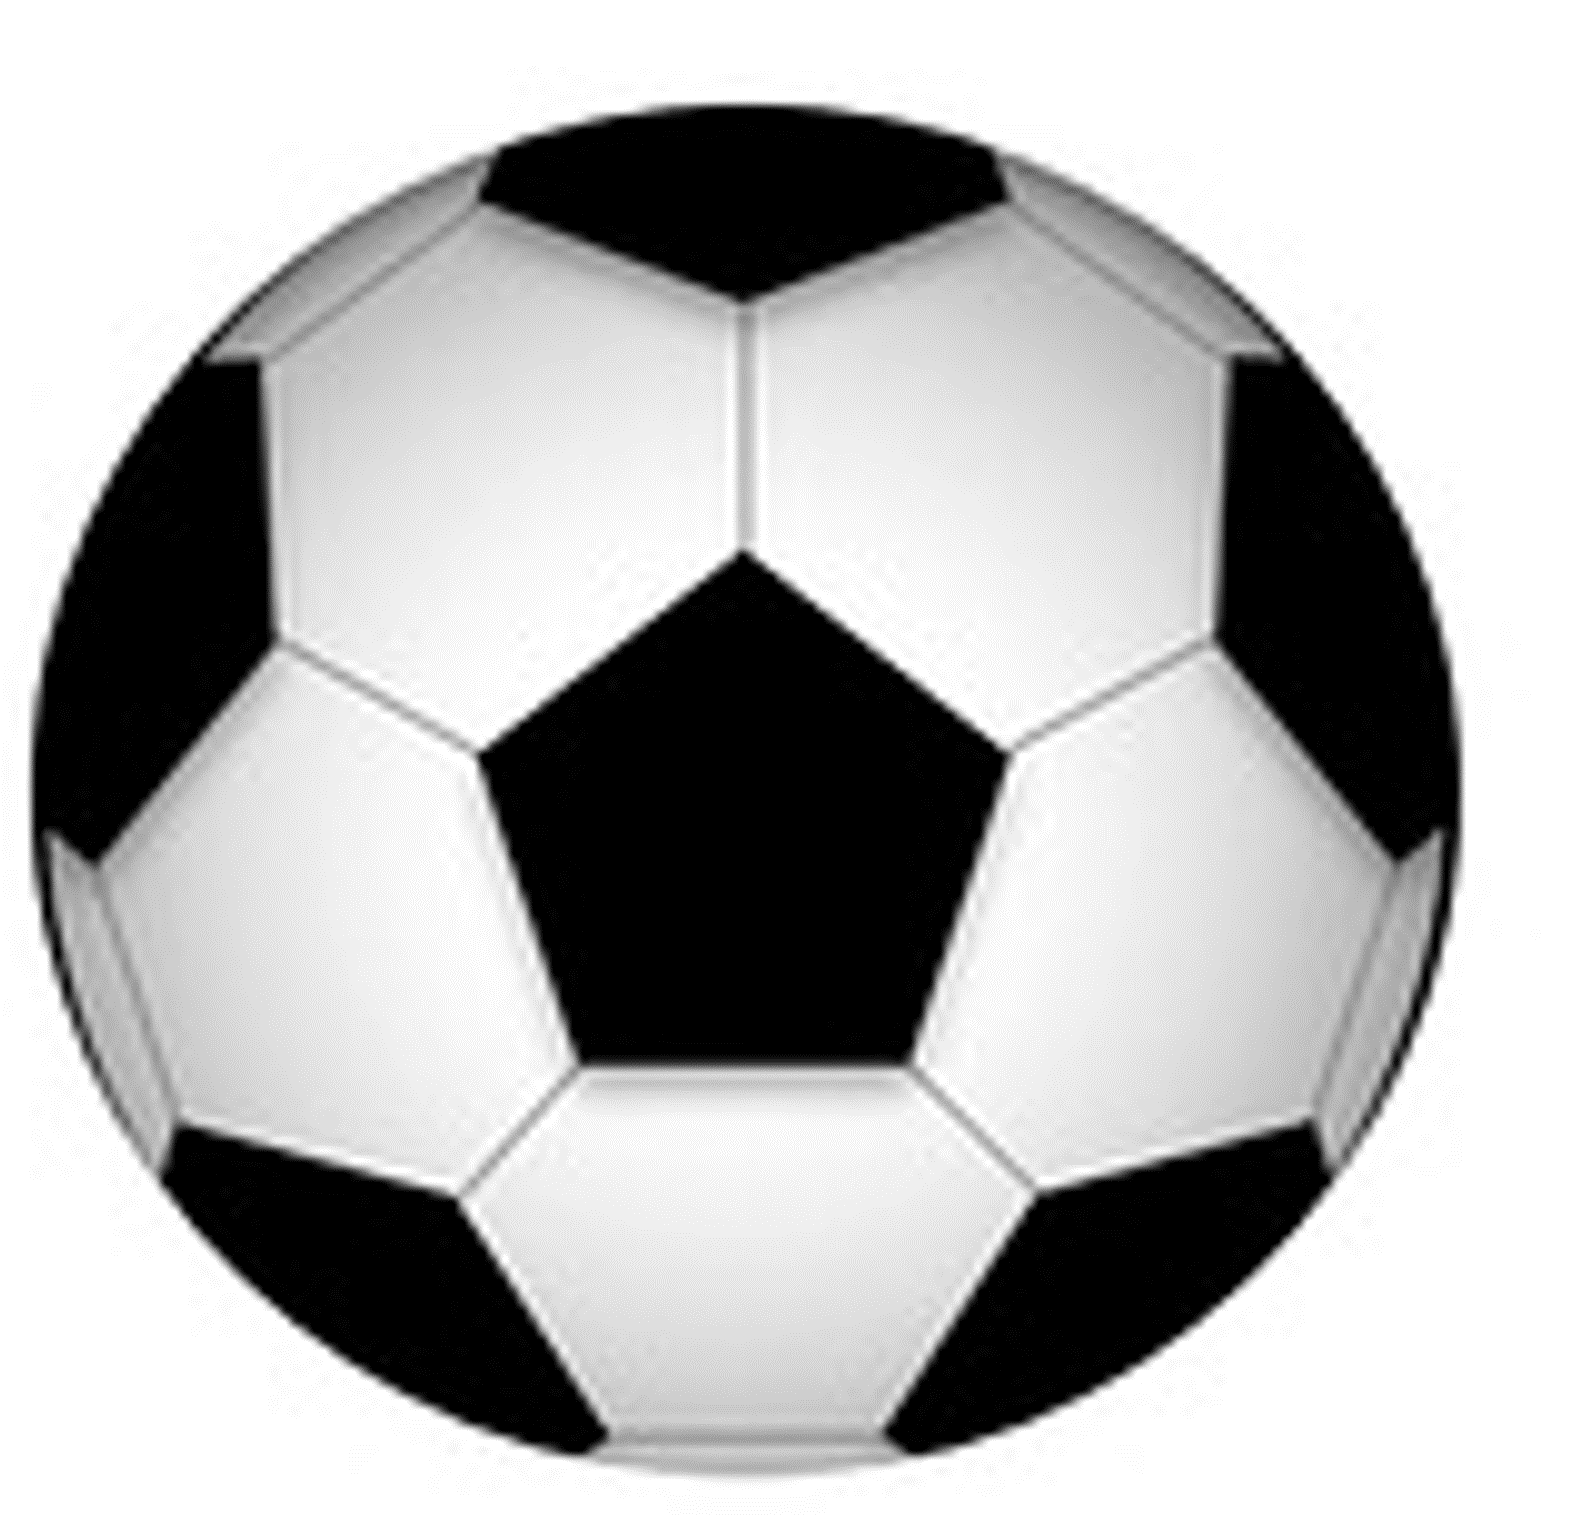
\includegraphics[width=1cm, height=1cm]{C6M17 - DT - Q5.png}  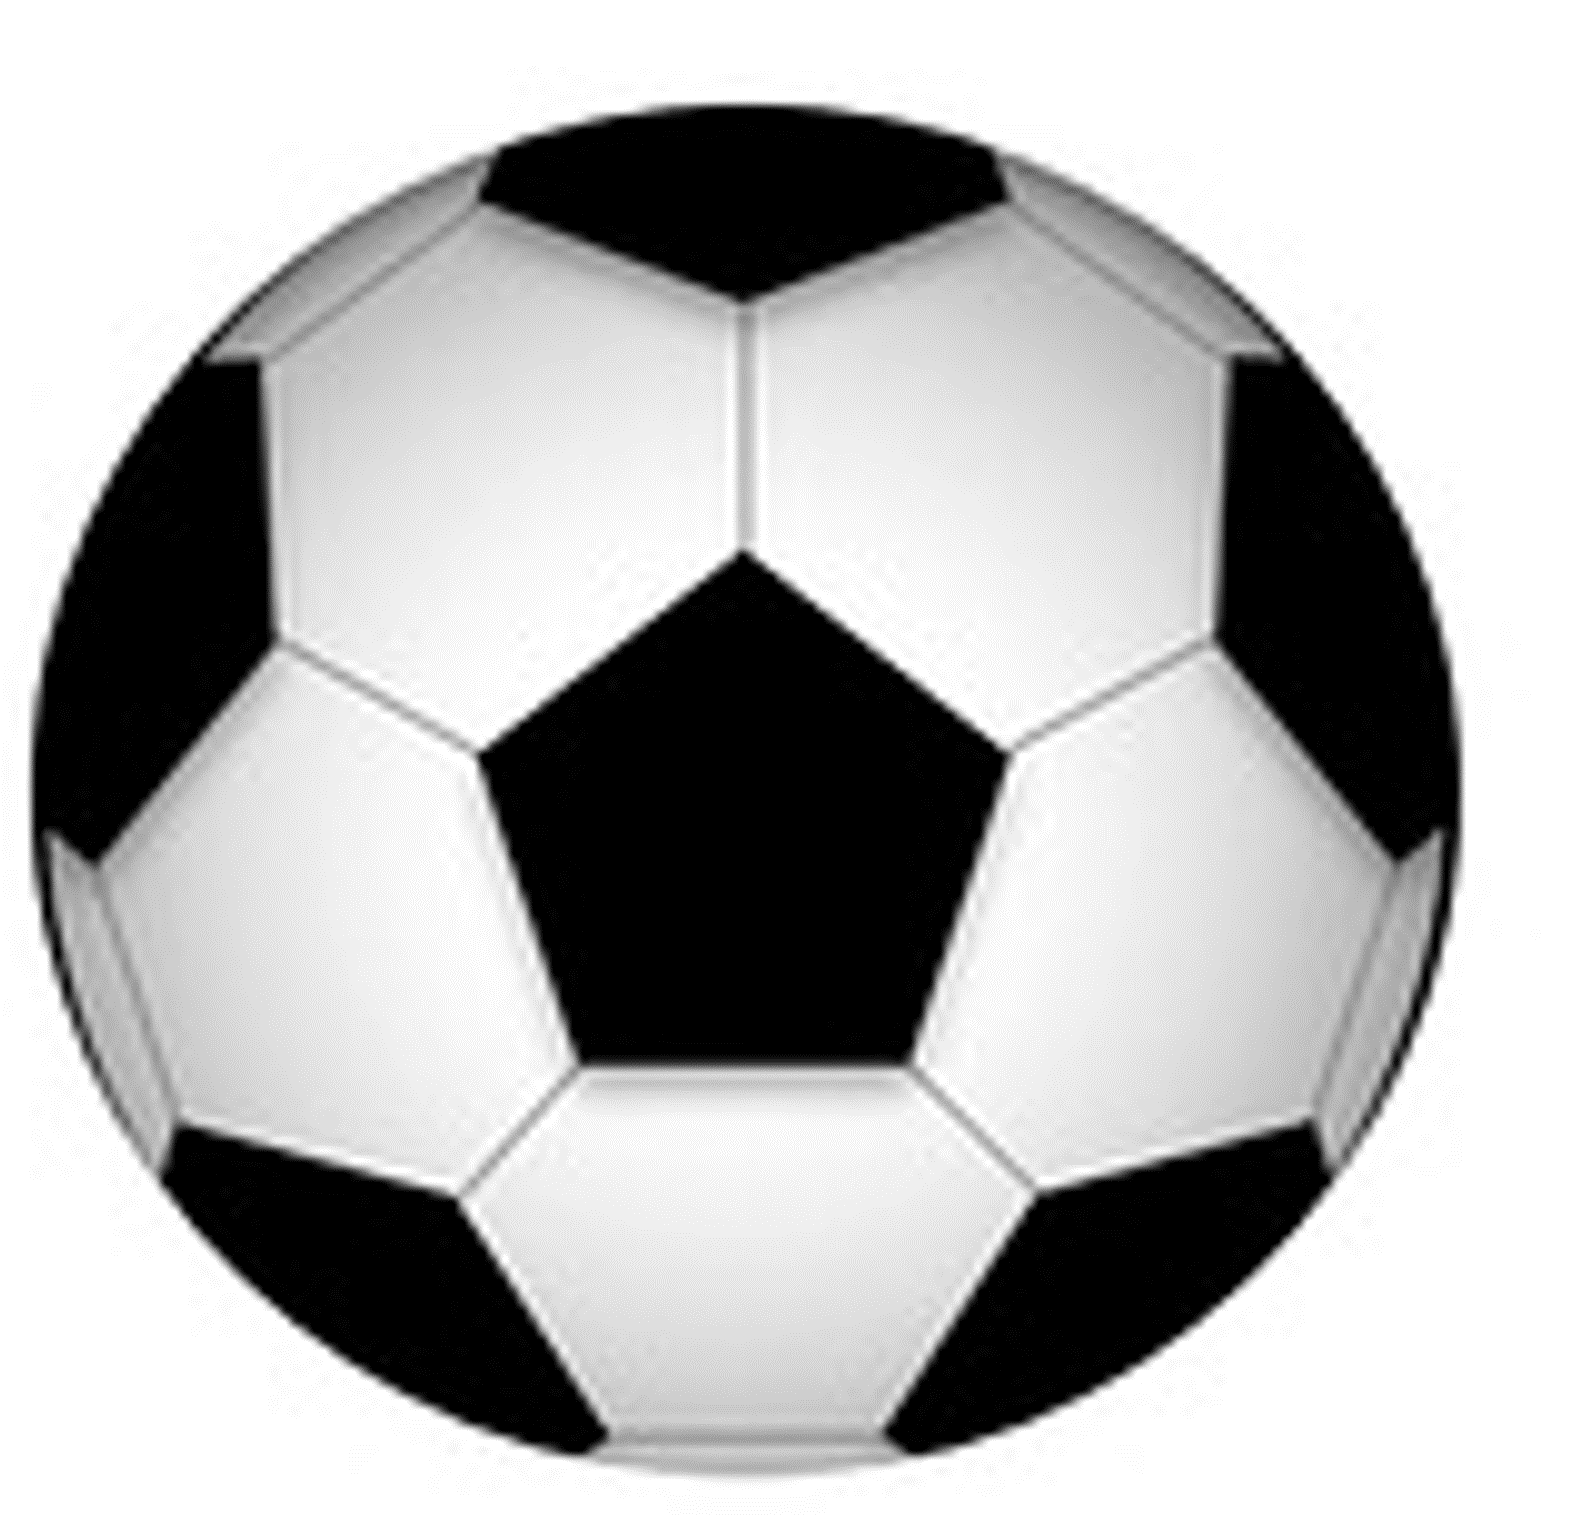
\includegraphics[width=1cm, height=1cm]{C6M17 - DT - Q5.png} 
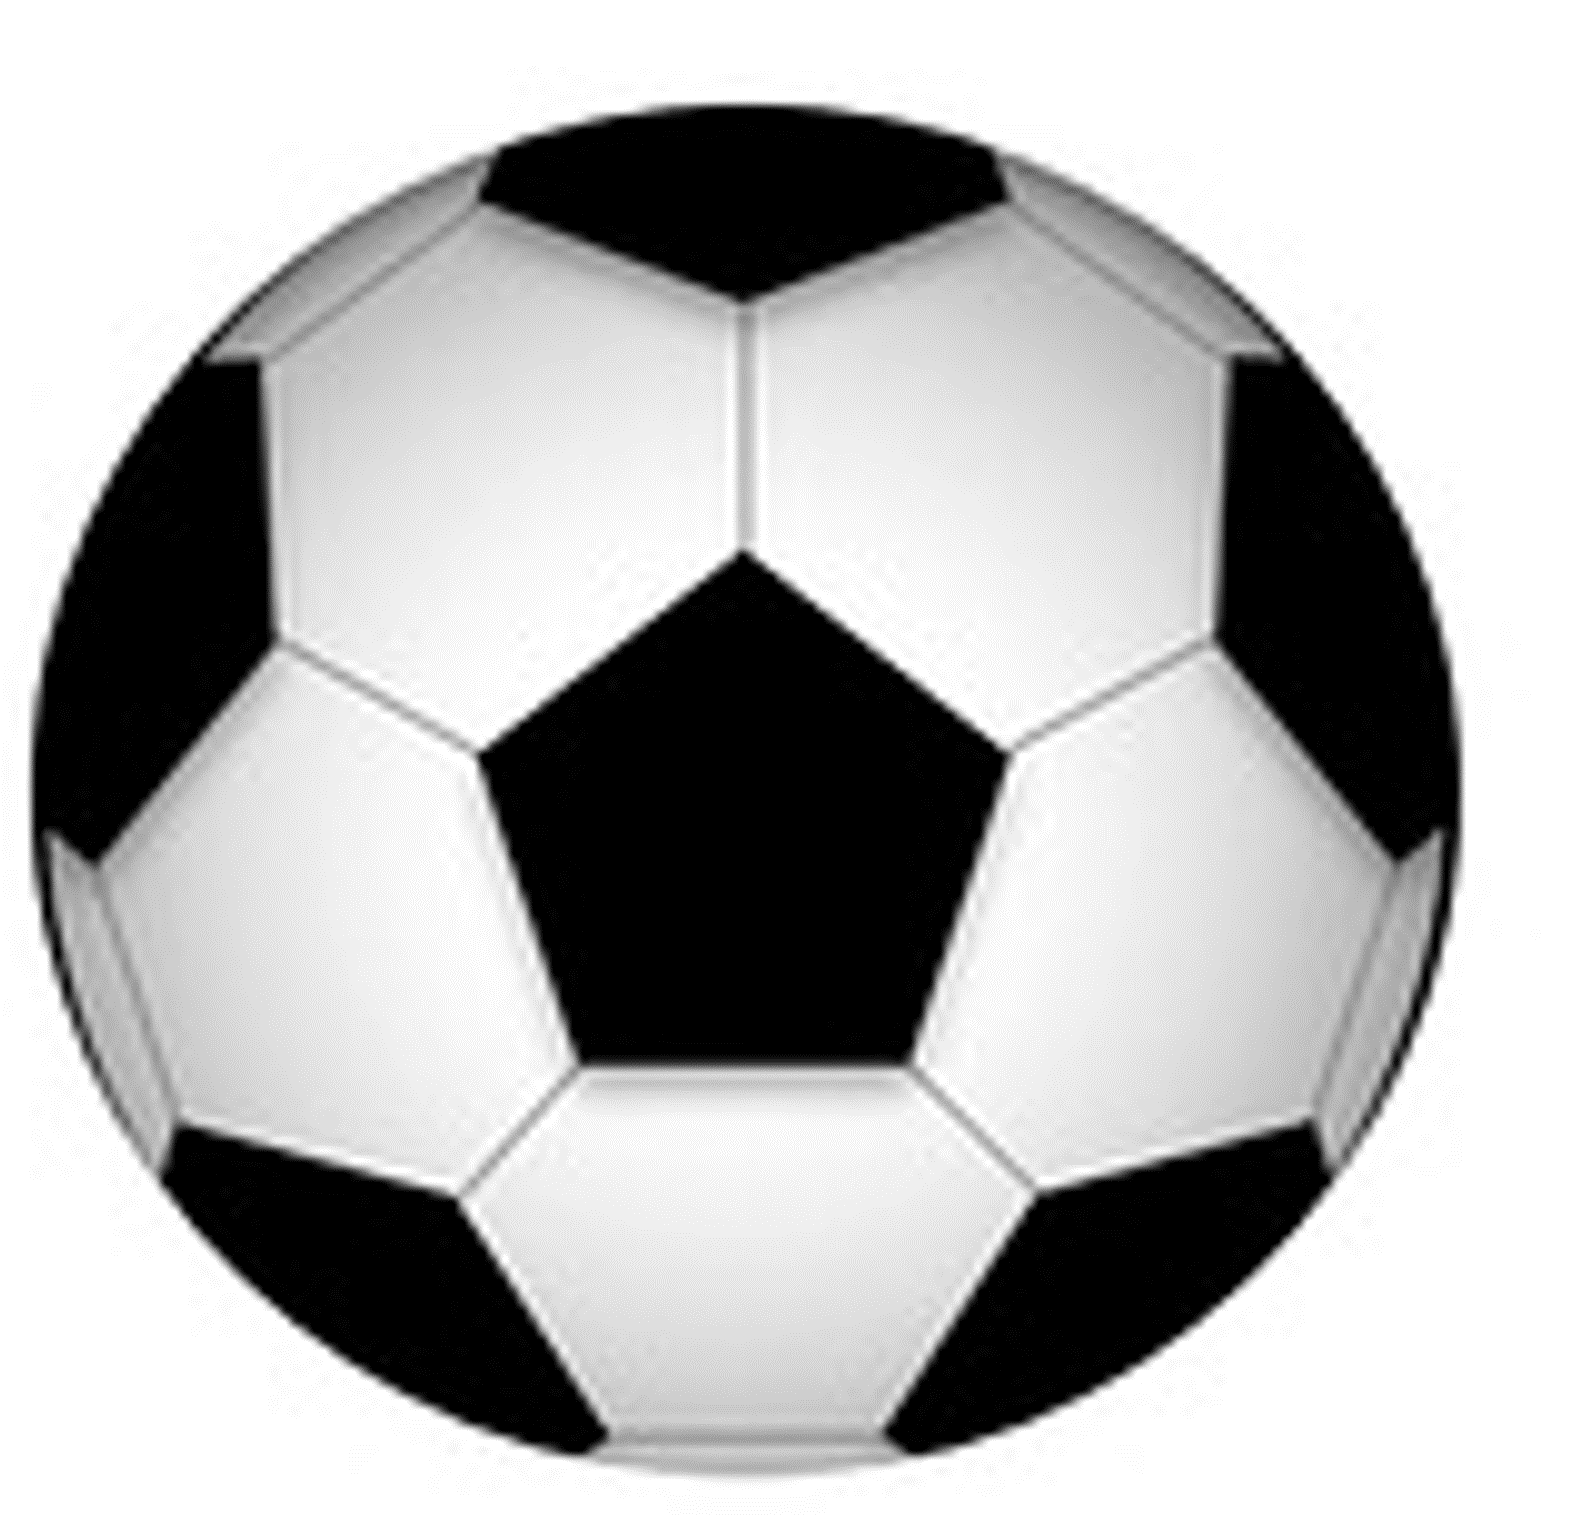
\includegraphics[width=1cm, height=1cm]{C6M17 - DT - Q5.png} 
},
optionC={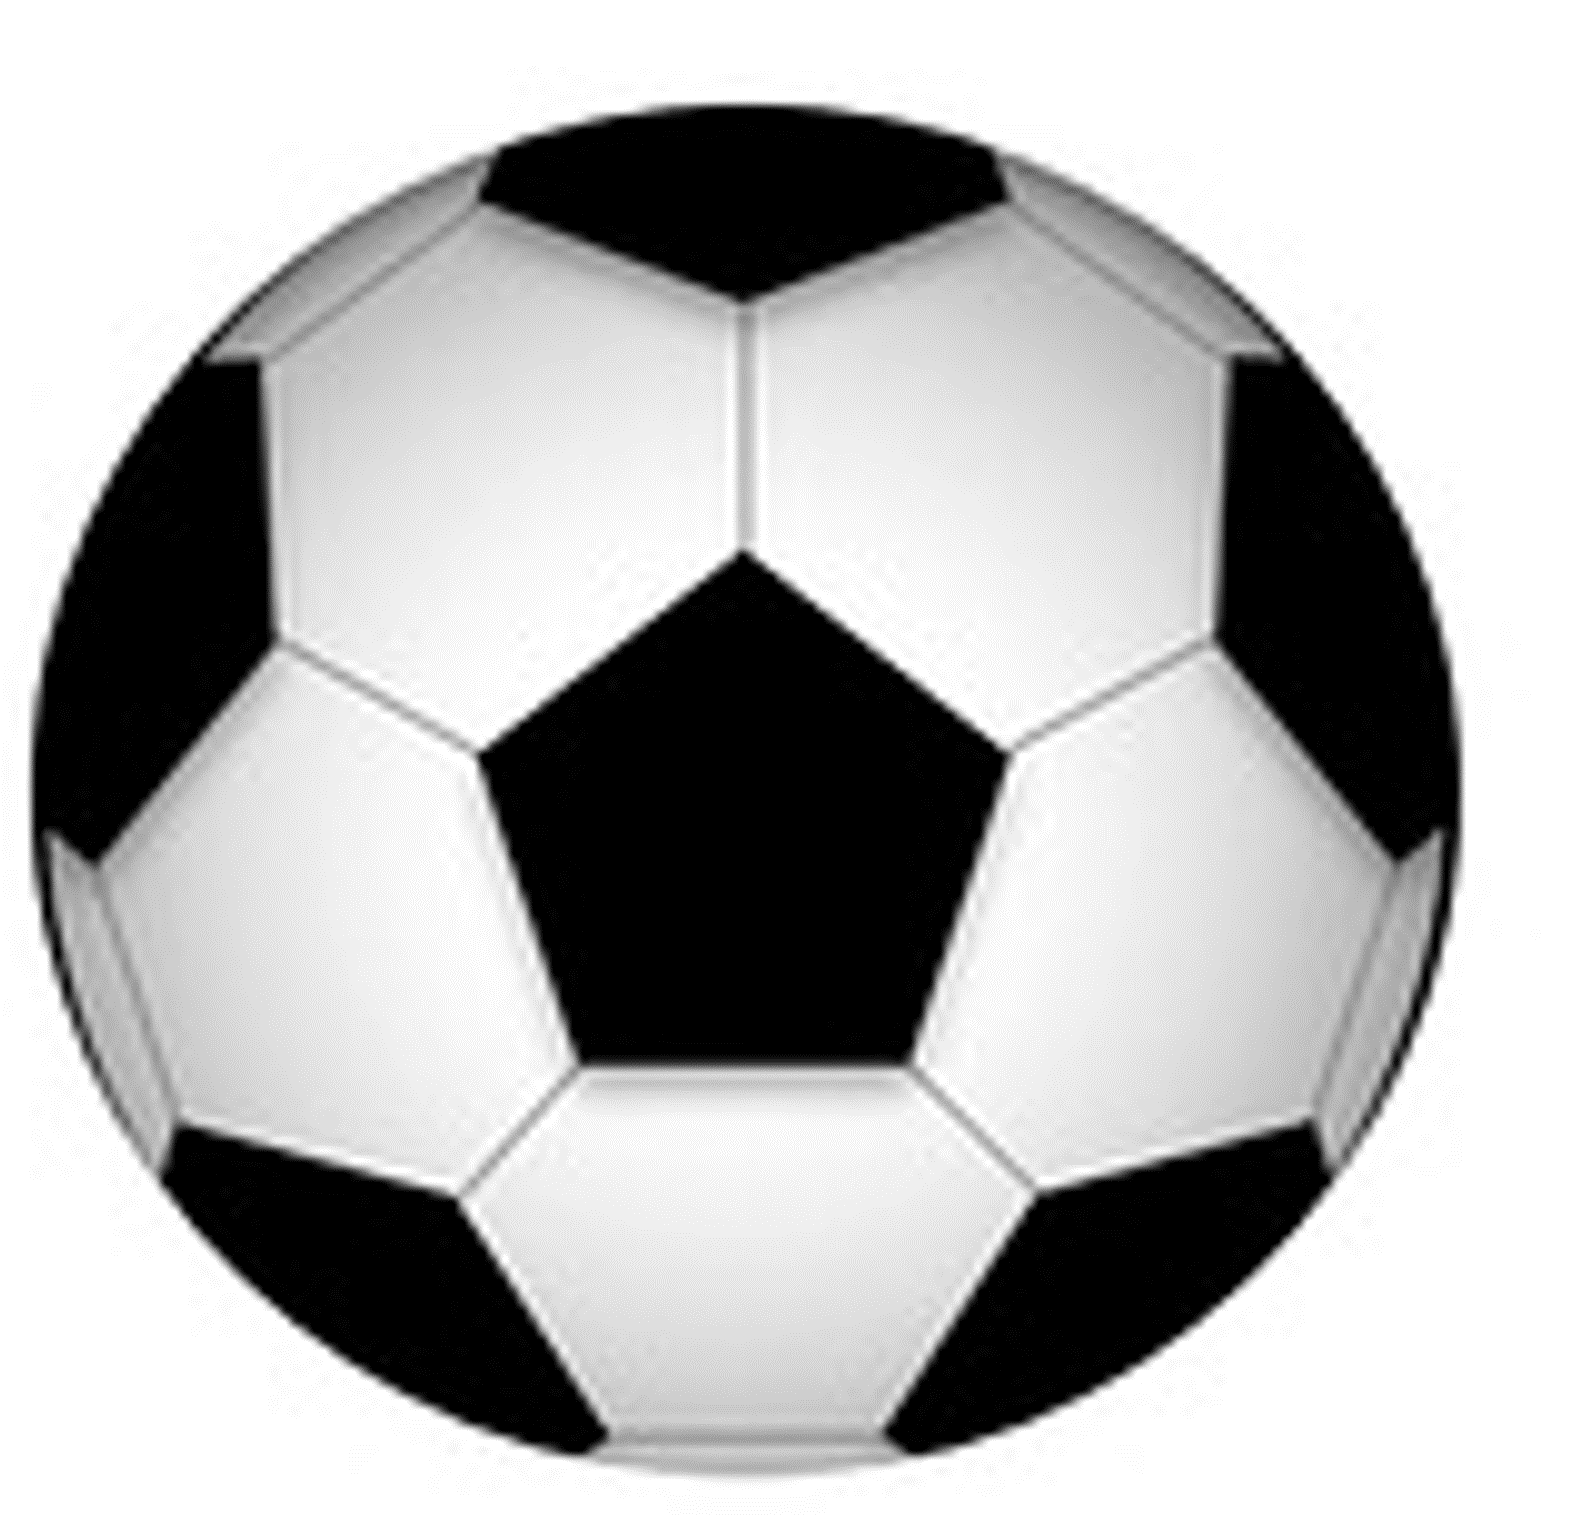
\includegraphics[width=1cm, height=1cm]{C6M17 - DT - Q5.png}
},
optionD={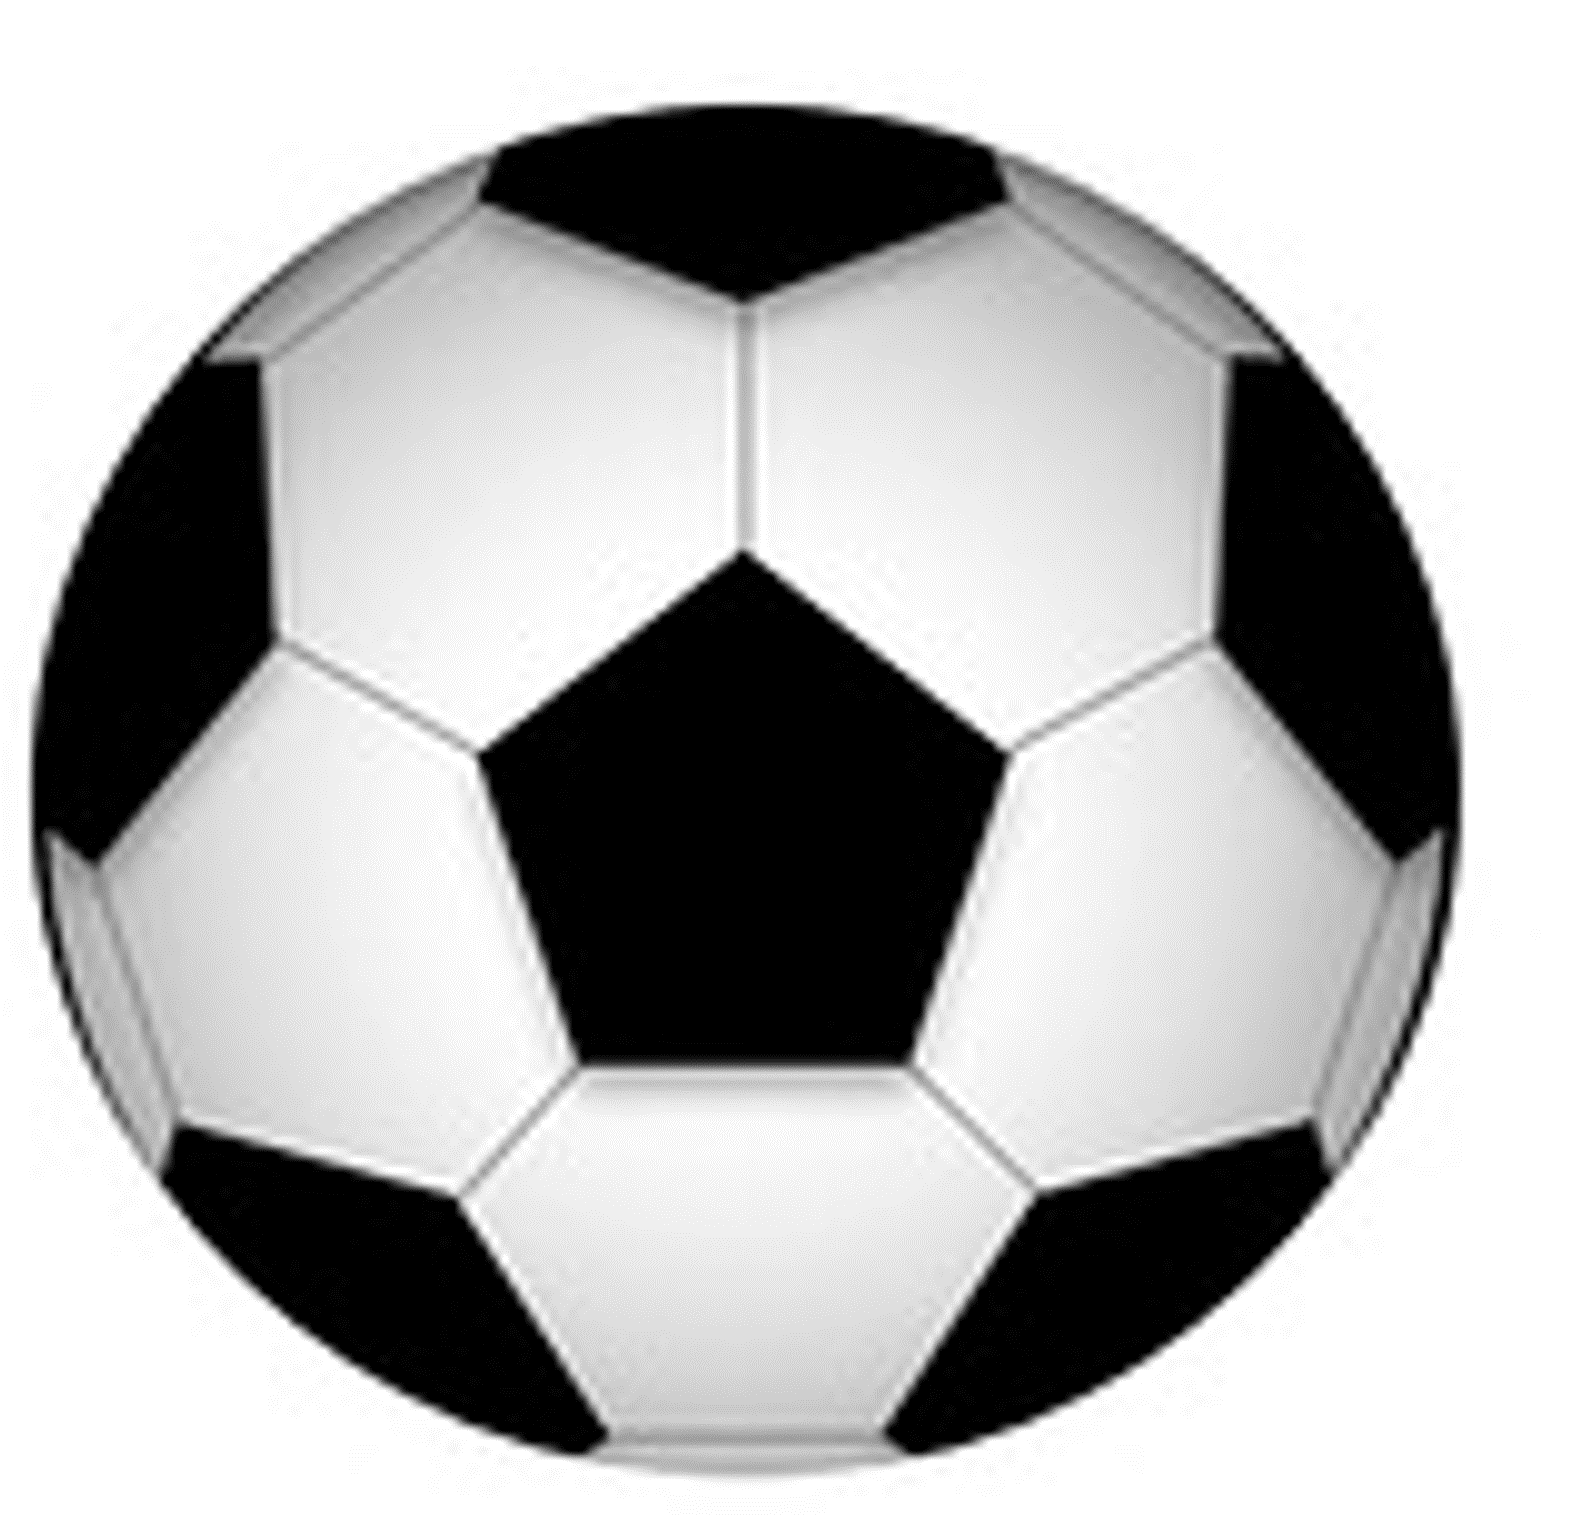
\includegraphics[width=1cm, height=1cm]{C6M17 - DT - Q5.png}
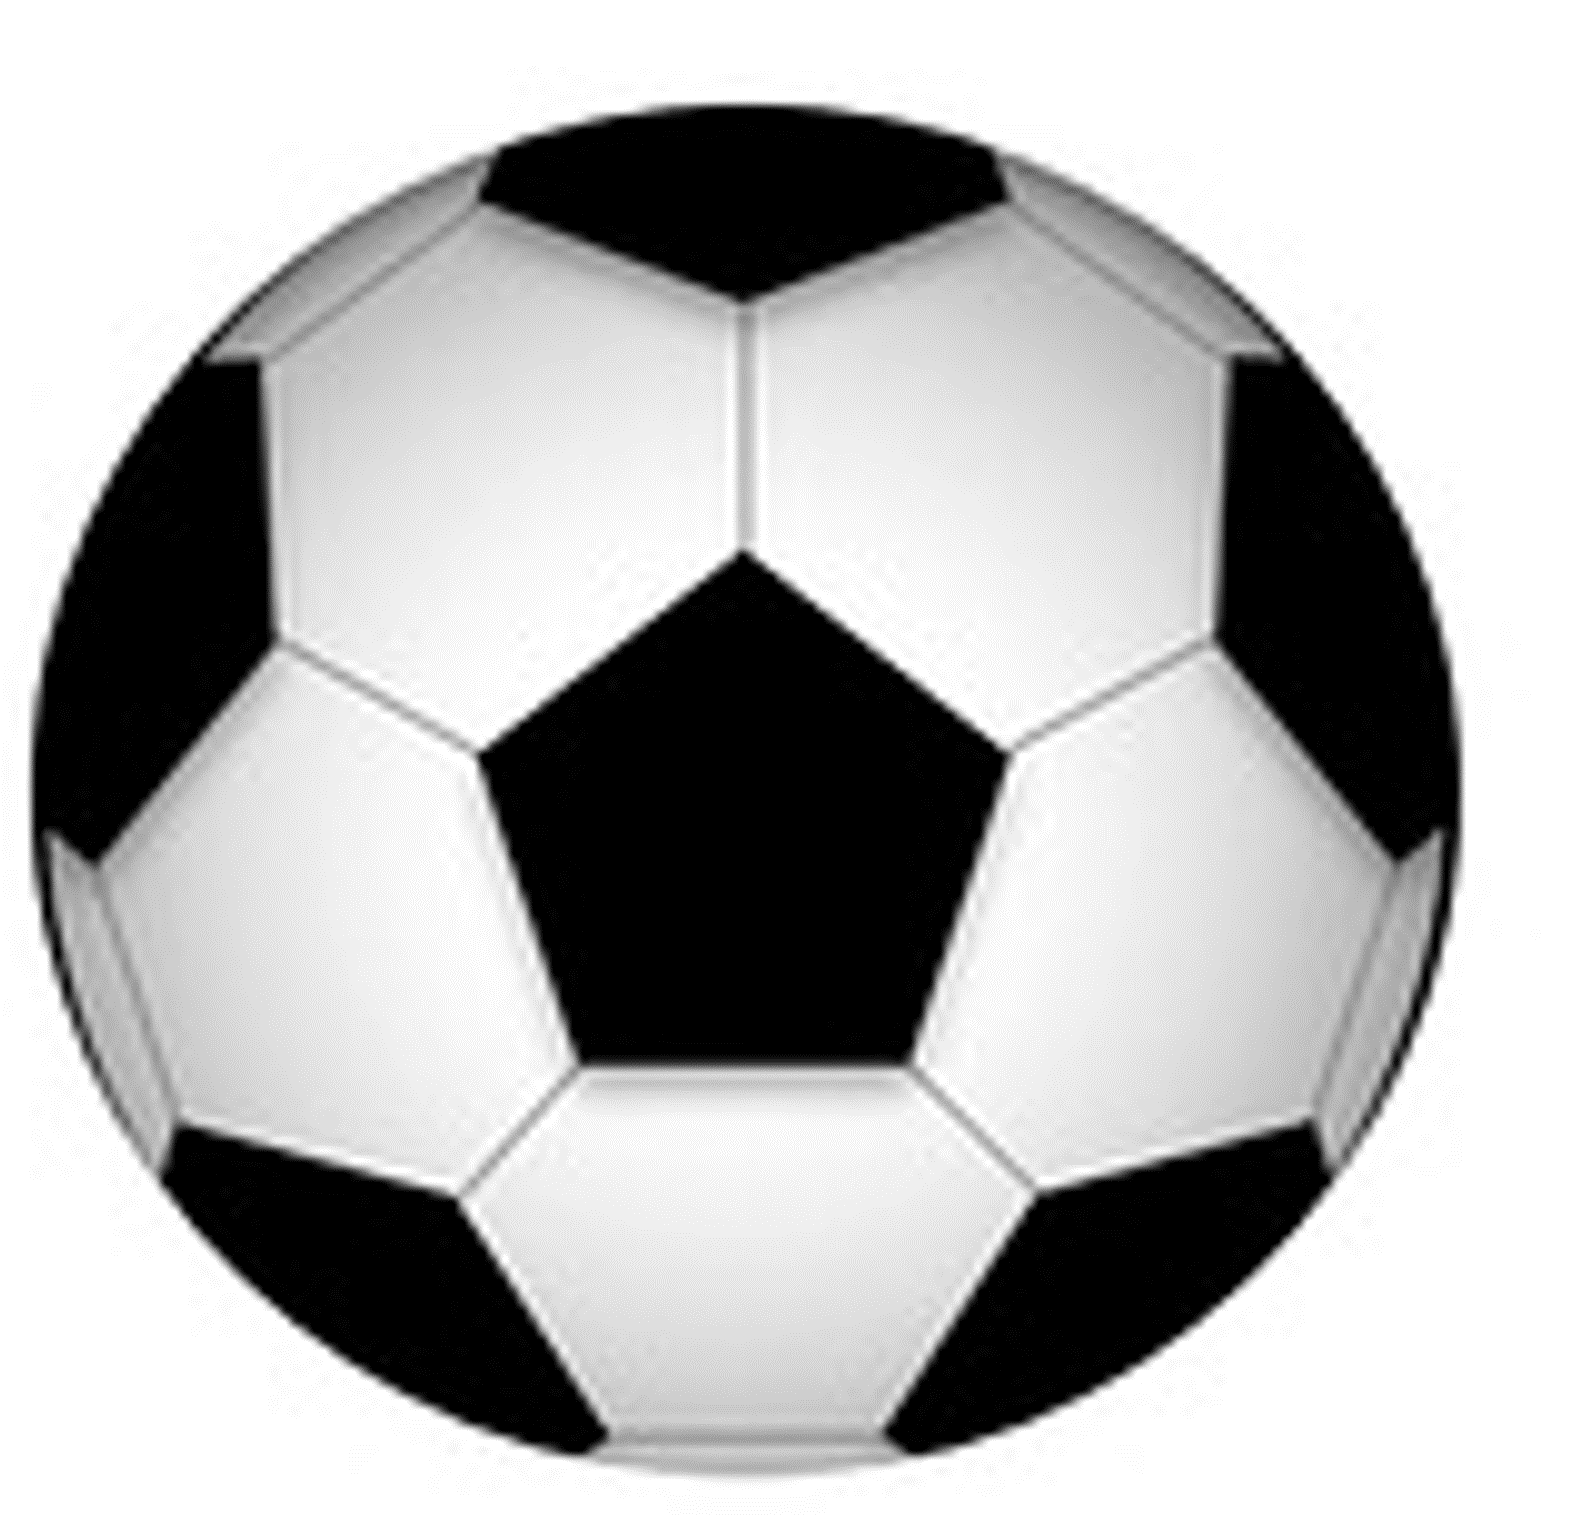
\includegraphics[width=1cm, height=1cm]{C6M17 - DT - Q5.png}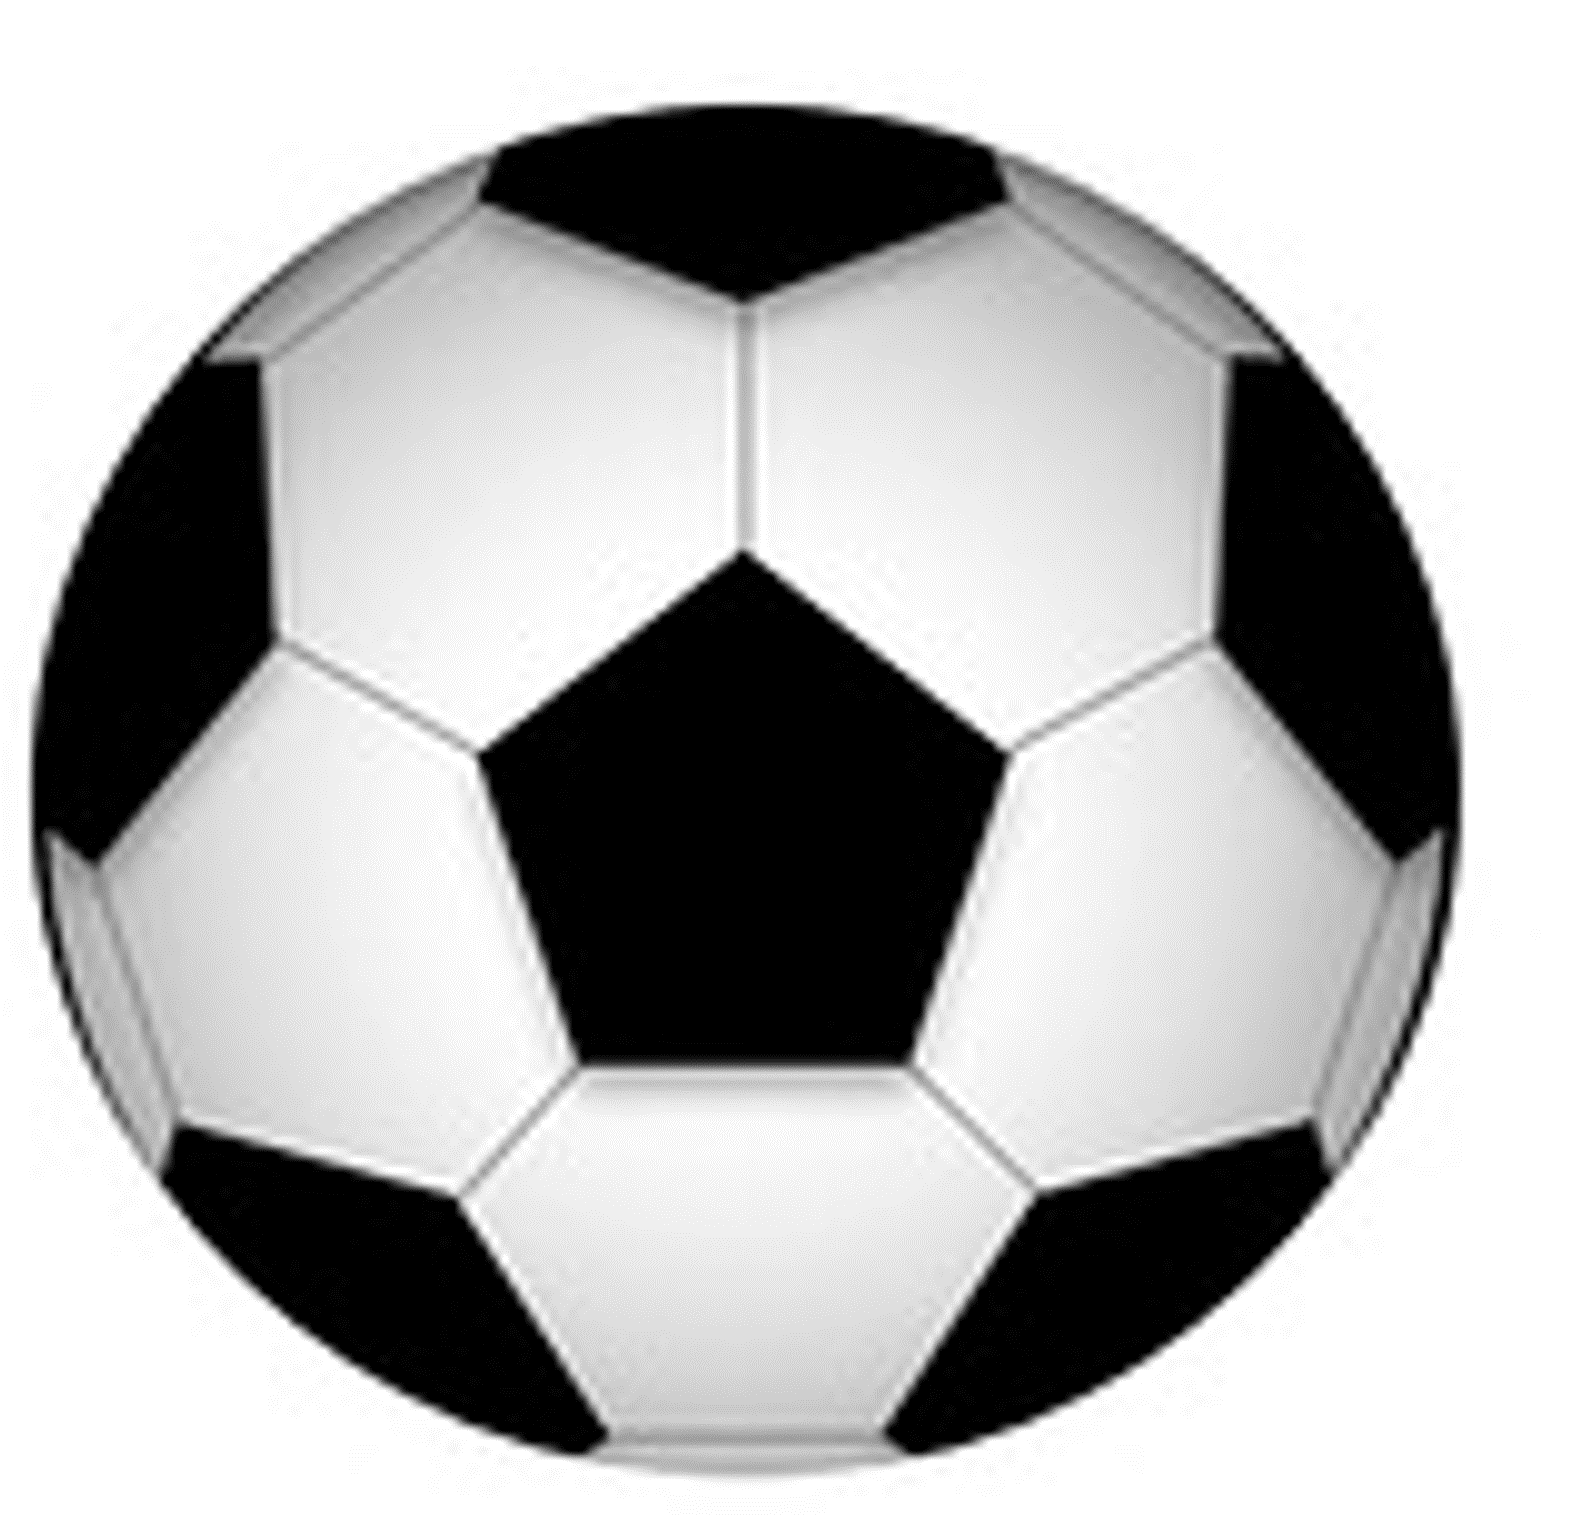
\includegraphics[width=1cm, height=1cm]{C6M17 - DT - Q5.png}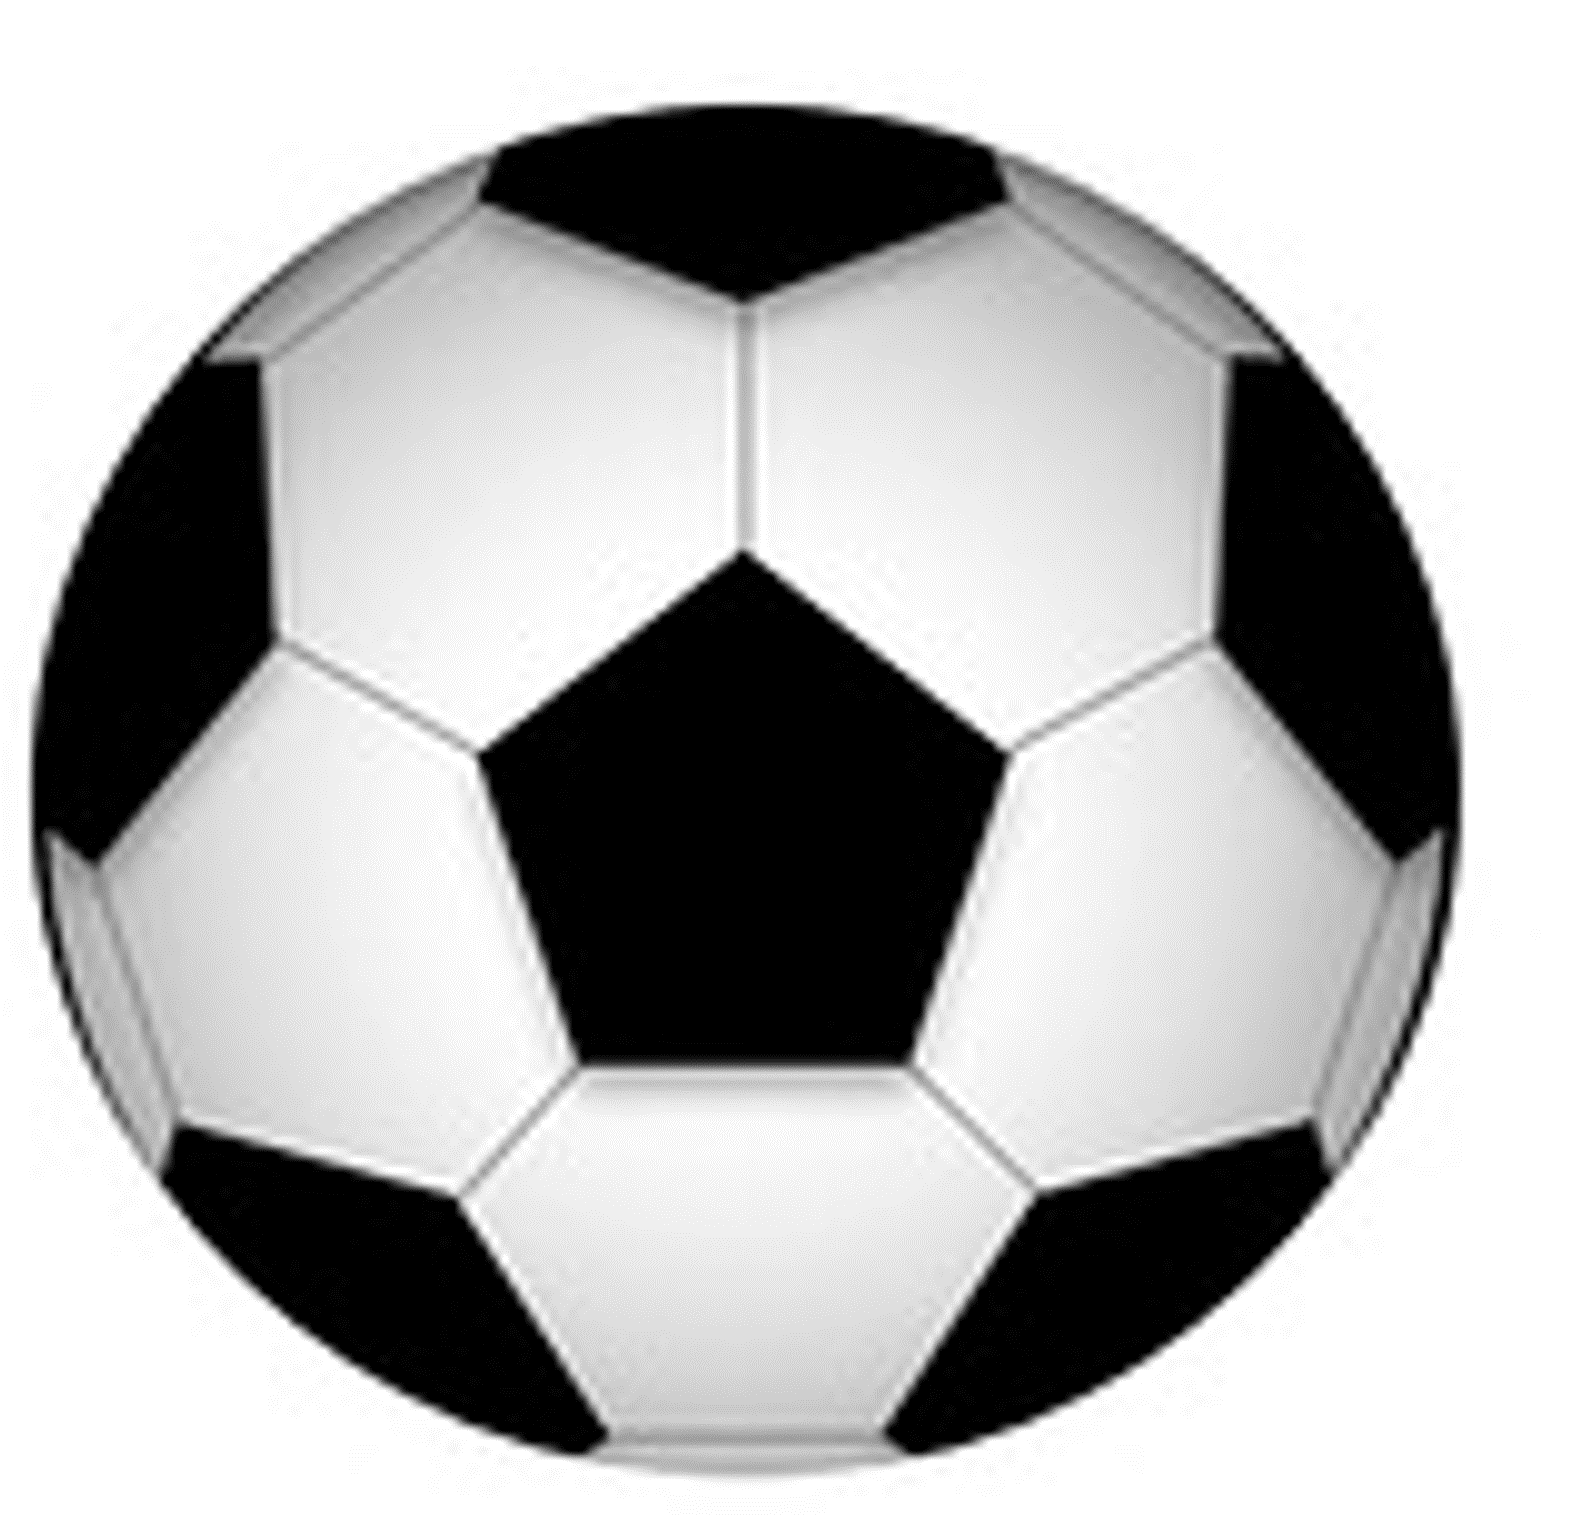
\includegraphics[width=1cm, height=1cm]{C6M17 - DT - Q5.png}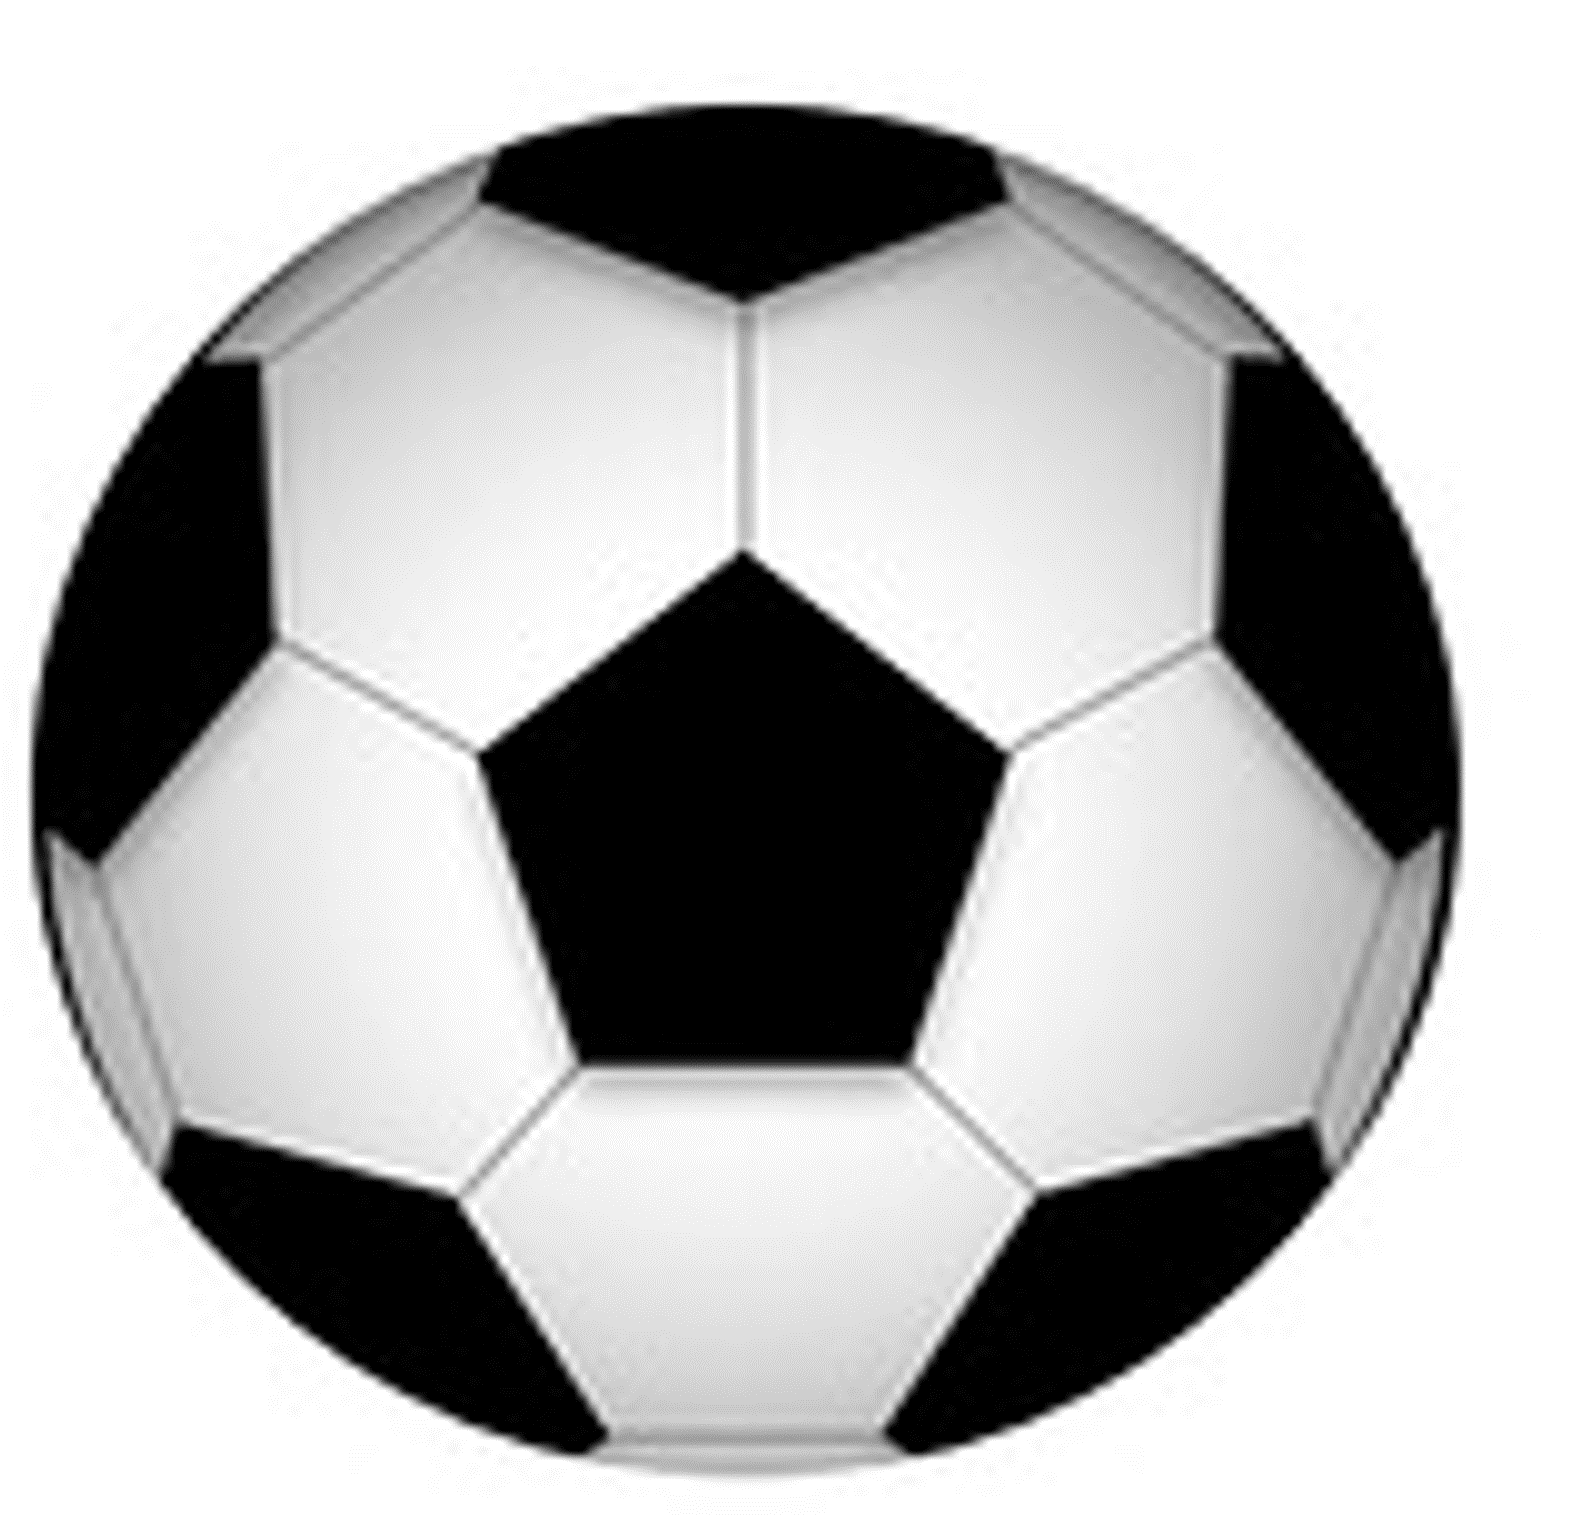
\includegraphics[width=1cm, height=1cm]{C6M17 - DT - Q5.png}
},
leftmini={0.35},
rightmini={0.4},
correctoption={D},
}
% end-of-question

%-----------------------------------------------------------
%                        Question [  ]
%-----------------------------------------------------------
% start-of-question
\mcqimgleftFourOne{
questionnumber={6}, 
questionTag={C6M17 – DT – Q6}, 
questiontext={Represent the given number of trees in tally marks.},
imgtabletikz = { 

\includegraphics[width=2cm, height=2.5cm]{C6M17 - DT - Q6.png}
\includegraphics[width=2cm, height=2.5cm]{C6M17 - DT - Q6.png}
\includegraphics[width=2cm, height=2.5cm]{C6M17 - DT - Q6.png}
\includegraphics[width=2cm, height=2.5cm]{C6M17 - DT - Q6.png}
\includegraphics[width=2cm, height=2.5cm]{C6M17 - DT - Q6.png} },
optionA={
\tikzset{every picture/.style={line width=0.75pt}} 
\begin{tikzpicture}[x=0.75pt,y=0.75pt,yscale=-1,xscale=1]
\draw    (102.33,50.14) -- (102.33,72.39) ;
\draw    (114.28,50) -- (114.28,72.25) ;
\draw    (125.36,50.28) -- (125.36,72.53) ;
\draw    (137.31,50.42) -- (137.31,72.67) ;
\draw    (125.36,50.28) -- (102.33,72.39) ;
\draw    (148.31,50.42) -- (148.31,72.67) ;
\end{tikzpicture}
},
optionB={ 
\tikzset{every picture/.style={line width=0.75pt}} 
\begin{tikzpicture}[x=0.75pt,y=0.75pt,yscale=-1,xscale=1]
\draw    (100.31,116.42) -- (100.31,138.67) ;
\draw    (112.26,116) -- (112.26,138.25) ;
\draw    (123.33,116.14) -- (123.33,138.39) ;
\draw    (133.26,115.95) -- (133.26,138.19) ;
\end{tikzpicture}
},
optionC={   
\tikzset{every picture/.style={line width=0.75pt}} 
\begin{tikzpicture}[x=0.75pt,y=0.75pt,yscale=-1,xscale=1]
\draw    (276.33,114.14) -- (276.33,136.39) ;
\draw    (288.28,114) -- (288.28,136.25) ;
\draw    (299.36,114.28) -- (299.36,136.53) ;
\draw    (311.31,114.42) -- (311.31,136.67) ;
\draw    (293.28,114) -- (270.28,136) ;
\draw    (323.26,114) -- (323.26,136.25) ;
\draw    (334.33,114.14) -- (334.33,136.39) ;
\draw    (344.26,113.95) -- (344.26,136.19) ;
\draw    (355.33,114.09) -- (355.33,136.33) ;
\draw    (316.28,116) -- (293.28,138) ;
\draw    (338.48,115) -- (315.48,137) ;
\draw    (360.33,114.39) -- (337.33,136.39) ;
\draw    (366.06,113.2) -- (366.06,135.45) ;
\draw    (377.13,113.34) -- (377.13,135.59) ;
\draw    (381.28,114.2) -- (358.28,136.2) ;
\end{tikzpicture}
},
optionD={
\tikzset{every picture/.style={line width=0.75pt}} 
\begin{tikzpicture}[x=0.75pt,y=0.75pt,yscale=-1,xscale=1]
\draw    (98.33,161.14) -- (98.33,183.39) ;
\draw    (110.28,161) -- (110.28,183.25) ;
\draw    (121.36,161.28) -- (121.36,183.53) ;
\draw    (133.31,161.42) -- (133.31,183.67) ;
\draw    (133.31,161.42) -- (98.33,183.39) ;
\end{tikzpicture}
},
correctoption={D},
leftmini={0.5},
rightmini={0.4}
}
% end-of-question


%-----------------------------------------------------------
%                        Question [ ]
%-----------------------------------------------------------
% start-of-question
\mcqimgleftFourOne{
questionnumber={7}, 
questionTag={C6M17 – DT – Q7}, 
questiontext={Observe the given pictograph and find the total number of torch lights sold on Tuesday and Thursday.},
imgtabletikz  = {
\renewcommand{\arraystretch}{1.25}
\begin{tabular}{|c|c|}
\hline
  Days & Number of torch lights sold ($\infty$  = 2 torch lights) \\
  \hline
  Monday& $\infty$ \hspace{0.2cm} $\infty$ \hspace{0.2cm} $\infty$ \hspace{0.2cm} $\infty$ \hspace{0.2cm} $\infty$ \hspace{0.2cm} $\infty$  \hspace{0.2cm} $\infty$  \\
  \hline
  Tuesday  & $\infty$ \hspace{0.2cm} $\infty$ \hspace{0.2cm} $\infty$ \hspace{0.2cm}$\infty$ \hspace{0.2cm} $\infty$  \\
  \hline
  Wednesday & $\infty$ \hspace{0.2cm} $\infty$ \hspace{0.2cm} $\infty$ \hspace{0.2cm} $\infty$ \hspace{0.2cm} $\infty$ \hspace{0.2cm} $\infty$ \hspace{0.2cm} $\infty$ \hspace{0.2cm} $\infty$ \hspace{0.2cm} $\infty$ \\
  \hline
  Thursday & $\infty$ \hspace{0.2cm} $\infty$ \hspace{0.2cm} $\infty$ \hspace{0.2cm} $\infty$ \\
  \hline
\end{tabular}  },
optionA={9},
optionB={10},
optionC={18},
optionD={2},
leftmini={0.5},
rightmini={0.3},
correctoption={C},
}
% end-of-question

%-----------------------------------------------------------
%                        Question [  ]
%-----------------------------------------------------------
% start-of-question
\mcqimgleftFourOne{
questionnumber={8}, 
questionTag={C6M17 – DT – Q8}, 
questiontext={Find the day in which the least number of fruits are sold.},
imgtabletikz = { 
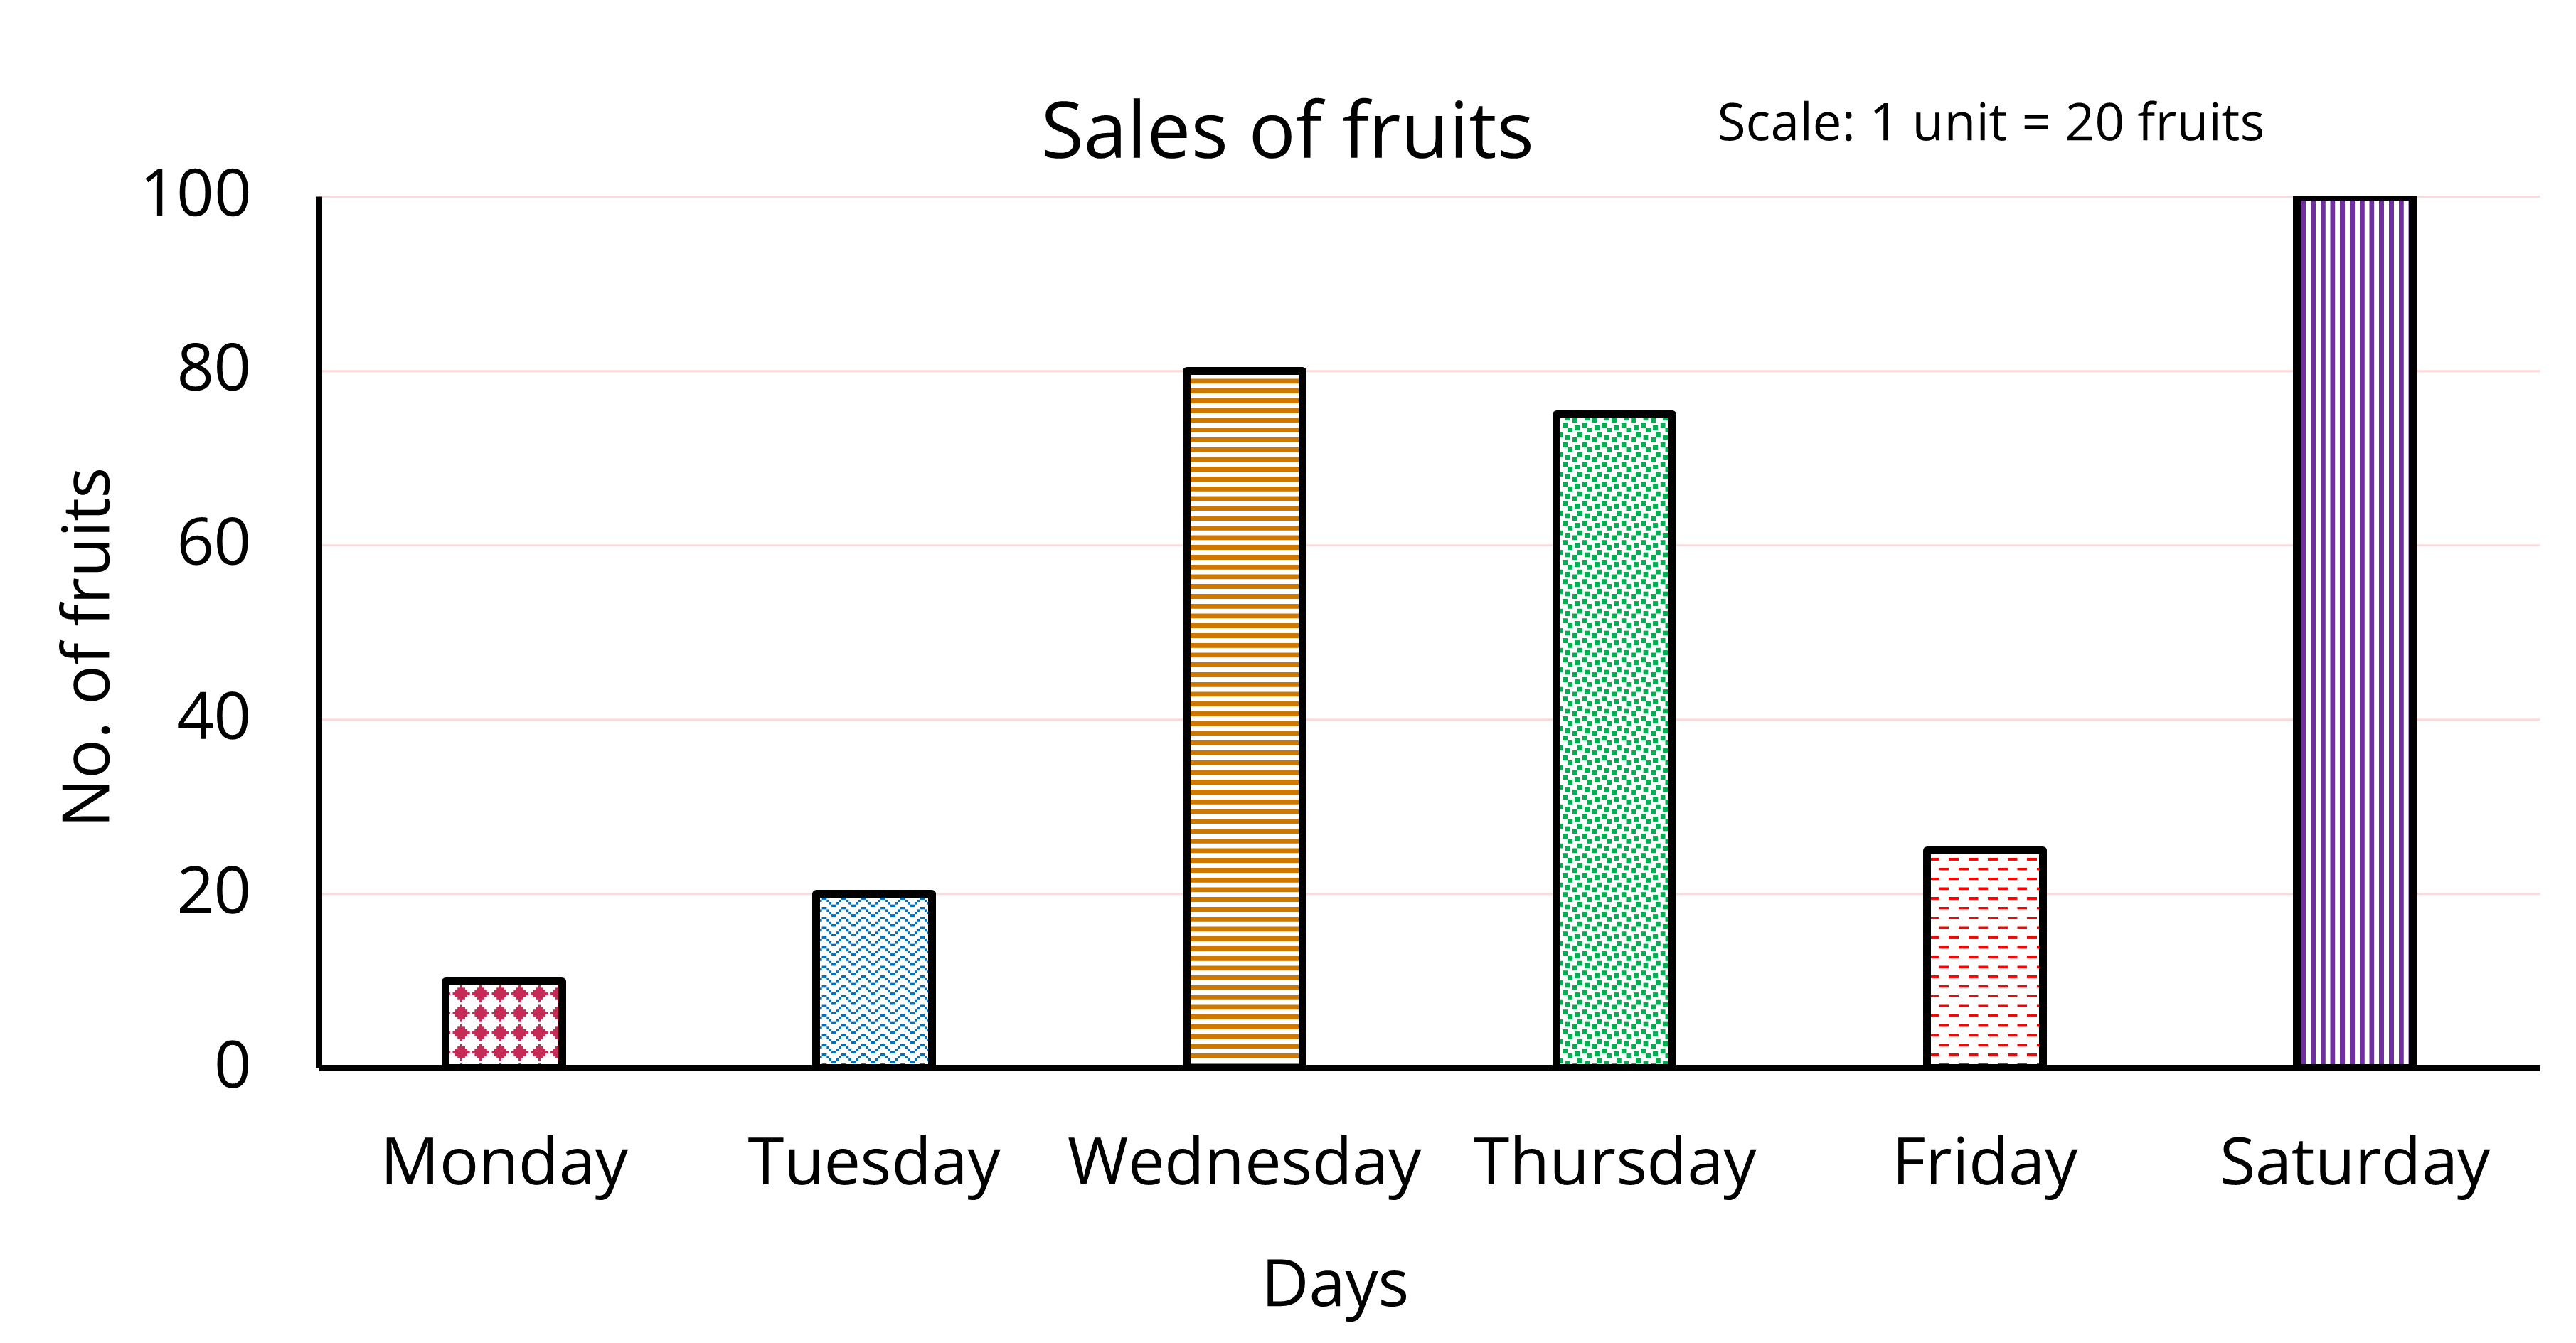
\includegraphics[width=13cm, height=6.5cm]{C6M17 - DT - Q3.png}},
optionA={Monday},
optionB={Wednesday},
optionC={Friday},
optionD={Saturday},
leftmini={0.65},
rightmini={0.25},
correctoption={A},
}
% end-of-question
%-----------------------------------------------------------
%                        Question [  ]
%-----------------------------------------------------------
% start-of-question
\mcqimgleftFourOne{
questionnumber={9}, 
questiontext={Observe the pictograph and complete them.},
questionTag={C6M17 – DT – Q9},
imgtabletikz = { 
\begin{table}[H]
\centering
\renewcommand{\arraystretch}{2.5}
\begin{tabular}{|p{5cm}|p{4cm}|}
\hline
Number of strawberries & Cost of strawberries\\
\hline
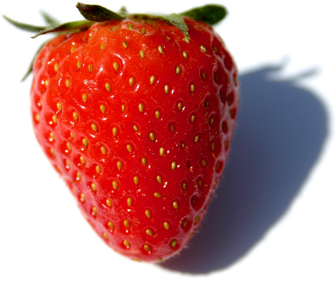
\includegraphics[width=1cm, height=0.8cm]{C6M17 - DT - Q9.png} & Rs. 15\\
\hline
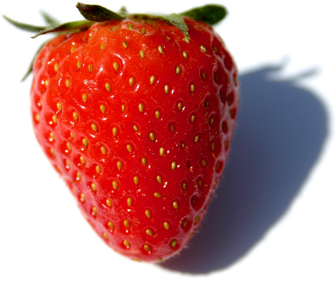
\includegraphics[width=1cm, height=0.8cm]{C6M17 - DT - Q9.png} 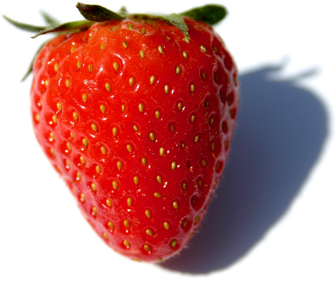
\includegraphics[width=1cm, height=0.8cm]{C6M17 - DT - Q9.png} 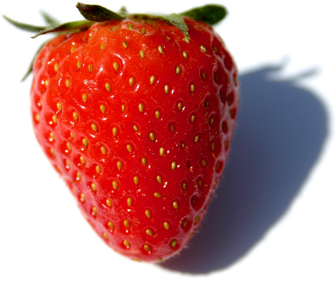
\includegraphics[width=1cm, height=0.8cm]{C6M17 - DT - Q9.png} 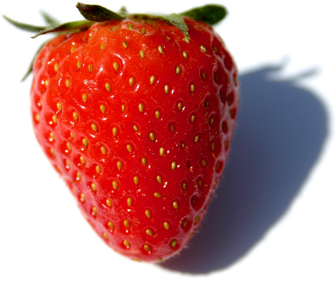
\includegraphics[width=1cm, height=0.8cm]{C6M17 - DT - Q9.png} & ? \\
\hline        
\end{tabular}
\end{table}
},
optionA={Rs. 60 },
optionB={Rs. 40 },
optionC={Rs. 4  },
optionD={Rs. 150},
leftmini={0.6},
rightmini={0.3},
correctoption={A},
}
% end-of-question

%-----------------------------------------------------------
%                        Question [48  ]
%-----------------------------------------------------------
% start-of-question
\mcqimgleftFourOne{
questionnumber={1}, 
questionTag={C6M06 – DT – Q1},
questiontext={If the price of the ball and bat are the same, what will be the lowest common multiple?},
imgtabletikz  = {
\tikzset{every picture/.style={line width=0.75pt}} 
\begin{tikzpicture}[x=0.75pt,y=0.75pt,yscale=-1,xscale=1]
\draw (223,66.16) node  {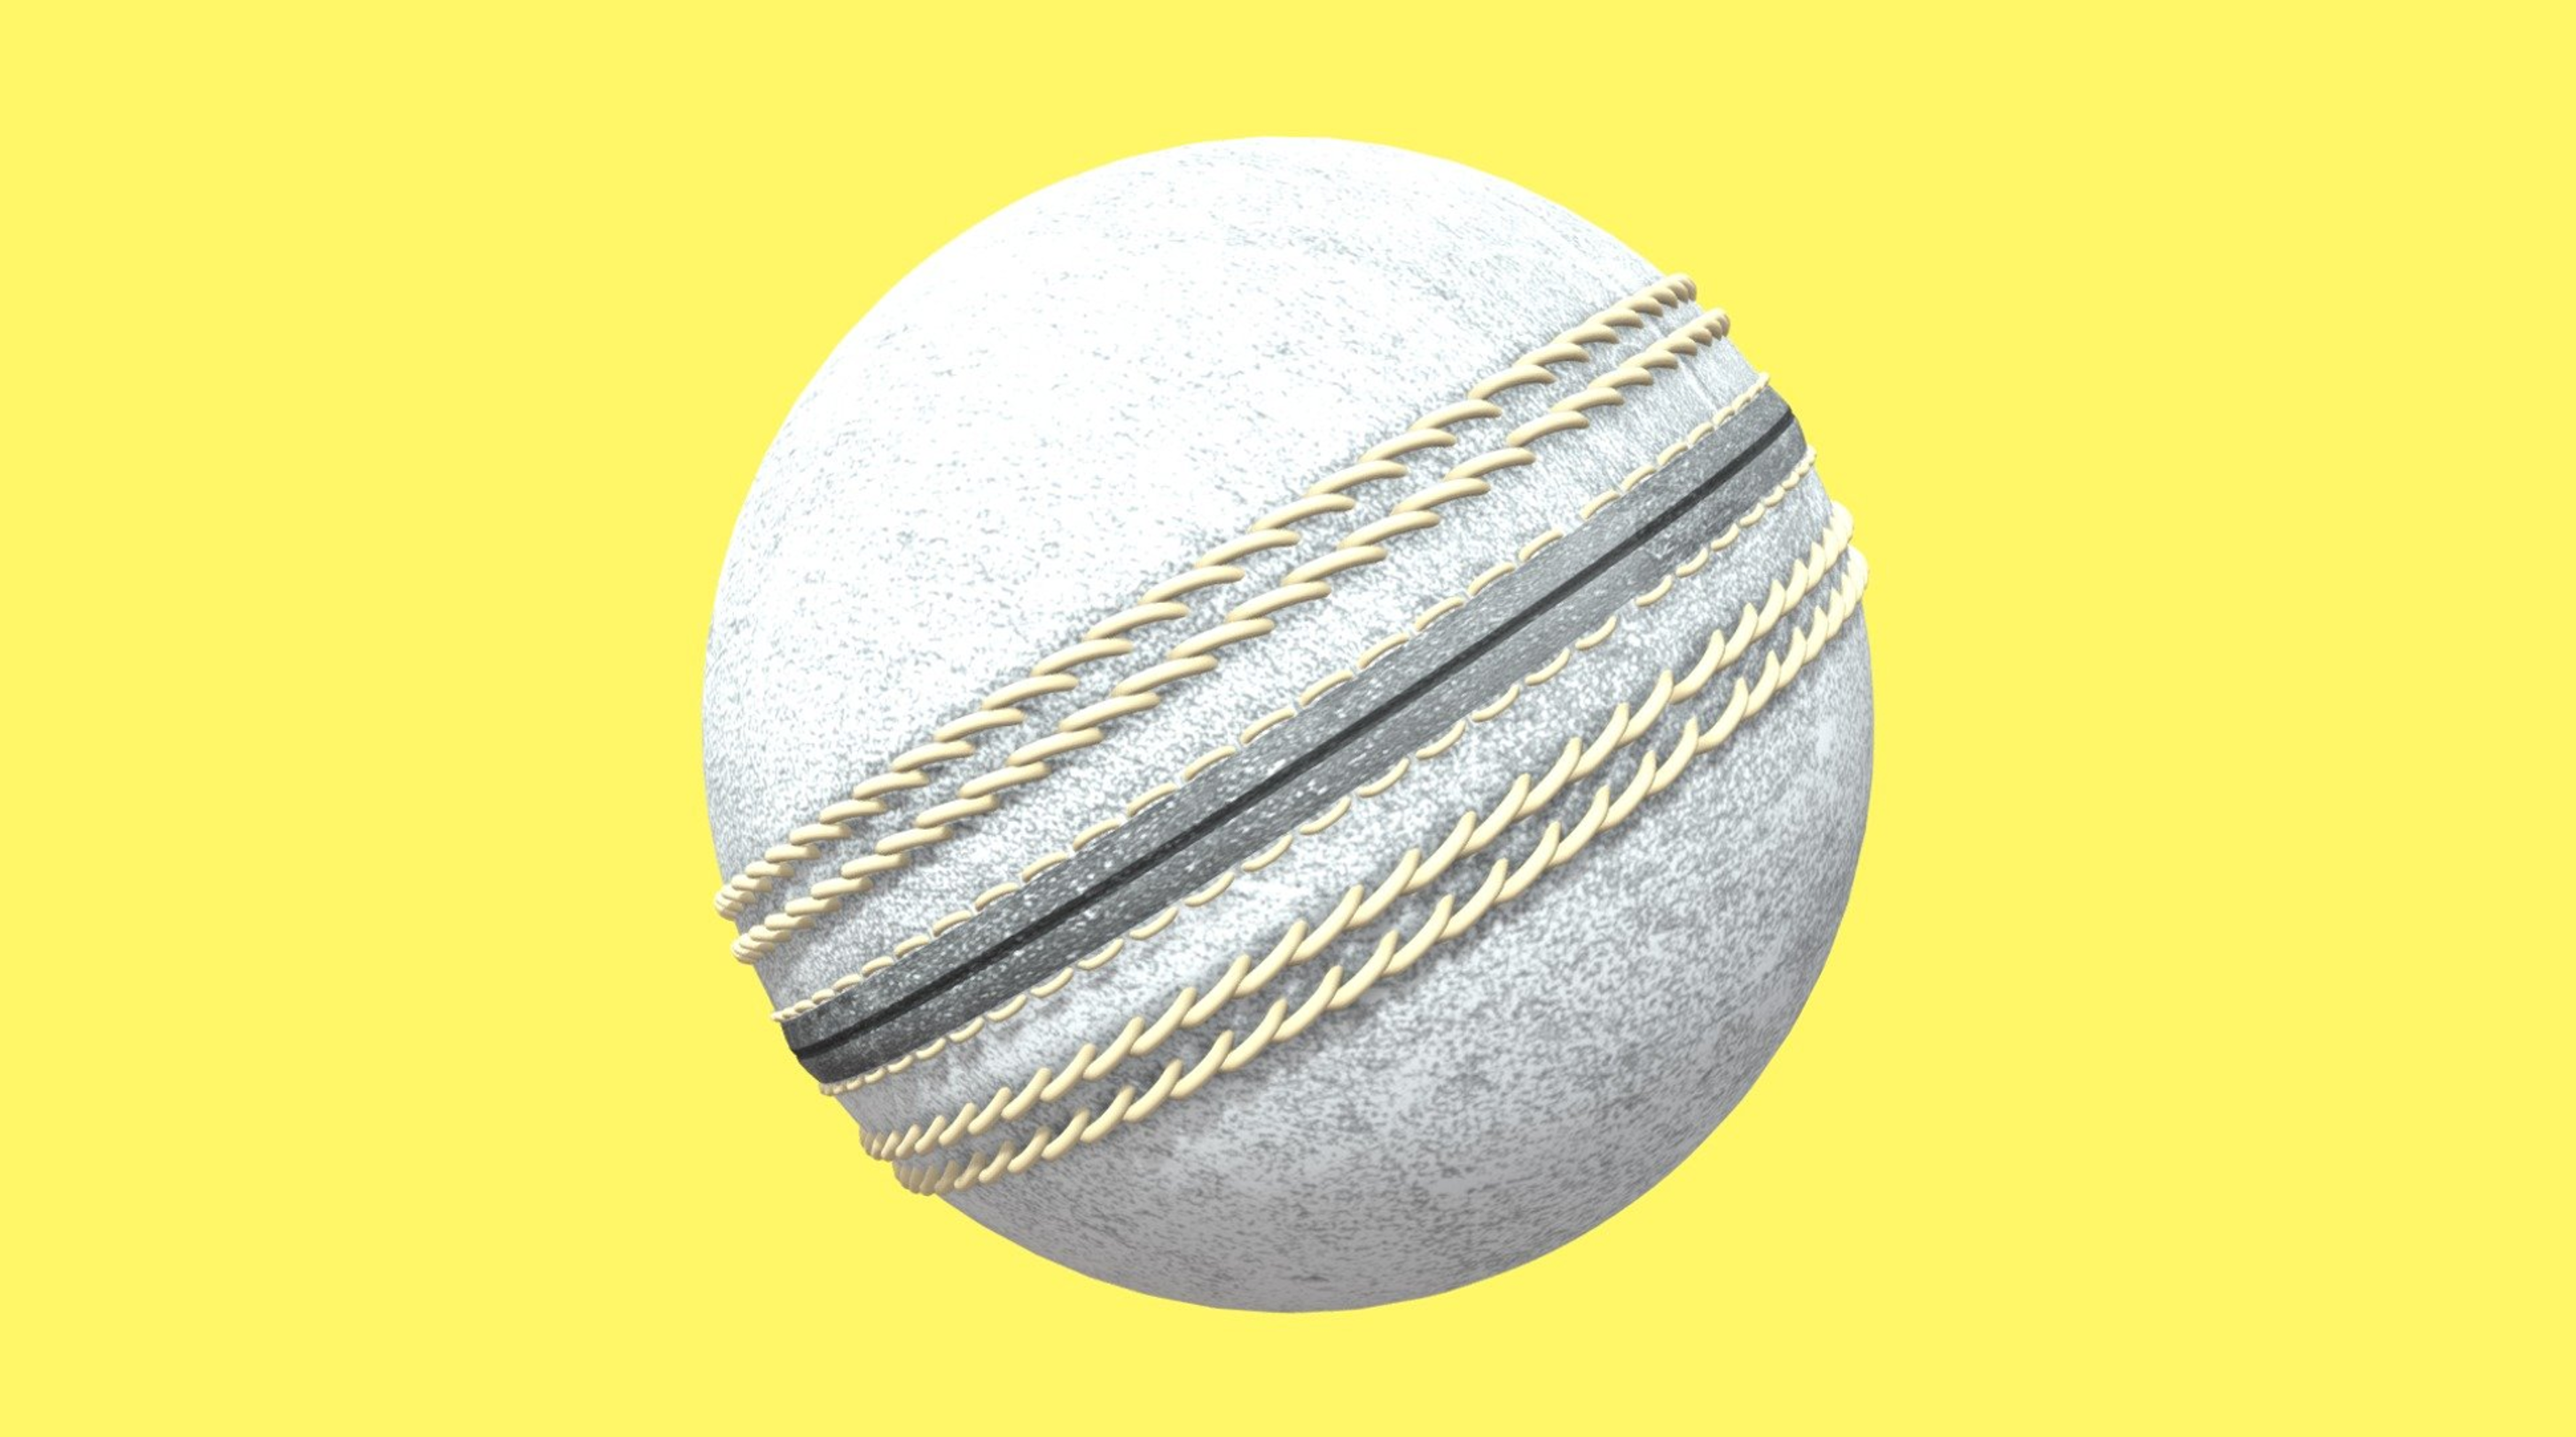
\includegraphics[width=100.5pt,height=57.25pt]{C6M06 - DT - Q1ii.png}};
\draw (410,66.16) node  {\includegraphics[width=87pt,height=57.25pt]{C6M06 - DT - Q1i.png}};
\draw (195,114) node [anchor=north west][inner sep=0.75pt]   [align=left] {Rs. 120};
\draw (381,110) node [anchor=north west][inner sep=0.75pt]   [align=left] {Rs. 120};
\end{tikzpicture}},
optionA={240},
optionB={120},
optionC={180},
optionD={60},
correctoption={B},
leftmini={0.65},
rightmini={0.25},
}
% end-of-question


%-----------------------------------------------------------
%                        Question [ 49 ]
%-----------------------------------------------------------
% start-of-question
\mcqtextbottomOneFour{
questionnumber={2}, 
questiontext={Identify the colour of the denominator.\\
\tikzset{every picture/.style={line width=0.75pt}} 
\hspace{5cm}
\begin{tikzpicture}[x=0.75pt,y=0.75pt,yscale=-1,xscale=1]
\draw  [color={rgb, 255:red, 208; green, 2; blue, 27 }  ,draw opacity=1 ][fill={rgb, 255:red, 175; green, 219; blue, 126 }  ,fill opacity=1 ] (176,57) -- (203,57) -- (203,84) -- (176,84) -- cycle ;
\draw [color={rgb, 255:red, 208; green, 2; blue, 27 }  ,draw opacity=1 ]   (167,88) -- (214,88) ;
\draw  [color={rgb, 255:red, 208; green, 2; blue, 27 }  ,draw opacity=1 ][fill={rgb, 255:red, 248; green, 240; blue, 140 }  ,fill opacity=1 ] (176,93) -- (203,93) -- (203,120) -- (176,120) -- cycle ;
\draw (184,63) node [anchor=north west][inner sep=0.75pt]   [align=left] {5};
\draw (184,99) node [anchor=north west][inner sep=0.75pt]   [align=left] {4};
\end{tikzpicture} },
optionA={Yellow},
optionB={Green},
optionC={Red},
optionD={Green, Yellow},
questionTag={C6M06 - DT - Q2}, 
correctoption={A},
}
% end-of-question

%-----------------------------------------------------------
%                        Question [ 50 ]
%-----------------------------------------------------------
% start-of-question
\mcqtextbottomOneFour{
questionnumber={3}, 
questiontext={Write the fraction of the raw mango from the given image.\\
\hspace{3cm}
\includegraphics[width=10cm, height = 1.5cm]{C6M06 - DT - Q3.png}},
optionA={  {\large{$\frac{1}{6}$}}},
optionB={ {\large{$\frac{7}{10}$}} },
optionC={ {\large{$\frac{1}{7}$}} },
optionD={ {\large{$\frac{6}{7}$}} },
questionTag={C6M06 – DT – Q3}, 
correctoption={C},
}
% end-of-question

%-----------------------------------------------------------
%                        Question [ 51 ]
%-----------------------------------------------------------
% start-of-question
\mcqtextbottomTwoTwo{
questionnumber={4}, 
questionTag={C6M06 - DT - Q4}, 
questiontext={Find the correct representation of {\large{$\frac{3}{5}$}} in the given number lines.},
optionA={\tikzset{every picture/.style={line width=0.75pt}} 
\begin{tikzpicture}[x=0.75pt,y=0.75pt,yscale=-1,xscale=1]
\draw    (112,72) -- (398,72) (150,63.5) -- (150,80.5)(188,63.5) -- (188,80.5)(226,63.5) -- (226,80.5)(264,63.5) -- (264,80.5)(302,63.5) -- (302,80.5)(340,63.5) -- (340,80.5)(378,63.5) -- (378,80.5) ;
\draw [shift={(400,72)}, rotate = 180] [color={rgb, 255:red, 0; green, 0; blue, 0 }  ][line width=0.75]    (10.93,-4.9) .. controls (6.95,-2.3) and (3.31,-0.67) .. (0,0) .. controls (3.31,0.67) and (6.95,2.3) .. (10.93,4.9)   ;
\draw [shift={(110,72)}, rotate = 0] [color={rgb, 255:red, 0; green, 0; blue, 0 }  ][line width=0.75]    (10.93,-4.9) .. controls (6.95,-2.3) and (3.31,-0.67) .. (0,0) .. controls (3.31,0.67) and (6.95,2.3) .. (10.93,4.9)   ;
\draw (180,84) node [anchor=north west][inner sep=0.75pt]   [align=left] {{\large{$\frac{3}{5}$}}};
\draw (373,84) node [anchor=north west][inner sep=0.75pt]   [align=left] {1};
\draw (145.24,84) node [anchor=north west][inner sep=0.75pt]   [align=left] {0};
\end{tikzpicture} },
optionB={\tikzset{every picture/.style={line width=0.75pt}} 
\begin{tikzpicture}[x=0.75pt,y=0.75pt,yscale=-1,xscale=1]
\draw    (112,72) -- (398,72) (150,63.5) -- (150,80.5)(188,63.5) -- (188,80.5)(226,63.5) -- (226,80.5)(264,63.5) -- (264,80.5)(302,63.5) -- (302,80.5)(340,63.5) -- (340,80.5)(378,63.5) -- (378,80.5) ;
\draw [shift={(400,72)}, rotate = 180] [color={rgb, 255:red, 0; green, 0; blue, 0 }  ][line width=0.75]    (10.93,-4.9) .. controls (6.95,-2.3) and (3.31,-0.67) .. (0,0) .. controls (3.31,0.67) and (6.95,2.3) .. (10.93,4.9)   ;
\draw [shift={(110,72)}, rotate = 0] [color={rgb, 255:red, 0; green, 0; blue, 0 }  ][line width=0.75]    (10.93,-4.9) .. controls (6.95,-2.3) and (3.31,-0.67) .. (0,0) .. controls (3.31,0.67) and (6.95,2.3) .. (10.93,4.9)   ;
\draw (335,84) node [anchor=north west][inner sep=0.75pt]   [align=left] {{\large{$\frac{3}{5}$}}};
\draw (145.24,84) node [anchor=north west][inner sep=0.75pt]   [align=left] {0};
\draw (373,84) node [anchor=north west][inner sep=0.75pt]   [align=left] {1};
\end{tikzpicture}},
optionC={\tikzset{every picture/.style={line width=0.75pt}} 
\begin{tikzpicture}[x=0.75pt,y=0.75pt,yscale=-1,xscale=1]
\draw    (112,72) -- (398,72) (150,63.5) -- (150,80.5)(188,63.5) -- (188,80.5)(226,63.5) -- (226,80.5)(264,63.5) -- (264,80.5)(302,63.5) -- (302,80.5)(340,63.5) -- (340,80.5)(378,63.5) -- (378,80.5) ;
\draw [shift={(400,72)}, rotate = 180] [color={rgb, 255:red, 0; green, 0; blue, 0 }  ][line width=0.75]    (10.93,-4.9) .. controls (6.95,-2.3) and (3.31,-0.67) .. (0,0) .. controls (3.31,0.67) and (6.95,2.3) .. (10.93,4.9)   ;
\draw [shift={(110,72)}, rotate = 0] [color={rgb, 255:red, 0; green, 0; blue, 0 }  ][line width=0.75]    (10.93,-4.9) .. controls (6.95,-2.3) and (3.31,-0.67) .. (0,0) .. controls (3.31,0.67) and (6.95,2.3) .. (10.93,4.9)   ;
\draw (218,84) node [anchor=north west][inner sep=0.75pt]   [align=left] {{\large{$\frac{3}{5}$}}};
\draw (180,84) node [anchor=north west][inner sep=0.75pt]   [align=left] {0};
\draw (373,84) node [anchor=north west][inner sep=0.75pt]   [align=left] {1};
\end{tikzpicture}},
optionD={
\tikzset{every picture/.style={line width=0.75pt}} 
\begin{tikzpicture}[x=0.75pt,y=0.75pt,yscale=-1,xscale=1]
\draw    (112,72) -- (398,72) (150,63.5) -- (150,80.5)(188,63.5) -- (188,80.5)(226,63.5) -- (226,80.5)(264,63.5) -- (264,80.5)(302,63.5) -- (302,80.5)(340,63.5) -- (340,80.5)(378,63.5) -- (378,80.5) ;
\draw [shift={(400,72)}, rotate = 180] [color={rgb, 255:red, 0; green, 0; blue, 0 }  ][line width=0.75]    (10.93,-4.9) .. controls (6.95,-2.3) and (3.31,-0.67) .. (0,0) .. controls (3.31,0.67) and (6.95,2.3) .. (10.93,4.9)   ;
\draw [shift={(110,72)}, rotate = 0] [color={rgb, 255:red, 0; green, 0; blue, 0 }  ][line width=0.75]    (10.93,-4.9) .. controls (6.95,-2.3) and (3.31,-0.67) .. (0,0) .. controls (3.31,0.67) and (6.95,2.3) .. (10.93,4.9)   ;
\draw (258,84) node [anchor=north west][inner sep=0.75pt]   [align=left] {{\large{$\frac{3}{5}$}}};
\draw (145.24,84) node [anchor=north west][inner sep=0.75pt]   [align=left] {0};
\draw (333,84) node [anchor=north west][inner sep=0.75pt]   [align=left] {1};
\end{tikzpicture} },
correctoption={D},
}
% end-of-question

%-----------------------------------------------------------
%                        Question [ 52 ]
%-----------------------------------------------------------
% start-of-question
\mcqimgleftFourOne{
questionnumber={5}, 
questionTag={C6M06 – DT – Q5}, 
questiontext={Match the following.},
imgtabletikz = { 
\begin{table}[H]
\centering
\renewcommand{\arraystretch}{1.5}
\begin{tabular}{|p{0.5cm}|p{4cm}|p{0.2cm}|p{0.5cm}|p{2cm}|}
\cline{1-5} 
\multicolumn{2}{|c|}{\textbf{Types of fraction }} & \multirow{5}{*}{} &   
\multicolumn{2}{c|}{\textbf{Examples}} \\
\cline{1-2}\cline{4-5} i.  & Proper fraction
&   & a. & {\large{$\frac{4}{2}$}} \\
\cline{1-2}\cline{4-5} ii. & Improper fraction
&   & b. &  3{\large{$\frac{1}{2}$}}\\
\cline{1-2}\cline{4-5} iii.  & Mixed fraction
&   & c. & {\large{$\frac{3}{4}$}} \\
\hline
\end{tabular}
\end{table}},
optionA={i - a, ii - c, iii - b},
optionB={i - c, ii - a, iii - b},
optionC={i - a, ii - b, iii - c},
optionD={i - b, ii - a, iii - c},
correctoption={B},
leftmini={0.6},
rightmini={0.8},}
% end-of-question


%-----------------------------------------------------------
%                        Question [ 53 ]
%-----------------------------------------------------------
% start-of-question
\mcqtextbottomOneFour{
questionnumber={6}, 
questionTag={C6M06 - DT - Q6}, 
questiontext={Rita wants to find the simplest form {\large{$\frac{25}{175}$}}. Help Rita to find it.},
optionA={ {\large{$\frac{1}{5}$}} },
optionB={ {\large{$\frac{5}{35}$}} },
optionC={ {\large{$\frac{1}{7}$}} },
optionD={ {\large{$\frac{2}{1}$}} },
correctoption={C},
}
% end-of-question
%-----------------------------------------------------------
%                        Question [ 54 ]
%-----------------------------------------------------------
% start-of-question
\mcqtextbottomOneFour{
questionnumber={7}, 
questionTag={C6M06 - DT - Q7}, 
questiontext={ {\large{$\frac{3}{4}$}}, {\large{$\frac{1}{2}$}}  are \rule{40pt}{0.5pt} fractions.},
optionA={Unlike fractions},
optionB={Like fractions},
optionC={Equivalent fractions},
optionD={Mixed fractions},
correctoption={A},
}
% end-of-question
%-----------------------------------------------------------
%                        Question [ 55 ]
%-----------------------------------------------------------
% start-of-question
\mcqtextbottomOneFour{
questionnumber={8}, 
questionTag={C6M06 - DT - Q8}, 
questiontext={Identify the equivalent fraction of  {\large{$\frac{3}{6}$}}.},
optionA={ {\large{$\frac{2}{4}$}} },
optionB={ {\large{$\frac{5}{15}$}} },
optionC={ {\large{$\frac{2}{100}$}} },
optionD={ {\large{$\frac{1}{5}$}} },
correctoption={A},
}
% end-of-question
%-----------------------------------------------------------
%                        Question [ 56 ]
%-----------------------------------------------------------
% start-of-question

\mcqimgleftFourOne{
questionnumber={9}, 
questiontext={Compare the fractions of the remaining pizza slices.},
imgtabletikz = { 
\tikzset{every picture/.style={line width=0.75pt}} 
\begin{tikzpicture}[x=0.75pt,y=0.75pt,yscale=-1,xscale=1]
\draw (221.5,75.5) node  {\includegraphics[width=75.75pt,height=75.75pt]{C6M06 - DT - Q9ii.png}};
\draw   (306,62) -- (339,62) -- (339,95) -- (306,95) -- cycle ;
\draw (419.5,75.5) node  {\includegraphics[width=85pt,height=73pt]{C6M06 - DT - Q9i.png}};
\end{tikzpicture}
},
optionA={$>$},
optionB={$=$},
optionC={$<$},
optionD={Undefined},
questionTag={C6M06 – DT – Q9}, 
leftmini={0.5},
rightmini={0.4}, 
correctoption={C},
}
% end-of-question

%-----------------------------------------------------------
%                        Question [ 57 ]
%-----------------------------------------------------------
% start-of-question
\mcqtextbottomOneFour{
questionnumber={10}, 
questionTag={C6M06 - DT - Q10}, 
questiontext={Add:  {\large{$\frac{2}{15}$}} + {\large{$\frac{1}{5}$}}.},
optionA={ {\large{$\frac{3}{20}$}} },
optionB={ {\large{$\frac{5}{15}$}} },
optionC={ {\large{$\frac{1}{5}$}} },
optionD={ {\large{$\frac{21}{5}$}} },
correctoption={B},
}
% end-of-question
%-----------------------------------------------------------
%                        Question [ 58 ]
%-----------------------------------------------------------

% start-of-question
\mcqtextsideFourOne{
questionnumber={11}, 
questionTag={C6M06 - DT - Q11}, 
questiontext={\\ \medskip
Shalu said {\large{$\frac{2}{5}$}} $-$ {\large{$\frac{1}{5}$}}  is {\large{$\frac{1}{5}$}} \\ \smallskip
Ramu said {\large{$\frac{5}{4}$}} $-$ {\large{$\frac{1}{2}$}} is {\large{$\frac{3}{4}$}} \\ \smallskip
Find whose statement is correct.},
optionA={Shalu’s statement},
optionB={Ramu's statement},
optionC={Both statements are true},
optionD={None of the above},
correctoption={C},
leftmini = {0.5},
rightmini = {0.4},
}
% end-of-question

%-----------------------------------------------------------
%                        Question [  ]
%-----------------------------------------------------------
% start-of-question
\mcqtextbottomOneFour{
questionnumber={12}, 
questiontext={Find the fraction of the blue fish from the given image.\\
\hspace{3cm}
\includegraphics[width=15cm, height = 1.5cm]{C6M06 - DT - Q12.png}},
optionA={  {\large{$\frac{9}{2}$}}},
optionB={ {\large{$\frac{2}{7}$}} },
optionC={ {\large{$\frac{1}{9}$}} },
optionD={ {\large{$\frac{2}{9}$}} },
questionTag={C6M06 – DT – Q12}, 
correctoption={D},
}
% end-of-question

%-----------------------------------------------------------
%                        Question [  ]
%-----------------------------------------------------------
% start-of-question
\mcqtextbottomOneFour{
questionnumber={13}, 
questionTag={C6M06 - DT - Q13}, 
questiontext={Add:  {\large{$\frac{7}{20}$}} + {\large{$\frac{2}{5}$}}.},
optionA={ {\large{$\frac{9}{25}$}} },
optionB={ {\large{$\frac{9}{20}$}} },
optionC={ {\large{$\frac{15}{20}$}} },
optionD={ {\large{$\frac{3}{5}$}} },
correctoption={C},
}
% end-of-question

%-----------------------------------------------------------
%                        Question [ 51 ]
%-----------------------------------------------------------
% start-of-question
\mcqtextbottomTwoTwo{
questionnumber={4}, 
questionTag={C6M06 - DT - Q14}, 
questiontext={Find the correct representation of {\large{$\frac{5}{6}$}} in the given number lines.},
optionA={\tikzset{every picture/.style={line width=0.75pt}} 
\begin{tikzpicture}[x=0.75pt,y=0.75pt,yscale=-1,xscale=1]
\draw    (112,72) -- (398,72) (150,63.5) -- (150,80.5)(188,63.5) -- (188,80.5)(226,63.5) -- (226,80.5)(264,63.5) -- (264,80.5)(302,63.5) -- (302,80.5)(340,63.5) -- (340,80.5)(378,63.5) -- (378,80.5) ;
\draw [shift={(400,72)}, rotate = 180] [color={rgb, 255:red, 0; green, 0; blue, 0 }  ][line width=0.75]    (10.93,-4.9) .. controls (6.95,-2.3) and (3.31,-0.67) .. (0,0) .. controls (3.31,0.67) and (6.95,2.3) .. (10.93,4.9)   ;
\draw [shift={(110,72)}, rotate = 0] [color={rgb, 255:red, 0; green, 0; blue, 0 }  ][line width=0.75]    (10.93,-4.9) .. controls (6.95,-2.3) and (3.31,-0.67) .. (0,0) .. controls (3.31,0.67) and (6.95,2.3) .. (10.93,4.9)   ;
\draw (180,84) node [anchor=north west][inner sep=0.75pt]   [align=left] {{\large{$\frac{5}{6}$}}};
\draw (373,84) node [anchor=north west][inner sep=0.75pt]   [align=left] {1};
\draw (145.24,84) node [anchor=north west][inner sep=0.75pt]   [align=left] {0};
\end{tikzpicture} },
optionB={\tikzset{every picture/.style={line width=0.75pt}} 
\begin{tikzpicture}[x=0.75pt,y=0.75pt,yscale=-1,xscale=1]
\draw    (112,72) -- (398,72) (150,63.5) -- (150,80.5)(188,63.5) -- (188,80.5)(226,63.5) -- (226,80.5)(264,63.5) -- (264,80.5)(302,63.5) -- (302,80.5)(340,63.5) -- (340,80.5)(378,63.5) -- (378,80.5) ;
\draw [shift={(400,72)}, rotate = 180] [color={rgb, 255:red, 0; green, 0; blue, 0 }  ][line width=0.75]    (10.93,-4.9) .. controls (6.95,-2.3) and (3.31,-0.67) .. (0,0) .. controls (3.31,0.67) and (6.95,2.3) .. (10.93,4.9)   ;
\draw [shift={(110,72)}, rotate = 0] [color={rgb, 255:red, 0; green, 0; blue, 0 }  ][line width=0.75]    (10.93,-4.9) .. controls (6.95,-2.3) and (3.31,-0.67) .. (0,0) .. controls (3.31,0.67) and (6.95,2.3) .. (10.93,4.9)   ;
\draw (335,84) node [anchor=north west][inner sep=0.75pt]   [align=left] {{\large{$\frac{5}{6}$}}};
\draw (145.24,84) node [anchor=north west][inner sep=0.75pt]   [align=left] {0};
\draw (373,84) node [anchor=north west][inner sep=0.75pt]   [align=left] {1};
\end{tikzpicture}},
optionC={\tikzset{every picture/.style={line width=0.75pt}} 
\begin{tikzpicture}[x=0.75pt,y=0.75pt,yscale=-1,xscale=1]
\draw    (112,72) -- (398,72) (150,63.5) -- (150,80.5)(188,63.5) -- (188,80.5)(226,63.5) -- (226,80.5)(264,63.5) -- (264,80.5)(302,63.5) -- (302,80.5)(340,63.5) -- (340,80.5)(378,63.5) -- (378,80.5) ;
\draw [shift={(400,72)}, rotate = 180] [color={rgb, 255:red, 0; green, 0; blue, 0 }  ][line width=0.75]    (10.93,-4.9) .. controls (6.95,-2.3) and (3.31,-0.67) .. (0,0) .. controls (3.31,0.67) and (6.95,2.3) .. (10.93,4.9)   ;
\draw [shift={(110,72)}, rotate = 0] [color={rgb, 255:red, 0; green, 0; blue, 0 }  ][line width=0.75]    (10.93,-4.9) .. controls (6.95,-2.3) and (3.31,-0.67) .. (0,0) .. controls (3.31,0.67) and (6.95,2.3) .. (10.93,4.9)   ;
\draw (295,84) node [anchor=north west][inner sep=0.75pt]   [align=left] {{\large{$\frac{5}{6}$}}};
\draw (180,84) node [anchor=north west][inner sep=0.75pt]   [align=left] {0};
\draw (373,84) node [anchor=north west][inner sep=0.75pt]   [align=left] {1};
\end{tikzpicture}},
optionD={
\tikzset{every picture/.style={line width=0.75pt}} 
\begin{tikzpicture}[x=0.75pt,y=0.75pt,yscale=-1,xscale=1]
\draw    (112,72) -- (398,72) (150,63.5) -- (150,80.5)(188,63.5) -- (188,80.5)(226,63.5) -- (226,80.5)(264,63.5) -- (264,80.5)(302,63.5) -- (302,80.5)(340,63.5) -- (340,80.5)(378,63.5) -- (378,80.5) ;
\draw [shift={(400,72)}, rotate = 180] [color={rgb, 255:red, 0; green, 0; blue, 0 }  ][line width=0.75]    (10.93,-4.9) .. controls (6.95,-2.3) and (3.31,-0.67) .. (0,0) .. controls (3.31,0.67) and (6.95,2.3) .. (10.93,4.9)   ;
\draw [shift={(110,72)}, rotate = 0] [color={rgb, 255:red, 0; green, 0; blue, 0 }  ][line width=0.75]    (10.93,-4.9) .. controls (6.95,-2.3) and (3.31,-0.67) .. (0,0) .. controls (3.31,0.67) and (6.95,2.3) .. (10.93,4.9)   ;
\draw (258,84) node [anchor=north west][inner sep=0.75pt]   [align=left] {{\large{$\frac{5}{6}$}}};
\draw (145.24,84) node [anchor=north west][inner sep=0.75pt]   [align=left] {0};
\draw (333,84) node [anchor=north west][inner sep=0.75pt]   [align=left] {1};
\end{tikzpicture} },
correctoption={B},
}
% end-of-question

%-----------------------------------------------------------
%                        Question [ 55 ]
%-----------------------------------------------------------
% start-of-question
\mcqtextbottomOneFour{
questionnumber={15}, 
questionTag={C6M06 - DT - Q15}, 
questiontext={Write the equivalent fraction for {\large{$\frac{10}{15}$}}.},
optionA={ {\large{$\frac{2}{4}$}} },
optionB={ {\large{$\frac{12}{18}$}} },
optionC={ {\large{$\frac{2}{6}$}} },
optionD={ {\large{$\frac{50}{100}$}} },
correctoption={B},
}
% end-of-question

%-----------------------------------------------------------
%                        Question [ 55 ]
%-----------------------------------------------------------
% start-of-question
\mcqtextbottomOneFour{
questionnumber={16}, 
questionTag={C6M06 - DT - Q16}, 
questiontext={Solve: {\large{$\frac{14}{9}$}} $-$ {\large{$\frac{11}{9}$}}},
optionA={ {\large{$\frac{2}{9}$}} },
optionB={ {\large{$\frac{1}{3}$}} },
optionC={ {\large{$\frac{25}{9}$}} },
optionD={ {\large{$\frac{4}{9}$}} },
correctoption={B},
}
% end-of-question

%-----------------------------------------------------------
%                        Question [  ]
%-----------------------------------------------------------
% start-of-question
\mcqtextbottomOneFour{
questionnumber={17}, 
questionTag={C6M06 - DT - Q17}, 
questiontext={ {\large{$\frac{5}{4}$}}, {\large{$\frac{5}{7}$}}  are \rule{40pt}{0.5pt} fractions.},
optionA={Unlike fractions},
optionB={Like fractions},
optionC={Equivalent fractions},
optionD={Mixed fractions},
correctoption={A},
}
% end-of-question



%-----------------------------------------------------------
%                        Question [  ]
%-----------------------------------------------------------
% start-of-question
\mcqtextbottomOneFour{
questionnumber={18}, 
questionTag={C6M06 - DT - Q18}, 
questiontext={ Find the denominator of the fraction. {\large{$\frac{35}{29}$}}.},
optionA={35},
optionB={29},
optionC={35 and 29},
optionD={None of these},
correctoption={B},
}
% end-of-question

%-----------------------------------------------------------
%                        Question [  ]
%-----------------------------------------------------------
% start-of-question
\mcqtextbottomOneFour{
questionnumber={19}, 
questionTag={C6M06 - DT - Q19}, 
questiontext={ Find the fraction of the apple from the given fruits.\\
\hspace{3cm}
\includegraphics[height=1.75cm, width=12cm]{C6M06 - DT - Q19.png}
},
optionA={$\frac{5}{2}$},
optionB={$\frac{2}{5}$},
optionC={$\frac{1}{7}$},
optionD={$\frac{5}{7}$},
correctoption={D},
}
% end-of-question

%-----------------------------------------------------------
%                        Question [  ]
%-----------------------------------------------------------
% start-of-question
\mcqtextbottomOneFour{
questionnumber={20}, 
questionTag={C6M06 - DT - Q20}, 
questiontext={ Compare: $\frac{3}{8}$ \boxed{\color{white}AA} $\frac{4}{12}$},
optionA={$>$},
optionB={=},
optionC={$<$},
optionD={Undefined},
correctoption={A},
}
% end-of-question

%-----------------------------------------------------------
%                        Question [ 59 ]
%-----------------------------------------------------------
% start-of-question
\mcqtextbottomOneFour{
questionnumber={1}, 
questionTag={C6M07 - DT - Q1}, 
questiontext={Complete the table using the place value chart of decimals.\\ \medskip
\hspace{2cm}
\renewcommand{\arraystretch}{1.25}
\begin{tabular}{|>{\centering\arraybackslash}p{2cm}|>{\centering\arraybackslash}p{2cm}|>{\centering\arraybackslash}p{2cm}|>{\centering\arraybackslash}p{3cm}|>{\centering\arraybackslash}p{3cm}|}
\hline
  Tens & Ones & $\boldsymbol{\cdot}$& \rule{80pt}{0.5pt} & Hundredth \\
  \hline
\end{tabular} },
optionA={Tens},
optionB={Oneth},
optionC={Thousandth},
optionD={Tenth},
correctoption={D},
}
% end-of-question

%-----------------------------------------------------------
%                        Question [ 60 ]
%-----------------------------------------------------------
% start-of-question
\mcqimgleftFourOne{
questionnumber={2}, 
questionTag={C6M07 - DT - Q2}, 
questiontext={ To elevate the child in the seesaw above, how much weight should be placed on his opposite side?},
imgtabletikz = { 
\includegraphics[width=9cm, height=3cm]{C6M07 - DT - Q2.png}   },
optionA={20.25 kg},
optionB={20.05 kg},
optionC={20.75 kg},
optionD={20.100 kg},
correctoption={C},
leftmini={0.6},
rightmini={0.8},
}
% end-of-question


%-----------------------------------------------------------
%                        Question [ 61 ]
%-----------------------------------------------------------
% start-of-question
\mcqtextbottomOneFour{
questionnumber={3}, 
questionTag={C6M07 - DT - Q3}, 
questiontext={Convert the following numbers.\\ \smallskip
\qquad i. 1.2 into fraction. \qquad ii. {\large{$\frac{1}{10}$}} into decimals.},
optionA={i. {\large{$\frac{12}{10}$}}, ii. 1.0},
optionB={i. {\large{$\frac{12}{10}$}}, ii. 0.1},
optionC={i. {\large{$\frac{1.2}{10}$}}, ii. 1.0},
optionD={i. {\large{$\frac{2}{10}$}}, ii. 0.1},
correctoption={B},
}
% end-of-question

%-----------------------------------------------------------
%                        Question [62 ]
%-----------------------------------------------------------
% start-of-question
\mcqimgleftFourOne{
questionnumber={4}, 
questionTag={C6M07 - DT - Q4},
questiontext={Find the height of the man in cm.},
imgtabletikz  = { 
\tikzset{every picture/.style={line width=0.75pt}} 
\begin{tikzpicture}[x=0.75pt,y=0.75pt,yscale=-1,xscale=1]
\draw    (158.17,20.61) -- (158.71,122.62) ;
\draw [shift={(158.73,125.62)}, rotate = 269.69] [fill={rgb, 255:red, 0; green, 0; blue, 0 }  ][line width=0.08]  [draw opacity=0] (8.93,-4.29) -- (0,0) -- (8.93,4.29) -- cycle    ;
\draw [shift={(158.15,17.61)}, rotate = 89.69] [fill={rgb, 255:red, 0; green, 0; blue, 0 }  ][line width=0.08]  [draw opacity=0] (8.93,-4.29) -- (0,0) -- (8.93,4.29) -- cycle    ;
\draw (129.64,73.42) node  {\includegraphics[width=27.96pt,height=87.57pt]{C6M07 - DT - Q4.png}};
\draw (159.49,62.28) node [anchor=north west][inner sep=0.75pt]   [align=left] {\textbf{1.5 m}};
\end{tikzpicture} },
optionA={1.5 cm},
optionB={15 cm},
optionC={150 cm},
optionD={5100 cm},
correctoption={C},
leftmini={0.65},
rightmini={0.35},
}
% end-of-question

%-----------------------------------------------------------
%                        Question [ 63 ]
%-----------------------------------------------------------
% start-of-question
\mcqtextbottomOneFour{
questionnumber={5}, 
questionTag={C6M07 - DT - Q5}, 
questiontext={Add: $0.1 + 2.55$},
optionA={2.551},
optionB={3.55},
optionC={2.56},
optionD={2.65},
correctoption={D},
}
% end-of-question

%-----------------------------------------------------------
%                        Question [ 64]
%-----------------------------------------------------------
% start-of-question
\mcqtextbottomOneFour{
questionnumber={6}, 
questionTag={C6M07 - DT - Q6}, 
questiontext={Vidya got 4.5 liters of milk and she gave 3.5 liters to her neighbor. How many liters of milk does she have now? },
optionA={8 liters},
optionB={7.5 liters},
optionC={3.5 liters},
optionD={1 liter},
correctoption={D},
}
% end-of-question

%-----------------------------------------------------------
%                        Question [ ]
%-----------------------------------------------------------
% start-of-question
\mcqtextbottomOneFour{
questionnumber={7}, 
questionTag={C6M07 - DT - Q7}, 
questiontext={Represent the following in decimals.\\
\hspace{3cm}70 rupees and 50 paise},
optionA={\rupee 7.050},
optionB={\rupee 70.5},
optionC={\rupee 7050},
optionD={\rupee 70.05},
correctoption={B},
}
% end-of-question

%-----------------------------------------------------------
%                        Question [ ]
%-----------------------------------------------------------
% start-of-question
\mcqtextbottomOneFour{
questionnumber={8}, 
questionTag={C6M07 - DT - Q8}, 
questiontext={Aasha paid \rupee 105.75 for the history guide and \rupee 85.8 for the Tamil guide. Find Aasha's entire spending.},
optionA={\rupee 114.33},
optionB={\rupee 19.95},
optionC={\rupee 190.83},
optionD={\rupee 191.55},
correctoption={D},
}
% end-of-question

%-----------------------------------------------------------
%                        Question [ ]
%-----------------------------------------------------------
% start-of-question
\mcqtextbottomOneFour{
questionnumber={9}, 
questionTag={C6M07 - DT - Q9}, 
questiontext={Subtract 34.007 from 67.07},
optionA={33.077},
optionB={33},
optionC={33.063},
optionD={101.077},
correctoption={C},
}
% end-of-question

%-----------------------------------------------------------
%                        Question [ ]
%-----------------------------------------------------------
% start-of-question
\mcqtextbottomOneFour{
questionnumber={10}, 
questionTag={C6M07 - DT - Q10}, 
questiontext={If a book weighs 12500 g, what is the weight of that book in kilograms?},
optionA={12500000 kg},
optionB={0.0125 kg},
optionC={12.5 kg},
optionD={125 kg},
correctoption={C},
}
% end-of-question

%-----------------------------------------------------------
%                        Question [ 64]
%-----------------------------------------------------------
% start-of-question
\mcqtextbottomOneFour{
questionnumber={11}, 
questionTag={C6M07 - DT - Q11}, 
questiontext={Ponni bought 5.5 kg of sweets and gave 3.4 kg to her friend Reena. Find the remaining kg of sweets with Ponni.},
optionA={8.9 kg},
optionB={2.1 kg},
optionC={1 kg},
optionD={1.2 kg},
correctoption={B},
}
% end-of-question

%-----------------------------------------------------------
%                        Question [ 61 ]
%-----------------------------------------------------------
% start-of-question
\mcqtextbottomOneFour{
questionnumber={12}, 
questionTag={C6M07 - DT - Q12}, 
questiontext={Convert 0.95 into a fraction.},
optionA={ {\large{$\frac{0}{95}$}} },
optionB={ {\large{$\frac{0.95}{100}$}} },
optionC={ {\large{$\frac{95}{100}$}} },
optionD={ {\large{$\frac{9.5}{100}$}} },
correctoption={C},
}
% end-of-question

%-----------------------------------------------------------
%                        Question [ 61 ]
%-----------------------------------------------------------
% start-of-question
\mcqtextbottomOneFour{
questionnumber={13}, 
questionTag={C6M07 - DT - Q13}, 
questiontext={Convert {\large{$\frac{25}{10}$}} into decimals.},
optionA={25.0  },
optionB={0.25 },
optionC={ 2.5},
optionD={ 25.10},
correctoption={C},
}
% end-of-question

%-----------------------------------------------------------
%                        Question [  ]
%-----------------------------------------------------------
% start-of-question
\mcqtextbottomOneFour{
questionnumber={14}, 
questionTag={C6M07 - DT - Q14}, 
questiontext={Add: 22.22 + 3.33},
optionA={2.555 },
optionB={25.55},
optionC={ 55.52},
optionD={555.2},
correctoption={B},
}
% end-of-question

%-----------------------------------------------------------
%                        Question [ ]
%-----------------------------------------------------------
% start-of-question
\mcqimgleftFourOne{
questionnumber={15}, 
questionTag={C6M07 - DT - Q15}, 
questiontext={Subtract.},
imgtabletikz  = {
\begin{table}[H]
\centering
\begin{tabular}{cccccc}
& 1 & 2 &. & 4 &  \\
$-$ &  & 1 & .&1&6\\
\hline
& & &&& \\
\hline
\end{tabular}
\end{table} },
optionA={0.08},
optionB={13.56},
optionC={ 11.24},
optionD={11.36},
correctoption={C},
leftmini={0.5},
rightmini={0.4},
}

% end-of-question

%-----------------------------------------------------------
%                        Question [ 65]
%-----------------------------------------------------------
% start-of-question
\mcqtextbottomOneFour{
questionnumber={1}, 
questionTag={C6M10 - DT - Q1}, 
questiontext={Write {\large{$\frac{1}{10}$}} in the form of ratio. },
optionA={ 1 : 1},
optionB={10 : 1},
optionC={1 : 10},
optionD={1 : 1, 10 : 10},
correctoption={C},
}
% end-of-question


%-----------------------------------------------------------
%                        Question [ 66]
%-----------------------------------------------------------
% start-of-question
\mcqtextbottomOneFour{
questionnumber={2}, 
questionTag={C6M10 - DT - Q2}, 
questiontext={Find the ratio of 2 kg to 800 g. },
optionA={ 1 : 400},
optionB={2 : 800},
optionC={5 : 2},
optionD={2 : 8},
correctoption={C},
}
% end-of-question

%-----------------------------------------------------------
%                        Question [ 67]
%-----------------------------------------------------------
% start-of-question
\mcqtextbottomOneFour{
questionnumber={3}, 
questionTag={C6M10 - DT - Q3}, 
questiontext={Pick the shape that contains the ratio in the simplest form.\\
\tikzset{every picture/.style={line width=0.75pt}} 
\begin{tikzpicture}[x=0.75pt,y=0.75pt,yscale=-1,xscale=1]
\draw   (68,73) -- (186,73) -- (186,110.6) -- (68,110.6) -- cycle ;
\draw   (236,91.3) .. controls (236,78.43) and (260.62,68) .. (291,68) .. controls (321.38,68) and (346,78.43) .. (346,91.3) .. controls (346,104.17) and (321.38,114.6) .. (291,114.6) .. controls (260.62,114.6) and (236,104.17) .. (236,91.3) -- cycle ;
\draw   (441.5,64) -- (502,111.6) -- (381,111.6) -- cycle ;
\draw   (547,56) -- (617,56) -- (617,118.6) -- (547,118.6) -- cycle ;
\draw (105,84) node [anchor=north west][inner sep=0.75pt]   [align=left] {20 : 20};
\draw (270,84) node [anchor=north west][inner sep=0.75pt]   [align=left] {6 : 27};
\draw (421,84) node [anchor=north west][inner sep=0.75pt]   [align=left] {3 : 10};
\draw (558,84) node [anchor=north west][inner sep=0.75pt]   [align=left] {10 : 5};
\end{tikzpicture}
},
optionA={ Rectangle},
optionB={Oval},
optionC={Triangle},
optionD={Square},
correctoption={C},
}
% end-of-question

%-----------------------------------------------------------
%                        Question [ 68]
%----------------------------------------------------------
% start-of-question
\mcqtextbottomOneFour{
questionnumber={4}, 
questionTag={C6M10 - DT - Q4}, 
questiontext={Find the correct pair based on the equivalent ratio.},
optionA={ 10 : 5 and 20 : 15},
optionB={ 3 : 6 and 6 : 12 },
optionC={1 : 5 and 7 : 11},
optionD={ 3 : 7 and 3 : 8 },
correctoption={B},
}
% end-of-question

%-----------------------------------------------------------
%                        Question [ 69]
%----------------------------------------------------------
% start-of-question
\mcqtextbottomOneFour{
questionnumber={5}, 
questionTag={C6M10 - DT - Q5}, 
questiontext={Find the value of $x$ in the following proportion.\quad 10 : 8 : : $x$ : 24},
optionA={ 30},
optionB={ 35 },
optionC={100},
optionD={ 50},
correctoption={A},
}
% end-of-question

%-----------------------------------------------------------
%                        Question [ 70]
%----------------------------------------------------------
% start-of-question
\mcqtextbottomOneFour{
questionnumber={6}, 
questionTag={C6M10 - DT - Q6}, 
questiontext={If one milkshake costs Rs. 35, how many milkshakes can you buy for Rs. 140?},
optionA={ 4},
optionB={ 8 },
optionC={5},
optionD={ 10},
correctoption={A},
}
% end-of-question

%-----------------------------------------------------------
%                        Question [ 71]
%----------------------------------------------------------
% start-of-question
\mcqtextbottomOneFour{
questionnumber={7}, 
questionTag={C6M10 - DT - Q7}, 
questiontext={Anu and Abi ate chocolates in the ratio 4 : 9. If Abi ate 36 chocolates, find the number of chocolates eaten by Anu.},
optionA={ 16 chocolates},
optionB={ 81 chocolates },
optionC={ 72 chocolates},
optionD={ 56 chocolates},
correctoption={A},
}
% end-of-question

%-----------------------------------------------------------
%                        Question []
%-----------------------------------------------------------
% start-of-question
\mcqtextbottomOneFour{
questionnumber={8}, 
questionTag={C6M10 - DT - Q8},
questiontext={The height of Seema is 134 cm and the height of Rheema is 155 cm. Find the ratio of the height of the Rheema to the height of the Seema.},
optionA={134 : 155},
optionB={134 + 155},
optionC={67 : 77},
optionD={155 : 134},
correctoption={D},}
% end-of-question

%-----------------------------------------------------------
%                        Question []
%-----------------------------------------------------------
% start-of-question
\mcqtextbottomOneFour{
questionnumber={9}, 
questionTag={C6M10 - DT - Q9},
questiontext={If one quantity in the ratio is 8 g, the unit of the other quantity should be in \rule{80pt}{0.5pt}, to compare them. },
optionA={gram},
optionB={kilogram},
optionC={liter},
optionD={Either a and b},
correctoption={A},
}
% end-of-question

%-----------------------------------------------------------
%                        Question []
%-----------------------------------------------------------
% start-of-question
\mcqtextbottomOneFour{
questionnumber={10}, 
questionTag={C6M10 - DT - Q10}, 
questiontext={Represent the given ratio in the form of a fraction. \quad 10 : 19 },
optionA={ {\large{$\frac{19}{10}$}}},
optionB={{\large{$\frac{9}{1}$}}},
optionC={{\large{$\frac{10}{19}$}}},
optionD={10{\large{$\frac{1}{19}$}}},
correctoption={C},
}
% end-of-question

%-----------------------------------------------------------
%                        Question []
%-----------------------------------------------------------
% start-of-question
\mcqtextbottomOneFour{
questionnumber={11}, 
questionTag={C6M10 - DT - Q11},
questiontext={Find the ratio of 5 m to 700 cm.},
optionA={ 500 : 7},
optionB={5 : 700},
optionC={ 5 : 7},
optionD={ 0.05 : 700},
correctoption={C},}
% end-of-question

%-----------------------------------------------------------
%                        Question []
%-----------------------------------------------------------
% start-of-question
\mcqtextbottomOneFour{
questionnumber={12}, 
questionTag={C6M10 - DT - Q12},
questiontext={Find the equivalent ratio of 1 : 7},
optionA={7 : 1},
optionB={7 : 14 },
optionC={8 : 56},
optionD={100 : 70 },
correctoption={C},}
% end-of-question

%-----------------------------------------------------------
%                        Question []
%-----------------------------------------------------------
% start-of-question
\mcqtextbottomOneFour{
questionnumber={13}, 
questionTag={C6M10 - DT - Q13},
questiontext={Find the value of $y$ in the given proportion.\\
\hspace{4cm} 5 : 7 : : 20 : $y$},
optionA={35},
optionB={28},
optionC={100},
optionD={32},
correctoption={B},}
% end-of-question

%-----------------------------------------------------------
%                        Question []
%-----------------------------------------------------------
% start-of-question
\mcqtextbottomOneFour{
questionnumber={14}, 
questionTag={C6M10 - DT - Q14},
questiontext={ If one \includegraphics[height=1cm,width=1cm]{C6M10 - DT - Q14.png}    costs Rs. 10. What is the total cost of the following roses?\\
\hspace{3cm} \includegraphics[height=1cm,width=1cm]{C6M10 - DT - Q14.png} \includegraphics[height=1cm,width=1cm]{C6M10 - DT - Q14.png} \includegraphics[height=1cm,width=1cm]{C6M10 - DT - Q14.png} \includegraphics[height=1cm,width=1cm]{C6M10 - DT - Q14.png} \includegraphics[height=1cm,width=1cm]{C6M10 - DT - Q14.png}  },
optionA={Rs. 5},
optionB={Rs. 25},
optionC={Rs. 50},
optionD={Rs. 100},
correctoption={C},
}
% end-of-question

%-----------------------------------------------------------
%                        Question []
%-----------------------------------------------------------
% start-of-question
\mcqtextbottomOneFour{
questionnumber={15}, 
questionTag={C6M10 - DT - Q15},
questiontext={Rathu and Rithi collected coins in the ratio of 8 : 5. If Rithi collected 40 coins, find the number of coins collected by Rathu.},
optionA={25 coins},
optionB={ 64 coins},
optionC={ 13 coins},
optionD={ 53 coins},
correctoption={B},}
% end-of-question

%-----------------------------------------------------------
%                        Question []
%-----------------------------------------------------------
% start-of-question
\mcqtextbottomOneFour{
questionnumber={16}, 
questionTag={C6M10 - DT - Q16},
questiontext={To compare two quantities, if one quantity in the ratio is represented in meter, the unit of the other quantity should be in \rule{40pt}{0.5pt}.},
optionA={meter},
optionB={centimeter},
optionC={Either a or b},
optionD={gram},
correctoption={A},}
% end-of-question

%-----------------------------------------------------------
%                        Question []
%-----------------------------------------------------------
% start-of-question
\mcqtextbottomOneFour{
questionnumber={17}, 
questionTag={C6M10 - DT - Q17},
questiontext={If  four milkshake costs Rs. 140, how many milkshakes can you buy for Rs. 245?},
optionA={385},
optionB={105},
optionC={35},
optionD={7},
correctoption={D},}
% end-of-question

%-----------------------------------------------------------
%                        Question [ 72]
%----------------------------------------------------------
% start-of-question
\mcqtextbottomOneFour{
questionnumber={1}, 
questionTag={C6M09 - DT - Q1}, 
questiontext={How many variables are present in the expression $5x + 4y - 3z+2x-y$?},
optionA={ 5},
optionB={ 3},
optionC={ 2},
optionD={ 4},
correctoption={B},
}
% end-of-question

%-----------------------------------------------------------
%                        Question [ 73]
%----------------------------------------------------------
% start-of-question
\mcqimgleftFourOne{
questionnumber={2}, 
questionTag={C6M09 - DT - Q2}, 
questiontext={How many line segments are required to make $n$ number of the given shape?},
imgtabletikz  = {\tikzset{every picture/.style={line width=0.75pt}} 
\begin{tikzpicture}[x=0.75pt,y=0.75pt,yscale=-1,xscale=1]
\draw  [line width=1.5]  (149,189.73) -- (178.32,92) -- (286.68,92) -- (316,189.73) -- cycle ;
\end{tikzpicture}},
optionA={$n$},
optionB={4},
optionC={4$n$},
optionD={$ n \times n $},
correctoption={C},
leftmini={0.4},
rightmini={0.5},
}
% end-of-question


%-----------------------------------------------------------
%                        Question [74  ]
%-----------------------------------------------------------

% start-of-question
\mcqimgleftFourOne{
questionnumber={3}, 
questionTag={C6M09 - DT - Q3},
questiontext={Match the following.},
imgtabletikz  = { \begin{table}[H]
\centering
\renewcommand{\arraystretch}{1.25}
\begin{tabular}{|p{0.4cm}|p{5cm}|p{0.2cm}|p{0.4cm}|p{2cm}|}
\cline{1-5} 
\multicolumn{2}{|c|}{\textbf{Statement }} & 
\multirow{5}{*}{} &   
\multicolumn{2}{c|}{\textbf{Expression}} \\
\cline{1-2}\cline{4-5} i.  & 10 times of $y$ is added to 5
&   & a. & $-$10$y$ \\
\cline{1-2}\cline{4-5} ii. & 10 less than a number is 5
&   & b. &  10$y$$+$5\\
\cline{1-2}\cline{4-5} iii.  & 10 is multiplied by $-$$y$
&   & c. & $y$$-$10 = 5 \\
\hline
\end{tabular}
\end{table}},
optionA={i - c, ii - b, iii - a},
optionB={i - a, ii - b, iii - c},
optionC={i - a, ii - c, iii - b},
optionD={i - b, ii - c, iii - a},
correctoption={D},
leftmini={0.6},
rightmini={0.3},
}
% end-of-question

%-----------------------------------------------------------
%                        Question [75  ]
%-----------------------------------------------------------
% start-of-question
\mcqtextbottomOneFour{
questionnumber={4}, 
questionTag={C6M09 - DT - Q4},
questiontext={The cost of a bat is Rs. 8$x$, the cost of a ball is Rs. 5$x$ and the total cost of the ball and bat is Rs. 13$x$. Frame an equation for the given statement.},
optionA={$5x$ $+$ $13x$ = 8$x$},
optionB={$8x$ $+$ $5x$ = $13x$},
optionC={$8x$ = $5x$},
optionD={$8x$ $-$  $5x$ = $13x$},
correctoption={B},}
% end-of-question

%-----------------------------------------------------------
%                        Question [76]
%-----------------------------------------------------------
% start-of-question
\mcqtextbottomOneFour{
questionnumber={5}, 
questionTag={C6M09 - DT - Q5},
questiontext={The number of blue balls is 125 less than the number of green balls. If the total number of balls is 275,  find the number of green balls.},
optionA={75},
optionB={400},
optionC={200},
optionD={175},
correctoption={C},}
% end-of-question

%-----------------------------------------------------------
%                        Question []
%-----------------------------------------------------------
% start-of-question
\mcqtextbottomOneFour{
questionnumber={6}, 
questionTag={C6M09 - DT - Q6},
questiontext={Find the expression that has only one variable and only one constant in it.},
optionA={$xy+1$},
optionB={$c+v+1$},
optionC={$u-3$},
optionD={$1g$},
correctoption={C},}
% end-of-question

%-----------------------------------------------------------
%                        Question []
%-----------------------------------------------------------
% start-of-question
\mcqtextbottomOneFour{
questionnumber={7}, 
questionTag={C6M09 - DT - Q7},
questiontext={An equation does not contain \rule{80pt}{0.5pt} sign.},
optionA={$+$},
optionB={$-$},
optionC={$=$},
optionD={$>$},
correctoption={D},}
% end-of-question

%-----------------------------------------------------------
%                        Question []
%-----------------------------------------------------------
% start-of-question
\mcqtextbottomOneFour{
questionnumber={8}, 
questionTag={C6M09 - DT - Q8},
questiontext={Choose an expression that consists of only one variable.},
optionA={$x+y+1$},
optionB={$1x+1y$},
optionC={$x+5x$},
optionD={$1$},
correctoption={C},}
% end-of-question

%-----------------------------------------------------------
%                        Question []
%-----------------------------------------------------------
% start-of-question
\mcqtextbottomOneFour{
questionnumber={9}, 
questionTag={C6M09 - DT - Q9},
questiontext={Product of 3, and $a$ is added to 10 times of $x$ is \rule{80pt}{0.5pt}.},
optionA={$3 + a \times 10 + x$},
optionB={$3 + a +10x$},
optionC={$3+a+10+x$},
optionD={$3a+10 \times x$},
correctoption={D},}
% end-of-question


%-----------------------------------------------------------
%                        Question [ 77]
%-----------------------------------------------------------
% start-of-question
\mcqimgleftFourOne{
questionnumber={1}, 
questionTag={C6M16 - DT - Q1},
questiontext={Identify the color of the perimeter and area regions in the given square.},
imgtabletikz = { \includegraphics[width=3cm, height=3cm]{C6M16 - DT - Q1.png}},
optionA={Perimeter - Brown, Area - Grey},
optionB={Perimeter - Grey, Area - Blue},
optionC={Perimeter - Brown, Area - Blue},
optionD={Perimeter - White, Area - Red},
correctoption={C},
leftmini={0.4},
rightmini={0.5},
}
% end-of-question

%-----------------------------------------------------------
%                        Question [78  ]
%-----------------------------------------------------------

% start-of-question
\mcqimgleftFourOne{
questionnumber={2}, 
questionTag={C6M16 - DT - Q2},
questiontext={Match the following. (Hint: a = side length)},
imgtabletikz  = { \begin{table}[H]
\centering
\renewcommand{\arraystretch}{1.25}
\begin{tabular}{|p{0.5cm}|p{4cm}|p{0.2cm}|p{0.5cm}|p{1.5cm}|}
\cline{1-5} 
\multicolumn{2}{|c|}{\textbf{Shape }} & 
\multirow{5}{*}{} &   
\multicolumn{2}{c|}{\textbf{Perimeter}} \\
\cline{1-2}\cline{4-5} i.  & Square
&   & a. &5$a$ \\
\cline{1-2}\cline{4-5} ii. & Regular pentagon
&   & b. &  3$a$\\
\cline{1-2}\cline{4-5} iii.  & Equilateral triangle
&   & c. & 4$a$ \\
\hline
\end{tabular}
\end{table}},
optionA={i - c, ii - b, iii – a},
optionB={i - c, ii - a, iii - b},
optionC={i - a, ii - b, iii - c},
optionD={i - b, ii - a, iii - c},
correctoption={B},
leftmini={0.5},
rightmini={0.4},
}
% end-of-question


%-----------------------------------------------------------
%                        Question [79  ]
%-----------------------------------------------------------
% start-of-question
\mcqimgleftFourOne{
questionnumber={3}, 
questionTag={C6M16 – DT – Q3},
questiontext={Which shape has the greater perimeter? },
imgtabletikz  = {\tikzset{every picture/.style={line width=0.75pt}} 
\begin{tikzpicture}[x=0.75pt,y=0.75pt,yscale=-1,xscale=1]

\draw  [line width=1.5]  (411.17,95.11) -- (467.28,94.37) -- (467.5,139.94) -- (544.53,138.93) -- (544.75,183.98) -- (411.62,185.72) -- cycle ;
\draw  [line width=1.5]  (285,98) -- (350,98) -- (220,211.92) -- (220,154.96) -- cycle ;
\draw (488.4,96.05) node [anchor=north west][inner sep=0.75pt]  [rotate=-88.86] [align=left] {1 m};
\draw (415,80) node [anchor=north west][inner sep=0.75pt]   [align=left] {1 m};
\draw (372.89,135.39) node [anchor=north west][inner sep=0.75pt]   [align=left] {2 m};
\draw (550.11,155.91) node [anchor=north west][inner sep=0.75pt]   [align=left] {1 m};
\draw (497.62,120.34) node [anchor=north west][inner sep=0.75pt]   [align=left] {2 m};
\draw (460,190) node [anchor=north west][inner sep=0.75pt]   [align=left] {3 m};
\draw (453,213) node [anchor=north west][inner sep=0.75pt]   [align=left] {\textbf{Shape B}};
\draw (178,175) node [anchor=north west][inner sep=0.75pt]   [align=left] {1 m};
\draw (222,108) node [anchor=north west][inner sep=0.75pt]   [align=left] {2 m};
\draw (300,80) node [anchor=north west][inner sep=0.75pt]   [align=left] {1.5 m};
\draw (287,157.96) node [anchor=north west][inner sep=0.75pt]   [align=left] {4 m};
\draw (252,213) node [anchor=north west][inner sep=0.75pt]   [align=left] {\textbf{Shape A}};
\end{tikzpicture}},
optionA={Shape A},
optionB={Shape B},
optionC={Both are equal},
optionD={Perimeter cannot be calculated},
correctoption={B},
leftmini={0.55},
rightmini={0.35},}
% end-of-question

%-----------------------------------------------------------
%                        Question [ 80]
%-----------------------------------------------------------
% start-of-question
\mcqimgleftFourOne{
questionnumber={4}, 
questionTag={C6M16 - DT - Q4}, 
questiontext={Find the area of the given rectangular notebook.},
imgtabletikz  = {
\tikzset{every picture/.style={line width=0.75pt}} 
\begin{tikzpicture}[x=0.75pt,y=0.75pt,yscale=-1,xscale=1]
\draw (244.25,113.49) node  {\includegraphics[width=81.38pt,height=95.24pt]{C6M16 - DT - Q4.png}};
\draw [line width=1.5]    (303.41,66.12) -- (302.75,165.15) ;
\draw [shift={(302.73,169.15)}, rotate = 270.38] [fill={rgb, 255:red, 0; green, 0; blue, 0 }  ][line width=0.08]  [draw opacity=0] (11.61,-5.58) -- (0,0) -- (11.61,5.58) -- cycle    ;
\draw [shift={(303.43,62.12)}, rotate = 90.38] [fill={rgb, 255:red, 0; green, 0; blue, 0 }  ][line width=0.08]  [draw opacity=0] (11.61,-5.58) -- (0,0) -- (11.61,5.58) -- cycle    ;
\draw [line width=1.5]    (288.16,183.81) -- (208.8,183.17) ;
\draw [shift={(204.8,183.14)}, rotate = 0.46] [fill={rgb, 255:red, 0; green, 0; blue, 0 }  ][line width=0.08]  [draw opacity=0] (11.61,-5.58) -- (0,0) -- (11.61,5.58) -- cycle    ;
\draw [shift={(292.16,183.84)}, rotate = 180.46] [fill={rgb, 255:red, 0; green, 0; blue, 0 }  ][line width=0.08]  [draw opacity=0] (11.61,-5.58) -- (0,0) -- (11.61,5.58) -- cycle    ;
\draw (307.65,109.71) node [anchor=north west][inner sep=0.75pt]   [align=left] {45 cm};
\draw (224.51,190.15) node [anchor=north west][inner sep=0.75pt]   [align=left] {31 cm};
\end{tikzpicture} },
optionA={ $1395$ cm},
optionB={$2025$ cm},
optionC={$1395$ sq. cm},
optionD={$2025$ sq. cm},
correctoption={C},
leftmini={0.5},
rightmini={0.4},
}
% end-of-question


%-----------------------------------------------------------
%                        Question [ 81]
%-----------------------------------------------------------
% start-of-question
\mcqtextbottomOneFour{
questionnumber={5}, 
questionTag={C6M16 - DT - Q5}, 
questiontext={Find the area of a square whose side is 65 m.},
optionA={ $65$ sq. cm},
optionB={$3925$ sq. m},
optionC={$6925$ sq. m},
optionD={$4225$ sq. m},
correctoption={D},
}
% end-of-question

%-----------------------------------------------------------
%                        Question [ 82 ]
%-----------------------------------------------------------
% start-of-question
\mcqimgleftFourOne{
questionnumber={6}, 
questionTag={C6M16 - DT - Q6},
questiontext={Find the area of the given shape.},
imgtabletikz  = {

\tikzset{every picture/.style={line width=0.75pt}} 
\begin{tikzpicture}[x=0.75pt,y=0.75pt,yscale=-1,xscale=1]
\draw   (119.74,86.74) -- (161.22,86.41) -- (161.49,120.1) -- (280.98,119.14) -- (281.25,152.44) -- (120.27,153.74) -- cycle ;
\draw (200,98) node [anchor=north west][inner sep=0.75pt]   [align=left] {3 cm};
\draw (285,128) node [anchor=north west][inner sep=0.75pt]   [align=left] {1 cm};
\draw (77,118) node [anchor=north west][inner sep=0.75pt]   [align=left] {2 cm};
\draw (119,65) node [anchor=north west][inner sep=0.75pt]   [align=left] {1 cm};
\draw (182.38,80.74) node [anchor=north west][inner sep=0.75pt]  [rotate=-88.86] [align=left] {1 cm};
\end{tikzpicture}},
optionA={17 sq. cm},
optionB={8 sq. cm},
optionC={5 sq. cm},
optionD={4 sq. m},
correctoption={C},
leftmini={0.5},
rightmini={0.4},
}
% end-of-question

%-----------------------------------------------------------
%                        Question [ ]
%-----------------------------------------------------------
% start-of-question
\mcqimgleftFourOne{
questionnumber={7}, 
questionTag={C6M16 - DT - Q7}, 
questiontext={Find the area of the given shape.(Hint: Area of one square = 1 sq. units)},
imgtabletikz = { 
\tikzset{every picture/.style={line width=0.75pt}} 
\begin{tikzpicture}[x=0.75pt,y=0.75pt,yscale=-1,xscale=1] 
\draw  [draw opacity=0] (128,62) -- (313,62) -- (313,220) -- (128,220) -- cycle ; \draw   (128,62) -- (128,220)(154,62) -- (154,220)(180,62) -- (180,220)(206,62) -- (206,220)(232,62) -- (232,220)(258,62) -- (258,220)(284,62) -- (284,220)(310,62) -- (310,220) ; \draw   (128,62) -- (313,62)(128,88) -- (313,88)(128,114) -- (313,114)(128,140) -- (313,140)(128,166) -- (313,166)(128,192) -- (313,192)(128,218) -- (313,218) ; \draw    ;
%Straight Lines [id:da14655635186522487] 
\draw [color={rgb, 255:red, 208; green, 2; blue, 27 }  ,draw opacity=1 ][line width=2.25]    (154,114) -- (154,192) ;
%Straight Lines [id:da14322094621586046] 
\draw [color={rgb, 255:red, 208; green, 2; blue, 27 }  ,draw opacity=1 ][line width=2.25]    (154,114) -- (258,114) ;
%Straight Lines [id:da04388106338841058] 
\draw [color={rgb, 255:red, 208; green, 2; blue, 27 }  ,draw opacity=1 ][line width=2.25]    (258,114) -- (258,166) ;
%Straight Lines [id:da9427134835938675] 
\draw [color={rgb, 255:red, 208; green, 2; blue, 27 }  ,draw opacity=1 ][line width=2.25]    (258,166) -- (284,166) ;
%Straight Lines [id:da9459120073758434] 
\draw [color={rgb, 255:red, 208; green, 2; blue, 27 }  ,draw opacity=1 ][line width=2.25]    (154,192) -- (284,192) ;
%Straight Lines [id:da6348039665906768] 
\draw [color={rgb, 255:red, 208; green, 2; blue, 27 }  ,draw opacity=1 ][line width=2.25]    (284,166) -- (284,192) ;
\end{tikzpicture}
},
optionA={12 sq.units},
optionB={13 sq.units},
optionC={8 sq.units},
optionD={18 sq.units},
correctoption={B},
leftmini={0.5},
rightmini={0.4},}
% end-of-question

%-----------------------------------------------------------
%                        Question [ ]
%-----------------------------------------------------------
% start-of-question
\mcqtextbottomOneFour{
questionnumber={8}, 
questionTag={C6M16 - DT - Q8}, 
questiontext={Find the side length of the equilateral triangle if its perimeter is 15 cm.},
optionA={ 3 cm},
optionB={5 cm},
optionC={5 sq. cm},
optionD={15 cm},
correctoption={B},
}
% end-of-question

%-----------------------------------------------------------
%                        Question [ ]
%-----------------------------------------------------------
% start-of-question
\mcqimgleftFourOne{
questionnumber={9}, 
questionTag={C6M16 - DT - Q9},
questiontext={Ramu walks around the lake in the evening. The path he walked is to be considered as the \rule{80pt}{0.5pt}},
imgtabletikz = { \includegraphics[width=3cm, height=3.5cm]{C6M16 - DT - Q9.png}},
optionA={Area},
optionB={Perimeter},
optionC={Volume},
optionD={Both a and b},
correctoption={B},
leftmini={0.4},
rightmini={0.5},
}
% end-of-question
%-----------------------------------------------------------
%                        Question [ ]
%-----------------------------------------------------------
% start-of-question
\mcqtextbottomOneFour{
questionnumber={10}, 
questionTag={C6M16 - DT - Q10}, 
questiontext={Find the shape that has a perimeter as 5a.},
optionA={Square},
optionB={Pentagon},
optionC={Hexagon},
optionD={Rectangle},
correctoption={B},
}
% end-of-question

%-----------------------------------------------------------
%                        Question [ ]
%-----------------------------------------------------------
% start-of-question
\mcqimgleftFourOne{
questionnumber={11}, 
questionTag={C6M16 - DT - Q11},
questiontext={Which shape has the greatest perimeter?},
imgtabletikz = {
\tikzset{every picture/.style={line width=0.75pt}} 
\begin{tikzpicture}[x=0.75pt,y=0.75pt,yscale=-1,xscale=1]
\draw   (120,209.02) -- (143.1,132.02) -- (213.9,132.02) -- (237,209.02) -- cycle ;
\draw   (321.5,172.83) -- (354.32,140.02) -- (422.57,140.02) -- (455.39,172.83) -- (455.39,209.02) -- (455.39,209.02) -- (321.5,209.02) -- (321.5,209.02) -- cycle ;
\draw (159,213) node [anchor=north west][inner sep=0.75pt]   [align=left] {3 cm};
\draw (374,211) node [anchor=north west][inner sep=0.75pt]   [align=left] {4 cm};
\draw (165,111) node [anchor=north west][inner sep=0.75pt]   [align=left] {2 cm};
\draw (374,122) node [anchor=north west][inner sep=0.75pt]   [align=left] {2 cm};
\draw (98.24,179.48) node [anchor=north west][inner sep=0.75pt]  [rotate=-290.7] [align=left] {4.5 cm};
\draw (240.73,142.54) node [anchor=north west][inner sep=0.75pt]  [rotate=-72.94] [align=left] {4.5 cm};
\draw (304.37,157.96) node [anchor=north west][inner sep=0.75pt]  [rotate=-317.86] [align=left] {1.2 cm};
\draw (435.67,126.98) node [anchor=north west][inner sep=0.75pt]  [rotate=-44.44] [align=left] {1.2 cm};
\draw (157,240) node [anchor=north west][inner sep=0.75pt]   [align=left] {Shape M};
\draw (360,237) node [anchor=north west][inner sep=0.75pt]   [align=left] {Shape N};
\draw (454.79,184.61) node [anchor=north west][inner sep=0.75pt]  [rotate=-358.52] [align=left] {1 cm};
\draw (285.79,182.61) node [anchor=north west][inner sep=0.75pt]  [rotate=-358.52] [align=left] {1 cm};
\end{tikzpicture} },
optionA={Shape M},
optionB={Shape N},
optionC={Both are equal},
optionD={Perimeter cannot be calculated},
correctoption={A},
leftmini={0.4},
rightmini={0.3},
}
% end-of-question

%-----------------------------------------------------------
%                        Question [ ]
%-----------------------------------------------------------
% start-of-question
\mcqtextbottomOneFour{
questionnumber={12}, 
questionTag={C6M16 - DT - Q12}, 
questiontext={If the length of a rectangular garden is 65 m and its breadth is 40 m, find its area. },
optionA={ 105 m},
optionB={2600 cm},
optionC={2600 sq. m},
optionD={105 sq. cm},
correctoption={C},
}
% end-of-question


%-----------------------------------------------------------
%                        Question [ ]
%-----------------------------------------------------------
% start-of-question
\mcqimgleftFourOne{
questionnumber={13}, 
questionTag={C6M16 - DT - Q13},
questiontext={Find the area of the following shape.},
imgtabletikz = {
\tikzset{every picture/.style={line width=0.75pt}}
\begin{tikzpicture}[x=0.75pt,y=0.75pt,yscale=-1,xscale=1]
\draw   (392,173) -- (337,172.84) -- (337.15,123.83) -- (241.99,123.55) -- (242.16,66.87) -- (392.31,67.32) -- cycle ;
\draw (349,178) node [anchor=north west][inner sep=0.75pt]   [align=left] {4 cm};
\draw (273,126) node [anchor=north west][inner sep=0.75pt]   [align=left] {6 cm};
\draw (299,47) node [anchor=north west][inner sep=0.75pt]   [align=left] {10 cm};
\draw (317.84,166.92) node [anchor=north west][inner sep=0.75pt]  [rotate=-270.53] [align=left] {4 cm};
\draw (218.84,113.92) node [anchor=north west][inner sep=0.75pt]  [rotate=-270.53] [align=left] {4 cm};
\draw (393.84,124.92) node [anchor=north west][inner sep=0.75pt]  [rotate=-270.53] [align=left] {8 cm};
\end{tikzpicture}
},
optionA={36 sq. cm},
optionB={96 sq. cm},
optionC={56 sq. cm},
optionD={4 sq. cm},
correctoption={C},
leftmini={0.45},
rightmini={0.45},
}
% end-of-question

%-----------------------------------------------------------
%                        Question [ ]
%-----------------------------------------------------------
% start-of-question
\mcqimgleftFourOne{
questionnumber={14}, 
questionTag={C6M16 - DT - Q14},
questiontext={Find the area of the given shape.(Hint: Area of one square = 1 sq. units)},
imgtabletikz = {
\tikzset{every picture/.style={line width=0.75pt}} 
\begin{tikzpicture}[x=0.75pt,y=0.75pt,yscale=-1,xscale=1]
\draw  [draw opacity=0] (147,81) -- (332,81) -- (332,239) -- (147,239) -- cycle ; \draw   (147,81) -- (147,239)(173,81) -- (173,239)(199,81) -- (199,239)(225,81) -- (225,239)(251,81) -- (251,239)(277,81) -- (277,239)(303,81) -- (303,239)(329,81) -- (329,239) ; \draw   (147,81) -- (332,81)(147,107) -- (332,107)(147,133) -- (332,133)(147,159) -- (332,159)(147,185) -- (332,185)(147,211) -- (332,211)(147,237) -- (332,237) ; \draw    ;
\draw [color={rgb, 255:red, 208; green, 2; blue, 27 }  ,draw opacity=1 ][line width=2.25]    (173,107) -- (173,185) ;
\draw [color={rgb, 255:red, 208; green, 2; blue, 27 }  ,draw opacity=1 ][line width=2.25]    (173,107) -- (277,107) ;
\draw [color={rgb, 255:red, 208; green, 2; blue, 27 }  ,draw opacity=1 ][line width=2.25]    (277,107) -- (277,159) ; 
\draw [color={rgb, 255:red, 208; green, 2; blue, 27 }  ,draw opacity=1 ][line width=2.25]    (277,159) -- (303,159) ;
\draw [color={rgb, 255:red, 208; green, 2; blue, 27 }  ,draw opacity=1 ][line width=2.25]    (173,185) -- (251,185) ;
\draw [color={rgb, 255:red, 208; green, 2; blue, 27 }  ,draw opacity=1 ][line width=2.25]    (303,159) -- (303,211) ;
\draw [color={rgb, 255:red, 208; green, 2; blue, 27 }  ,draw opacity=1 ][line width=2.25]    (251,185) -- (251,211) ; 
\draw [color={rgb, 255:red, 208; green, 2; blue, 27 }  ,draw opacity=1 ][line width=2.25]    (251,211) -- (303,211) ;
\end{tikzpicture}   
},
optionA={15 sq.units},
optionB={18 sq.units},
optionC={8 sq.units},
optionD={16 sq.units},
correctoption={A},
leftmini={0.5},
rightmini={0.4},
}
% end-of-question


%-----------------------------------------------------------
%                        Question [ 81]
%-----------------------------------------------------------
% start-of-question
\mcqtextbottomOneFour{
questionnumber={15}, 
questionTag={C6M16 - DT - Q15}, 
questiontext={If the side of the square is 13 cm, find its area.},
optionA={ $156$ sq. cm},
optionB={$26$ sq. cm},
optionC={$169$ sq. cm},
optionD={$13$ sq. cm},
correctoption={C},
}
% end-of-question
%-----------------------------------------------------------
%                        Question [ 83]
%-----------------------------------------------------------
% start-of-question
\mcqtextbottomOneFour{
questionnumber={1}, 
questionTag={C6M14 - DT - Q1}, 
questiontext={How many lines of symmetry can be drawn in a square? },
optionA={ Two},
optionB={Three},
optionC={Four},
optionD={Infinite},
correctoption={C},
}
% end-of-question

%-----------------------------------------------------------
%                        Question [ 84]
%-----------------------------------------------------------
% start-of-question
\mcqimgleftFourOne{
questionnumber={2}, 
questionTag={C6M14 - DT - Q2}, 
questiontext={Find the number of lines of symmetry for the given image.},
imgtabletikz = { 
\includegraphics[width=4cm, height=3cm]{C6M14 - DT - Q2.png}  },
optionA={Zero},
optionB={Two},
optionC={Three},
optionD={One},
correctoption={D},
leftmini={0.5},
rightmini={0.4},}
% end-of-question

%-----------------------------------------------------------
%                        Question [ 85]
%-----------------------------------------------------------
% start-of-question
\mcqtextbottomOneFour{
questionnumber={3}, 
questionTag={C6M14 - DT - Q3}, 
questiontext={Find the correct reflection of the given image.\\
\medskip
\tikzset{every picture/.style={line width=0.75pt}} 
\hspace{3cm}
\begin{tikzpicture}[x=0.75pt,y=0.75pt,yscale=-1,xscale=1]
\draw (220.5,127.5) node  {\includegraphics[width=119.25pt,height=95.25pt]{C6M14 - DT - Q3.png}};
\draw (256,38) node [anchor=north west][inner sep=0.75pt]   [align=left] {Mirror};
\end{tikzpicture} },
optionA={\includegraphics[width=70pt,height=50pt]{C6M14 - DT - Q3i.png}},
optionB={\includegraphics[width=70pt,height=50pt]{C6M14 - DT - Q3ii.png}},
optionC={\includegraphics[width=70pt,height=50pt]{C6M14 - DT - Q3iii.png}},
optionD={\includegraphics[width=70pt,height=50pt]{C6M14 - DT - Q3iv.png}},
correctoption={D},}
% end-of-question

%-----------------------------------------------------------
%                        Question [ ]
%-----------------------------------------------------------
% start-of-question
\mcqtextbottomOneFour{
questionnumber={4}, 
questionTag={C6M14 - DT - Q4}, 
questiontext={Pick the symmetrical ink blot. },
optionA={\includegraphics[width=70pt,height=50pt]{C6M14 - DT - Q4i.png}},
optionB={\includegraphics[width=70pt,height=50pt]{C6M14 - DT - Q4ii.png}},
optionC={\includegraphics[width=70pt,height=50pt]{C6M14 - DT - Q4iii.png}},
optionD={\includegraphics[width=70pt,height=50pt]{C6M14 - DT - Q4iv.png}},
correctoption={B},}
% end-of-question

%-----------------------------------------------------------
%                        Question [ ]
%-----------------------------------------------------------
% start-of-question
\mcqtextbottomOneFour{
questionnumber={5}, 
questionTag={C6M14 - DT - Q5}, 
questiontext={Select the correct lines of symmetry drawn in the image. \\


\tikzset{every picture/.style={line width=0.75pt}} %set default line width to 0.75pt        
\hspace{4cm}
\begin{tikzpicture}[x=0.75pt,y=0.75pt,yscale=-1,xscale=1]
%uncomment if require: \path (0,300); %set diagram left start at 0, and has height of 300

%Shape: Rectangle [id:dp5790411124552954] 
\draw   (212,65) -- (391,65) -- (391,139) -- (212,139) -- cycle ;
%Straight Lines [id:da5059393145196986] 
\draw    (205.85,61.77) -- (402.15,143.23) ;
\draw [shift={(404,144)}, rotate = 202.54] [color={rgb, 255:red, 0; green, 0; blue, 0 }  ][line width=0.75]    (10.93,-4.9) .. controls (6.95,-2.3) and (3.31,-0.67) .. (0,0) .. controls (3.31,0.67) and (6.95,2.3) .. (10.93,4.9)   ;
\draw [shift={(204,61)}, rotate = 22.54] [color={rgb, 255:red, 0; green, 0; blue, 0 }  ][line width=0.75]    (10.93,-4.9) .. controls (6.95,-2.3) and (3.31,-0.67) .. (0,0) .. controls (3.31,0.67) and (6.95,2.3) .. (10.93,4.9)   ;
%Straight Lines [id:da7397131514242781] 
\draw    (194.84,148.22) -- (404.16,59.78) ;
\draw [shift={(406,59)}, rotate = 157.09] [color={rgb, 255:red, 0; green, 0; blue, 0 }  ][line width=0.75]    (10.93,-4.9) .. controls (6.95,-2.3) and (3.31,-0.67) .. (0,0) .. controls (3.31,0.67) and (6.95,2.3) .. (10.93,4.9)   ;
\draw [shift={(193,149)}, rotate = 337.09] [color={rgb, 255:red, 0; green, 0; blue, 0 }  ][line width=0.75]    (10.93,-4.9) .. controls (6.95,-2.3) and (3.31,-0.67) .. (0,0) .. controls (3.31,0.67) and (6.95,2.3) .. (10.93,4.9)   ;
%Straight Lines [id:da8088779392608945] 
\draw    (195,102) -- (409,102) ;
\draw [shift={(411,102)}, rotate = 180] [color={rgb, 255:red, 0; green, 0; blue, 0 }  ][line width=0.75]    (10.93,-4.9) .. controls (6.95,-2.3) and (3.31,-0.67) .. (0,0) .. controls (3.31,0.67) and (6.95,2.3) .. (10.93,4.9)   ;
\draw [shift={(193,102)}, rotate = 0] [color={rgb, 255:red, 0; green, 0; blue, 0 }  ][line width=0.75]    (10.93,-4.9) .. controls (6.95,-2.3) and (3.31,-0.67) .. (0,0) .. controls (3.31,0.67) and (6.95,2.3) .. (10.93,4.9)   ;


% Text Node
\draw (177,95) node [anchor=north west][inner sep=0.75pt]   [align=left] {x};
% Text Node
\draw (402,124) node [anchor=north west][inner sep=0.75pt]   [align=left] {y};
% Text Node
\draw (400,66) node [anchor=north west][inner sep=0.75pt]   [align=left] {z};


\end{tikzpicture}

},
optionA={only x},
optionB={only y},
optionC={only z},
optionD={All the above},
correctoption={A},}
% end-of-question


%-----------------------------------------------------------
%                        Question [ ]
%-----------------------------------------------------------
% start-of-question
\mcqtextbottomOneFour{
questionnumber={1}, 
questionTag={C6M18 - DT - Q1}, 
questiontext={Find the next number in the following sequence.\\
\qquad \qquad \qquad 26, 39, 52, 65, \rule{40pt}{0.5pt}},
optionA={76},
optionB={78},
optionC={80},
optionD={47},
correctoption={B},
}
% end-of-question

%-----------------------------------------------------------
%                        Question [ ]
%-----------------------------------------------------------
% start-of-question
\mcqtextbottomOneFour{
questionnumber={2}, 
questionTag={C6M18 - DT - Q2}, 
questiontext={How many squares will be there in the next pattern?
\vspace{0.5cm}

\tikzset{every picture/.style={line width=0.75pt}} %set default line width to 0.75pt        

\begin{tikzpicture}[x=0.75pt,y=0.75pt,yscale=-1,xscale=1]
%uncomment if require: \path (0,300); %set diagram left start at 0, and has height of 300

%Shape: Rectangle [id:dp7086628820654319] 
\draw   (81,126) -- (124,126) -- (124,163) -- (81,163) -- cycle ;
%Shape: Rectangle [id:dp5525998421916072] 
\draw   (341,88) -- (384,88) -- (384,125) -- (341,125) -- cycle ;
%Shape: Rectangle [id:dp17911580398515214] 
\draw   (384,88) -- (427,88) -- (427,125) -- (384,125) -- cycle ;
%Shape: Rectangle [id:dp8053633489211967] 
\draw   (341,125) -- (384,125) -- (384,162) -- (341,162) -- cycle ;
%Shape: Rectangle [id:dp543501783548644] 
\draw   (384,125) -- (427,125) -- (427,162) -- (384,162) -- cycle ;

%Shape: Rectangle [id:dp6215515648530843] 
\draw   (427,88) -- (470,88) -- (470,125) -- (427,125) -- cycle ;
%Shape: Rectangle [id:dp24674957386652574] 
\draw   (427,125) -- (470,125) -- (470,162) -- (427,162) -- cycle ;
%Shape: Rectangle [id:dp32852315352418593] 
\draw   (341,162) -- (384,162) -- (384,199) -- (341,199) -- cycle ;
%Shape: Rectangle [id:dp9841807562690805] 
\draw   (384,162) -- (427,162) -- (427,199) -- (384,199) -- cycle ;
%Shape: Rectangle [id:dp22633821801042697] 
\draw   (427,162) -- (470,162) -- (470,199) -- (427,199) -- cycle ;

%Shape: Rectangle [id:dp005649626975611888] 
\draw   (196,105) -- (239,105) -- (239,142) -- (196,142) -- cycle ;
%Shape: Rectangle [id:dp5391571819294534] 
\draw   (239,105) -- (282,105) -- (282,142) -- (239,142) -- cycle ;
%Shape: Rectangle [id:dp8187601989747315] 
\draw   (196,142) -- (239,142) -- (239,179) -- (196,179) -- cycle ;
%Shape: Rectangle [id:dp3736993094037133] 
\draw   (239,142) -- (282,142) -- (282,179) -- (239,179) -- cycle ;





\end{tikzpicture}
},
optionA={4},
optionB={8},
optionC={12},
optionD={16},
correctoption={D},
}
% end-of-question

%-----------------------------------------------------------%                        Question [ ]
%-----------------------------------------------------------
% start-of-question
\mcqtextbottomOneFour{
questionnumber={3}, 
questionTag={C6M18 - DT - Q3}, 
questiontext={Find the seventh shape in the given pattern. \\
\vspace{0.5cm}
\tikzset{every picture/.style={line width=0.75pt}} %set default line width to 0.75pt        

\begin{tikzpicture}[x=0.75pt,y=0.75pt,yscale=-1,xscale=1]
%uncomment if require: \path (0,300); %set diagram left start at 0, and has height of 300

%Shape: Triangle [id:dp22793212967179732] 
\draw   (72.5,90) -- (106,146) -- (39,146) -- cycle ;
%Shape: Ellipse [id:dp8236704284193204] 
\draw  [color={rgb, 255:red, 0; green, 0; blue, 0 }  ,draw opacity=1 ][fill={rgb, 255:red, 0; green, 0; blue, 0 }  ,fill opacity=1 ] (67.5,87) .. controls (67.5,83.96) and (69.74,81.5) .. (72.5,81.5) .. controls (75.26,81.5) and (77.5,83.96) .. (77.5,87) .. controls (77.5,90.04) and (75.26,92.5) .. (72.5,92.5) .. controls (69.74,92.5) and (67.5,90.04) .. (67.5,87) -- cycle ;
%Shape: Ellipse [id:dp5578368186466107] 
\draw  [color={rgb, 255:red, 0; green, 0; blue, 0 }  ,draw opacity=1 ][fill={rgb, 255:red, 0; green, 0; blue, 0 }  ,fill opacity=1 ] (34,146) .. controls (34,142.96) and (36.24,140.5) .. (39,140.5) .. controls (41.76,140.5) and (44,142.96) .. (44,146) .. controls (44,149.04) and (41.76,151.5) .. (39,151.5) .. controls (36.24,151.5) and (34,149.04) .. (34,146) -- cycle ;
%Shape: Ellipse [id:dp6928275736563558] 
\draw  [color={rgb, 255:red, 0; green, 0; blue, 0 }  ,draw opacity=1 ][fill={rgb, 255:red, 0; green, 0; blue, 0 }  ,fill opacity=1 ] (102,146) .. controls (102,142.96) and (104.24,140.5) .. (107,140.5) .. controls (109.76,140.5) and (112,142.96) .. (112,146) .. controls (112,149.04) and (109.76,151.5) .. (107,151.5) .. controls (104.24,151.5) and (102,149.04) .. (102,146) -- cycle ;

%Shape: Rectangle [id:dp09773978111328496] 
\draw   (145,100) -- (190,100) -- (190,139) -- (145,139) -- cycle ;
%Shape: Rectangle [id:dp5109773068388199] 
\draw   (230.17,122.14) -- (261,91) -- (292.17,121.85) -- (261.34,152.99) -- cycle ;
%Shape: Ellipse [id:dp1123068118949686] 
\draw  [color={rgb, 255:red, 0; green, 0; blue, 0 }  ,draw opacity=1 ][fill={rgb, 255:red, 0; green, 0; blue, 0 }  ,fill opacity=1 ] (258,89) .. controls (258,85.96) and (260.24,83.5) .. (263,83.5) .. controls (265.76,83.5) and (268,85.96) .. (268,89) .. controls (268,92.04) and (265.76,94.5) .. (263,94.5) .. controls (260.24,94.5) and (258,92.04) .. (258,89) -- cycle ;
%Shape: Ellipse [id:dp2431987078403015] 
\draw  [color={rgb, 255:red, 0; green, 0; blue, 0 }  ,draw opacity=1 ][fill={rgb, 255:red, 0; green, 0; blue, 0 }  ,fill opacity=1 ] (287.17,119.35) .. controls (287.17,116.31) and (289.4,113.85) .. (292.17,113.85) .. controls (294.93,113.85) and (297.17,116.31) .. (297.17,119.35) .. controls (297.17,122.39) and (294.93,124.85) .. (292.17,124.85) .. controls (289.4,124.85) and (287.17,122.39) .. (287.17,119.35) -- cycle ;
%Shape: Ellipse [id:dp3358293136018293] 
\draw  [color={rgb, 255:red, 0; green, 0; blue, 0 }  ,draw opacity=1 ][fill={rgb, 255:red, 0; green, 0; blue, 0 }  ,fill opacity=1 ] (225.17,122.14) .. controls (225.17,119.1) and (227.41,116.64) .. (230.17,116.64) .. controls (232.94,116.64) and (235.17,119.1) .. (235.17,122.14) .. controls (235.17,125.18) and (232.94,127.64) .. (230.17,127.64) .. controls (227.41,127.64) and (225.17,125.18) .. (225.17,122.14) -- cycle ;
%Shape: Ellipse [id:dp1223871060326085] 
\draw  [color={rgb, 255:red, 0; green, 0; blue, 0 }  ,draw opacity=1 ][fill={rgb, 255:red, 0; green, 0; blue, 0 }  ,fill opacity=1 ] (256.34,152.99) .. controls (256.34,149.95) and (258.58,147.49) .. (261.34,147.49) .. controls (264.1,147.49) and (266.34,149.95) .. (266.34,152.99) .. controls (266.34,156.03) and (264.1,158.49) .. (261.34,158.49) .. controls (258.58,158.49) and (256.34,156.03) .. (256.34,152.99) -- cycle ;
\draw   (332,99) -- (377,99) -- (377,138) -- (332,138) -- cycle ;
\draw   (439.91,95.93) -- (467.38,115.11) -- (457.62,147.17) -- (424.12,147.8) -- (413.17,116.13) -- cycle ;
\draw  [color={rgb, 255:red, 0; green, 0; blue, 0 }  ,draw opacity=1 ][fill={rgb, 255:red, 0; green, 0; blue, 0 }  ,fill opacity=1 ] (434.91,93.93) .. controls (434.91,90.89) and (437.15,88.43) .. (439.91,88.43) .. controls (442.67,88.43) and (444.91,90.89) .. (444.91,93.93) .. controls (444.91,96.96) and (442.67,99.43) .. (439.91,99.43) .. controls (437.15,99.43) and (434.91,96.96) .. (434.91,93.93) -- cycle ;
\draw  [color={rgb, 255:red, 0; green, 0; blue, 0 }  ,draw opacity=1 ][fill={rgb, 255:red, 0; green, 0; blue, 0 }  ,fill opacity=1 ] (463.38,115.11) .. controls (463.38,112.08) and (465.62,109.61) .. (468.38,109.61) .. controls (471.14,109.61) and (473.38,112.08) .. (473.38,115.11) .. controls (473.38,118.15) and (471.14,120.61) .. (468.38,120.61) .. controls (465.62,120.61) and (463.38,118.15) .. (463.38,115.11) -- cycle ;
\draw  [color={rgb, 255:red, 0; green, 0; blue, 0 }  ,draw opacity=1 ][fill={rgb, 255:red, 0; green, 0; blue, 0 }  ,fill opacity=1 ] (408.17,116.13) .. controls (408.17,113.09) and (410.41,110.63) .. (413.17,110.63) .. controls (415.93,110.63) and (418.17,113.09) .. (418.17,116.13) .. controls (418.17,119.16) and (415.93,121.63) .. (413.17,121.63) .. controls (410.41,121.63) and (408.17,119.16) .. (408.17,116.13) -- cycle ;
\draw  [color={rgb, 255:red, 0; green, 0; blue, 0 }  ,draw opacity=1 ][fill={rgb, 255:red, 0; green, 0; blue, 0 }  ,fill opacity=1 ] (419.12,147.8) .. controls (419.12,144.76) and (421.36,142.3) .. (424.12,142.3) .. controls (426.88,142.3) and (429.12,144.76) .. (429.12,147.8) .. controls (429.12,150.84) and (426.88,153.3) .. (424.12,153.3) .. controls (421.36,153.3) and (419.12,150.84) .. (419.12,147.8) -- cycle ;
\draw  [color={rgb, 255:red, 0; green, 0; blue, 0 }  ,draw opacity=1 ][fill={rgb, 255:red, 0; green, 0; blue, 0 }  ,fill opacity=1 ] (452.62,147.17) .. controls (452.62,144.14) and (454.86,141.67) .. (457.62,141.67) .. controls (460.39,141.67) and (462.62,144.14) .. (462.62,147.17) .. controls (462.62,150.21) and (460.39,152.67) .. (457.62,152.67) .. controls (454.86,152.67) and (452.62,150.21) .. (452.62,147.17) -- cycle ;
\draw   (506,100) -- (551,100) -- (551,139) -- (506,139) -- cycle ;
\end{tikzpicture}},
optionA={
\tikzset{every picture/.style={line width=0.75pt}} 
\begin{tikzpicture}[x=0.75pt,y=0.75pt,yscale=-1,xscale=1]
\draw   (244,92) -- (315,143) -- (244,143) -- cycle ;
\end{tikzpicture}},
optionB={
\tikzset{every picture/.style={line width=0.75pt}} 
\begin{tikzpicture}[x=0.75pt,y=0.75pt,yscale=-1,xscale=1]
\draw   (236,151) -- (248.38,124) -- (289.63,124) -- (302,151) -- (289.63,178) -- (248.38,178) -- cycle ;
\end{tikzpicture} },
optionC={
\tikzset{every picture/.style={line width=0.75pt}} 
\begin{tikzpicture}[x=0.75pt,y=0.75pt,yscale=-1,xscale=1]
\draw   (289,119) -- (334,119) -- (334,158) -- (289,158) -- cycle ;
\end{tikzpicture}
},
optionD={
\tikzset{every picture/.style={line width=0.75pt}} \begin{tikzpicture}[x=0.75pt,y=0.75pt,yscale=-1,xscale=1]
\draw   (260,117) .. controls (264.42,117) and (268,113.42) .. (268,109) -- (322,109) .. controls (322,113.42) and (325.58,117) .. (330,117) -- (330,141) .. controls (325.58,141) and (322,144.58) .. (322,149) -- (268,149) .. controls (268,144.58) and (264.42,141) .. (260,141) -- cycle ;
\end{tikzpicture}
},
correctoption={B},
}
% end-of-question

%-----------------------------------------------------------
%                        Question [ ]
%-----------------------------------------------------------
% start-of-question
\mcqtextbottomOneFour{
questionnumber={1}, 
questionTag={C6M19 - DT - Q1}, 
questiontext={Find the missing number from the given options. (Hint: A cell is colored if the number in it is larger than its adjacent cells.)
\vspace{0.5cm}

\tikzset{every picture/.style={line width=0.75pt}} %set default line width to 0.75pt        

\begin{tikzpicture}[x=0.75pt,y=0.75pt,yscale=-1,xscale=1]
%uncomment if require: \path (0,300); %set diagram left start at 0, and has height of 300

%Shape: Rectangle [id:dp14611467338533046] 
\draw   (100,127) -- (170,127) -- (170,167) -- (100,167) -- cycle ;
%Shape: Rectangle [id:dp11458109630550117] 
\draw  [fill={rgb, 255:red, 126; green, 211; blue, 33 }  ,fill opacity=1 ] (170,127) -- (240,127) -- (240,167) -- (170,167) -- cycle ;
%Shape: Rectangle [id:dp7060223371119334] 
\draw   (240,127) -- (310,127) -- (310,167) -- (240,167) -- cycle ;
%Shape: Rectangle [id:dp9990764993339605] 
\draw   (310,127) -- (380,127) -- (380,167) -- (310,167) -- cycle ;
%Shape: Rectangle [id:dp5463780691086892] 
\draw   (380,127) -- (450,127) -- (450,167) -- (380,167) -- cycle ;
%Shape: Rectangle [id:dp10476962723164052] 
\draw  [fill={rgb, 255:red, 126; green, 211; blue, 33 }  ,fill opacity=1 ] (450,127) -- (520,127) -- (520,167) -- (450,167) -- cycle ;

% Text Node
\draw (128,136) node [anchor=north west][inner sep=0.75pt]   [align=left] {5};
% Text Node
\draw (191,139) node [anchor=north west][inner sep=0.75pt]   [align=left] {12};
% Text Node
\draw (270,139) node [anchor=north west][inner sep=0.75pt]   [align=left] {4};
% Text Node
\draw (341,139) node [anchor=north west][inner sep=0.75pt]   [align=left] {?};
% Text Node
\draw (408,138) node [anchor=north west][inner sep=0.75pt]   [align=left] {2};
% Text Node
\draw (480,138) node [anchor=north west][inner sep=0.75pt]   [align=left] {5};


\end{tikzpicture}
},
optionA={15},
optionB={10},
optionC={0},
optionD={5},
correctoption={C},
}
% end-of-question

%-----------------------------------------------------------
%                        Question [ ]
%-----------------------------------------------------------
% start-of-question
\mcqtextbottomOneFour{
questionnumber={2}, 
questionTag={C6M19 - DT - Q2}, 
questiontext={Find the missing number in the given number line.\\

\vspace{0.5cm}


\tikzset{every picture/.style={line width=0.75pt}} %set default line width to 0.75pt        

\begin{tikzpicture}[x=0.75pt,y=0.75pt,yscale=-1,xscale=1]
%uncomment if require: \path (0,300); %set diagram left start at 0, and has height of 300

%Straight Lines [id:da5977289313931342] 
\draw    (103,128.99) -- (552,127.01) (162.97,121.22) -- (163.03,136.22)(222.97,120.96) -- (223.03,135.96)(282.97,120.7) -- (283.03,135.7)(342.96,120.43) -- (343.03,135.43)(402.96,120.17) -- (403.03,135.17)(462.96,119.9) -- (463.03,134.9)(522.96,119.64) -- (523.03,134.64) ;
\draw [shift={(555,127)}, rotate = 179.75] [fill={rgb, 255:red, 0; green, 0; blue, 0 }  ][line width=0.08]  [draw opacity=0] (10.72,-5.15) -- (0,0) -- (10.72,5.15) -- (7.12,0) -- cycle    ;
\draw [shift={(100,129)}, rotate = 359.75] [fill={rgb, 255:red, 0; green, 0; blue, 0 }  ][line width=0.08]  [draw opacity=0] (8.93,-4.29) -- (0,0) -- (8.93,4.29) -- cycle    ;

% Text Node
\draw (152.94,143) node [anchor=north west][inner sep=0.75pt]   [align=left] {50};
% Text Node
\draw (213.69,142.15) node [anchor=north west][inner sep=0.75pt]   [align=left] {54};
% Text Node
\draw (273.94,142.15) node [anchor=north west][inner sep=0.75pt]   [align=left] {58};
% Text Node
\draw (336.19,142.3) node [anchor=north west][inner sep=0.75pt]   [align=left] {62};
% Text Node
\draw (398.06,143.15) node [anchor=north west][inner sep=0.75pt]   [align=left] {?};
% Text Node
\draw (455.31,143.3) node [anchor=north west][inner sep=0.75pt]   [align=left] {70};
% Text Node
\draw (514.19,143.44) node [anchor=north west][inner sep=0.75pt]   [align=left] {74};


\end{tikzpicture}

},
optionA={60},
optionB={66},
optionC={65},
optionD={68},
correctoption={B},
}
% end-of-question

%-----------------------------------------------------------
%                        Question [ ]
%-----------------------------------------------------------
% start-of-question
\mcqtextbottomOneFour{
questionnumber={3}, 
questionTag={C6M19 - DT - Q3}, 
questiontext={How many two-digit numbers are there?},
optionA={90},
optionB={89},
optionC={9},
optionD={100},
correctoption={A},
}
% end-of-question

%-----------------------------------------------------------
%                        Question [ ]
%-----------------------------------------------------------
% start-of-question
\mcqtextbottomOneFour{
questionnumber={4}, 
questionTag={C6M19 - DT - Q4}, 
questiontext={Identify the colour of the number which are palindromes.

\vspace{0.5cm}
\tikzset{every picture/.style={line width=0.75pt}} %set default line width to 0.75pt        

\begin{tikzpicture}[x=0.75pt,y=0.75pt,yscale=-1,xscale=1]
%uncomment if require: \path (0,300); %set diagram left start at 0, and has height of 300

%Shape: Rectangle [id:dp26646855343304887] 
\draw  [fill={rgb, 255:red, 208; green, 2; blue, 124 }  ,fill opacity=0.89 ] (118,109) -- (188,109) -- (188,149) -- (118,149) -- cycle ;
%Shape: Rectangle [id:dp26217818002495785] 
\draw  [fill={rgb, 255:red, 126; green, 211; blue, 33 }  ,fill opacity=1 ] (188,109) -- (258,109) -- (258,149) -- (188,149) -- cycle ;
%Shape: Rectangle [id:dp2807807031939442] 
\draw  [fill={rgb, 255:red, 74; green, 144; blue, 226 }  ,fill opacity=1 ] (258,109) -- (328,109) -- (328,149) -- (258,149) -- cycle ;
%Shape: Rectangle [id:dp5451681089744227] 
\draw  [fill={rgb, 255:red, 248; green, 231; blue, 28 }  ,fill opacity=1 ] (328,109) -- (398,109) -- (398,149) -- (328,149) -- cycle ;
%Shape: Rectangle [id:dp8542168246868844] 
\draw  [fill={rgb, 255:red, 155; green, 155; blue, 155 }  ,fill opacity=1 ] (398,109) -- (468,109) -- (468,149) -- (398,149) -- cycle ;

% Text Node
\draw (141,119) node [anchor=north west][inner sep=0.75pt]   [align=left] {061};
% Text Node
\draw (209,121) node [anchor=north west][inner sep=0.75pt]   [align=left] {121};
% Text Node
\draw (282,121) node [anchor=north west][inner sep=0.75pt]   [align=left] {678};
% Text Node
\draw (351,121) node [anchor=north west][inner sep=0.75pt]   [align=left] {888};
% Text Node
\draw (422,121) node [anchor=north west][inner sep=0.75pt]   [align=left] {123};


\end{tikzpicture}
},
optionA={Green, Grey},
optionB={Pink, Blue},
optionC={Yellow, Orange},
optionD={Green, Yellow},
correctoption={D},
}
% end-of-question

%-----------------------------------------------------------
%                        Question [ ]
%-----------------------------------------------------------
% start-of-question
\mcqtextbottomOneFour{
questionnumber={5}, 
questionTag={C6M19 - DT - Q5}, 
questiontext={If there are 4 classes, and each class has 3 sections, how many sections are there in total?},
optionA={4},
optionB={7},
optionC={12},
optionD={10},
correctoption={C},
}
% end-of-question

%-----------------------------------------------------------
%                        Question [ ]
%-----------------------------------------------------------
% start-of-question
\mcqtextbottomOneFour{
questionnumber={6}, 
questionTag={C6M19 - DT - Q6}, 
questiontext={Identify the palindrome numbers.},
optionA={121, 123},
optionB={061, 678},
optionC={888, 061},
optionD={121, 888},
correctoption={D},
}
% end-of-question

%-----------------------------------------------------------
%                        Question [ 86]
%-----------------------------------------------------------
% start-of-question
\mcqtextbottomOneFour{
questionnumber={1}, 
questionTag={C5BM - BM - Q1}, 
questiontext={Add the following.\\
\begin{table}[H]
\centering
\begin{tabular}{ccccc}
   \includegraphics[width=1.5cm,height=1cm]{C5BM - BM - Q1.png} \includegraphics[width=1.5cm,height=1cm]{C5BM - BM - Q1.png} \includegraphics[width=1.5cm,height=1cm]{C5BM - BM - Q1.png} & \multirow{2}{*}{+} & \includegraphics[width=1.5cm,height=1cm]{C5BM - BM - Q1.png} \includegraphics[width=1.5cm,height=1cm]{C5BM - BM - Q1.png} \includegraphics[width=1.5cm,height=1cm]{C5BM - BM - Q1.png} \includegraphics[width=1.5cm,height=1cm]{C5BM - BM - Q1.png} & \multirow{2}{*}{=} & \multirow{2}{*}{\rule{50pt}{0.5pt}}  \\ 
    \includegraphics[width=1.5cm,height=1cm]{C5BM - BM - Q1.png} \includegraphics[width=1.5cm,height=1cm]{C5BM - BM - Q1.png} \includegraphics[width=1.5cm,height=1cm]{C5BM - BM - Q1.png} &  & \includegraphics[width=1.5cm,height=1cm]{C5BM - BM - Q1.png} \includegraphics[width=1.5cm,height=1cm]{C5BM - BM - Q1.png} \includegraphics[width=1.5cm,height=1cm]{C5BM - BM - Q1.png} \includegraphics[width=1.5cm,height=1cm]{C5BM - BM - Q1.png} &  &  \\ 
\end{tabular}
\end{table}    },
optionA={14},
optionB={12},
optionC={68},
optionD={6},
correctoption={A},}
% end-of-question

%-----------------------------------------------------------
%                        Question [ 87]
%-----------------------------------------------------------
% start-of-question
\mcqimgleftFourOne{
questionnumber={2}, 
questionTag={C5BM - BM - Q2}, 
questiontext={Subtract.},
imgtabletikz  = {
\begin{table}[H]
\centering
\begin{tabular}{cccc}
& 5 & 6 & 4  \\
$-$ & 3 & 7 & 5\\
\hline
& & & \\
\hline
\end{tabular}
\end{table} },
optionA={939},
optionB={211},
optionC={192},
optionD={189},
correctoption={D},
leftmini={0.5},
rightmini={0.4},
}

% end-of-question

%-----------------------------------------------------------
%                        Question [ 88]
%-----------------------------------------------------------
% start-of-question
\mcqtextbottomOneFour{
questionnumber={3}, 
questionTag={C5BM - BM - Q3}, 
questiontext={Multiply : 1798 $\times$ 26  },
optionA={46746},
optionB={46744},
optionC={46748},
optionD={46848},
correctoption={C},}
% end-of-question

%-----------------------------------------------------------
%                        Question [ 89]
%-----------------------------------------------------------
% start-of-question
\mcqtextbottomOneFour{
questionnumber={4}, 
questionTag={C5BM - BM - Q4}, 
questiontext={Find the quotient of 1584 ÷ 3  },
optionA={528},
optionB={524},
optionC={1584},
optionD={3},
correctoption={A},}
% end-of-question


%-----------------------------------------------------------
%                        Question [ 90]
%-----------------------------------------------------------
% start-of-question
\mcqtextbottomOneFour{
questionnumber={5}, 
questionTag={C5BM - BM - Q5}, 
questiontext={Fill in the blanks with the correct symbol.\\
\qquad ($136 + 19$)  \rule{40pt}{0.5pt}   ($173 - 28$) },
optionA={$<$},
optionB={$>$},
optionC={$=$},
optionD={None of the above},
correctoption={B},}
% end-of-question

%-----------------------------------------------------------
%                        Question [ 91]
%-----------------------------------------------------------
% start-of-question
\mcqimgleftFourOne{
questionnumber={6}, 
questionTag={C5BM - BM - Q6}, 
questiontext={From the figure, find the place value of the number 3.},
imgtabletikz  = { \includegraphics[width=6cm,height=3cm]{C5BM - BM - Q6.png}},
optionA={Hundreds},
optionB={Tens},
optionC={Thousandths},
optionD={Ones},
correctoption={B},
leftmini={0.5},
rightmini={0.4},}
% end-of-question

%-----------------------------------------------------------
%                        Question [ 92]
%-----------------------------------------------------------
% start-of-question
\mcqtextbottomOneFour{
questionnumber={7}, 
questionTag={C5BM - BM - Q7}, 
questiontext={How many digits are greater than 5? \quad 2386452662},
optionA={4},
optionB={5},
optionC={10},
optionD={1},
correctoption={A},}
% end-of-question

%-----------------------------------------------------------
%                        Question [ 93]
%-----------------------------------------------------------
% start-of-question
\mcqtextbottomOneFour{
questionnumber={8}, 
questionTag={C6M12 - BM - Q1}, 
questiontext={Identify the colour of the square shape from the following.\\ \medskip
\tikzset{every picture/.style={line width=0.75pt}} 
\begin{tikzpicture}[x=0.75pt,y=0.75pt,yscale=-1,xscale=1]
\draw  [fill={rgb, 255:red, 250; green, 238; blue, 91 }  ,fill opacity=1 ] (81,62) -- (255,62) -- (255,120.92) -- (81,120.92) -- cycle ;
\draw  [fill={rgb, 255:red, 241; green, 133; blue, 180 }  ,fill opacity=1 ] (375,52) -- (432,125.13) -- (318,125.13) -- cycle ;
\draw  [fill={rgb, 255:red, 168; green, 226; blue, 105 }  ,fill opacity=1 ] (512,53) -- (585,53) -- (585,119) -- (512,119) -- cycle(576,62) -- (521,62) -- (521,110) -- (576,110) -- cycle ;
\draw (54,65) node [anchor=north west][inner sep=0.75pt]   [align=left] {\textbf{i.}};
\draw (312,61) node [anchor=north west][inner sep=0.75pt]   [align=left] {\textbf{ii.}};
\draw (469,61) node [anchor=north west][inner sep=0.75pt]   [align=left] {\textbf{iii.}};
\end{tikzpicture}
},
optionA={Pink},
optionB={Green},
optionC={Yellow},
optionD={All the above},
correctoption={B},}
% end-of-question

%-----------------------------------------------------------
%                        Question [ ]
%-----------------------------------------------------------
% start-of-question
\mcqtextbottomOneFour{
questionnumber={9}, 
questionTag={C6M01 - BM - Q11}, 
questiontext= {Convert the following words into a numerical representation.
\\ \hspace{4cm}	Six thousand and twenty-three.},
optionA={600023},
optionB={623},
optionC={6023},
optionD={6123},
correctoption={C},}
% end-of-question

%-----------------------------------------------------------
%                        Question [ ]
%-----------------------------------------------------------
% start-of-question
\mcqtextbottomOneFour{
questionnumber={10}, 
questionTag={C5BM - BM - Q13}, 
questiontext={Fill in the blanks. \\		\quad     i. 5 $\times$ 5 = \rule{40pt}{0.5pt}	\qquad \qquad 	   ii. 3 $\times$ \rule{40pt}{0.5pt} = 27	},
optionA={i. 10, ii. 9},
optionB={i. 25, ii. 9},
optionC={i. 25, ii. 81},
optionD={i. 10, ii. 30},
correctoption={B},}
% end-of-question

%-----------------------------------------------------------
%                        Question [ ]
%-----------------------------------------------------------
% start-of-question
\mcqtextbottomOneFour{
questionnumber={12}, 
questionTag={C5BM - BM - Q14}, 
questiontext={“Raju has six chocolates, whereas Monal has two”. \\
Which mathematical operation can be used to find out how many chocolates Raju has more than Monal?},
optionA={Addition},
optionB={Subtraction},
optionC={Multiplication},
optionD={Division},
correctoption={B},}
% end-of-question
%-----------------------------------------------------------
%                        Question [ 86]
%-----------------------------------------------------------
% start-of-question
\mcqtextbottomOneFour{
questionnumber={12}, 
questionTag={C5BM - BM - Q15}, 
questiontext={Add the following.\\
\begin{table}[H]
\centering
\begin{tabular}{ccccc}
   \includegraphics[width=1.5cm,height=1cm]{C5BM - BM - Q15.png}           \includegraphics[width=1.5cm,height=1cm]{C5BM - BM - Q15.png} \includegraphics[width=1.5cm,height=1cm]{C5BM - BM - Q15.png} \includegraphics[width=1.5cm,height=1cm]{C5BM - BM - Q15.png} & \multirow{2}{*}{+} & \includegraphics[width=1.5cm,height=1cm]{C5BM - BM - Q15.png} \includegraphics[width=1.5cm,height=1cm]{C5BM - BM - Q15.png} \includegraphics[width=1.5cm,height=1cm]{C5BM - BM - Q15.png} & \multirow{2}{*}{=} & \multirow{2}{*}{\rule{50pt}{0.5pt}}  \\ 
    \includegraphics[width=1.5cm,height=1cm]{C5BM - BM - Q15.png} \includegraphics[width=1.5cm,height=1cm]{C5BM - BM - Q15.png} \includegraphics[width=1.5cm,height=1cm]{C5BM - BM - Q15.png} \includegraphics[width=1.5cm,height=1cm]{C5BM - BM - Q15.png}  &  & \includegraphics[width=1.5cm,height=1cm]{C5BM - BM - Q15.png} \includegraphics[width=1.5cm,height=1cm]{C5BM - BM - Q15.png} &  &  \\ 
\end{tabular}
\end{table} },
optionA={8},
optionB={13},
optionC={12},
optionD={85},
correctoption={B},}
% end-of-question
%-----------------------------------------------------------
%                        Question [ ]
%-----------------------------------------------------------
% start-of-question
\mcqimgleftFourOne{
questionnumber={13}, 
questionTag={C5BM - BM - Q16}, 
questiontext={Subtract.},
imgtabletikz  = {
\begin{table}[H]
\centering
\begin{tabular}{cccc}
& 9 & 8 &6  \\
$-$ & 6 & 9 & 9\\
\hline
& & & \\
\hline
\end{tabular}
\end{table} },
optionA={313},
optionB={1685},
optionC={ 287},
optionD={397},
correctoption={C},
leftmini={0.5},
rightmini={0.4},
}

% end-of-question

%-----------------------------------------------------------
%                        Question [ ]
%-----------------------------------------------------------
% start-of-question
\mcqtextbottomOneFour{
questionnumber={14}, 
questionTag={C5BM - BM - Q17}, 
questiontext={Multiply : 1789 $\times$ 54  },
optionA={89450},
optionB={96606},
optionC={16101},
optionD={18430},
correctoption={B},}
% end-of-question
%-----------------------------------------------------------
%                        Question [ ]
%-----------------------------------------------------------
% start-of-question
\mcqtextbottomOneFour{
questionnumber={15}, 
questionTag={C5BM - BM - Q18}, 
questiontext={Find the quotient of 5880 $\divisionsymbol$ 7},
optionA={840},
optionB={980},
optionC={416},
optionD={0},
correctoption={A},}
% end-of-question


%-----------------------------------------------------------
%                        Question [ ]
%-----------------------------------------------------------
% start-of-question
\mcqtextbottomOneFour{
questionnumber={16}, 
questionTag={C5BM - BM - Q19}, 
questiontext={
Fill in the blanks with the correct symbol.\\
\qquad ($158 + 12$)  \rule{40pt}{0.5pt}   ($235 - 65$) },
optionA={$<$},
optionB={$>$},
optionC={$=$},
optionD={None of the above},
correctoption={C},}
% end-of-question

%-----------------------------------------------------------
%                        Question [ ]
%-----------------------------------------------------------
% start-of-question
\mcqimgleftFourOne{
questionnumber={17}, 
questionTag={C5BM - BM - Q20}, 
questiontext={From the figure, find the number in the hundreds place.},
imgtabletikz  = { \includegraphics[width=6cm,height=3cm]{C5BM - BM - Q20.png}},
optionA={5},
optionB={15},
optionC={1},
optionD={2},
correctoption={C},
leftmini={0.5},
rightmini={0.4},}
% end-of-question

%-----------------------------------------------------------
%                        Question [ ]
%-----------------------------------------------------------
% start-of-question
\mcqtextbottomOneFour{
questionnumber={18}, 
questionTag={C5BM - BM - Q21}, 
questiontext={How many digits are greater than 3? \quad 		12667322},
optionA={4},
optionB={8},
optionC={3},
optionD={0},
correctoption={C},}
% end-of-question

%-----------------------------------------------------------
%                        Question [ 93]
%-----------------------------------------------------------
% start-of-question
\mcqtextbottomOneFour{
questionnumber={19}, 
questionTag={C6M12 - BM - Q3}, 
questiontext={Identify the shape triangle from the following.\\ \medskip
\includegraphics[height=2.5cm, width=15cm]{C6M12 - BM - Q3.png}},
optionA={iii},
optionB={ii},
optionC={i},
optionD={All the above},
correctoption={A},}
% end-of-question

%-----------------------------------------------------------
%                        Question [ ]
%-----------------------------------------------------------
% start-of-question
\mcqtextbottomOneFour{
questionnumber={20}, 
questionTag={C6M01 - BM - Q12}, 
questiontext= {Convert the following words into a numerical representation. \\ \hspace{4cm}	Seventy thousand and five},
optionA={7005},
optionB={700005},
optionC={75},
optionD={70005},
correctoption={D},}
% end-of-question

%-----------------------------------------------------------
%                        Question [ ]
%-----------------------------------------------------------
% start-of-question
\mcqtextbottomOneFour{
questionnumber={21}, 
questionTag={C5BM - BM - Q23}, 
questiontext={Fill in the blanks. \\		\quad     i. 7 $\times$ 8 = \rule{40pt}{0.5pt}	\qquad \qquad 	   ii. 11 $\times$ \rule{40pt}{0.5pt} = 121	},
optionA={i. 15, ii. 132},
optionB={i. 56, ii. 21},
optionC={i. 56, ii. 11},
optionD={i. 64, ii. 11},
correctoption={C},}
% end-of-question


%-----------------------------------------------------------
%                        Question [ ]
%-----------------------------------------------------------
% start-of-question
\mcqtextbottomOneFour{
questionnumber={22}, 
questionTag={C5BM - BM - Q24}, 
questiontext={“Vishnu has fifty pencils, Vishnu distributes his pencils to ten students”. \\Which mathematical operation can be used to find out how many pencils each student has?},
optionA={Addition},
optionB={Subtraction},
optionC={Multiplication},
optionD={Division},
correctoption={D},}
% end-of-question

%-----------------------------------------------------------
%                        Question [94]
%-----------------------------------------------------------
% start-of-question
\mcqtextbottomOneFour{
questionnumber={ 1},
questionTag = {C6M01 - CT - Q1},
questiontext = {Rithika is fond of fancy mobile numbers. The first five digits are the descending order of digits 8, 9, 7, and 0 with the lowest number repeated twice. The last five digits are the greatest five-digit number. Find the sum of the 5$\textsuperscript{th}$ and 6$\textsuperscript{th}$ numbers in the mobile number.},
optionA={0 },
optionB={9 },
optionC={ 18},
optionD={99 },
correctoption = {B},
}
% end-of-question

%-----------------------------------------------------------
%                        Question [95]
%-----------------------------------------------------------
% start-of-question
\mcqimgleftFourOne{
questionnumber={2},
questionTag = {C6M17 - CT - Q1},
questiontext = {The bar graph depicts the total number of chocolates purchased by the group of friends. Bheem alone went and bought some additional chocolates. Calculate how many more units should be added if the total number of chocolates with Bheem is 80. },
imgtabletikz = {  \includegraphics[width=9cm, height=6cm]{C6M17 - CT - Q1.png} },
optionA={50 },
optionB={10 },
optionC={1 },
optionD={5 },  
correctoption = {D},
leftmini={0.6},
rightmini={0.3},
}
% end-of-question

%-----------------------------------------------------------
%                        Question [96]
%-----------------------------------------------------------
% start-of-question
\mcqtextbottomOneFour{
questionnumber={3},
questionTag = {C6M04 - CT - Q1},
questiontext = {The difference in the number of prime numbers from 0 to 50 and 60 to 100 is \rule{40pt}{0.5pt}.},
optionA={7 },
optionB={15 },
optionC={8 },
optionD={10 }, 
correctoption = {A},
}
% end-of-question


%-----------------------------------------------------------
%                        Question [97]
%-----------------------------------------------------------
% start-of-question
\mcqtextbottomOneFour{
questionnumber={4},
questionTag = {C6M14 - CT - Q1},
questiontext = {Find the number of lines of symmetry in a 45$^\circ$ - 45$^\circ$ - 90$^\circ$ set square.},
optionA={0},
optionB={4},
optionC={1},
optionD={45},
correctoption = {C},
}
% end-of-question

%-----------------------------------------------------------
%                        Question [98]
%-----------------------------------------------------------
% start-of-question
\mcqtextbottomOneFour{
questionnumber={5},
questionTag = {C6M16 - CT - Q1},
questiontext = {The length of one side of the square-shaped farm is 9 m. Rithu cycles around the farm twice a day, once in the morning and once in the evening. Find the unit digit of the distance covered by her in a day.},
optionA={6},
optionB={8},
optionC={2},
optionD={9},
correctoption = {C},
}
% end-of-question

%-----------------------------------------------------------
%                        Question [99]
%-----------------------------------------------------------
% start-of-question
\mcqimgleftFourOne{
questionnumber={6},
questionTag = {C6M03 - CT - Q1},
questiontext = {Find the value of $y$ by solving the cross puzzle.},
imgtabletikz = { 
\begin{table}[H]
\centering
\renewcommand{\arraystretch}{1.25}
\begin{tabular}{ccccccccc}
   \cline{1-5}
   \multicolumn{1}{|c|}{10}& \multicolumn{1}{|c|}{+} & \multicolumn{1}{|c|}{25} & \multicolumn{1}{|c|}{=} & \multicolumn{1}{|c|}{35} &&&&\\
   \cline{1-5}
   &&&&\multicolumn{1}{|c|}{$-$} &&&&\\
   \cline{5-5}
   &&&& \multicolumn{1}{|c|}{$x$} &&&&\\
   \cline{5-5}
   &&&& \multicolumn{1}{|c|}{=} &&&&\\
   \cline{5-9}
   &&&&\multicolumn{1}{|c|}{35} &\multicolumn{1}{|c|}{$\times$} & \multicolumn{1}{|c|}{$x$}& \multicolumn{1}{|c|}{=} & \multicolumn{1}{|c|}{$y$}\\
   \cline{5-9}
\end{tabular}
\end{table}  },
optionA={0},
optionB={1},
optionC={35},
optionD={70},
correctoption = {A},
leftmini={0.6},
rightmini={0.3},
}
% end-of-question

%-----------------------------------------------------------
%                        Question [100]
%-----------------------------------------------------------
% start-of-question
\mcqtextbottomOneFour{
questionnumber={7},
questionTag = {C6M11 - CT - Q1},
questiontext = {Leo marked four points on the board in the shape of a paper and named as A, B, C, and D. He asked his friends to connect all the points in all possible ways. After connecting the points, how many lines are formed? },
optionA={4},
optionB={6},
optionC={1},
optionD={Infinite},
correctoption = {B},
}
% end-of-question
%-----------------------------------------------------------
%                        Question [101]
%-----------------------------------------------------------

% start-of-question
\mcqtextbottomOneFour{
questionnumber={8},
questionTag = {C6M12 - CT - Q1},
questiontext = {Vijay had a square and a rectangular piece of paper. If he tore both the papers diagonally, find the number of triangles formed with three different side lengths.},
optionA={4},
optionB={0},
optionC={3},
optionD={2},
correctoption = {D},
}
% end-of-question

%-----------------------------------------------------------
%                        Question [102]
%-----------------------------------------------------------
% start-of-question
\mcqimgleftFourOne{
questionnumber={9},
questionTag = {C6M13 - CT - Q1},
questiontext = { The triangular prism is a three-dimensional shape with two different faces. \\
Students were assigned a task to construct triangular prisms. Twelve rectangular boards and a few triangular boards were distributed to the students. How many triangular boards are needed to build complete triangular prisms using all the given rectangular boards?  },  imgtabletikz = {  \includegraphics[width=5cm, height=3cm]{C6M13 - CT - Q1.png}   },
optionA={4},
optionB={12},
optionC={8},
optionD={16},
correctoption = {C},
leftmini={0.6},
rightmini={0.3},
}
% end-of-question

%-----------------------------------------------------------
%                        Question [103]
%-----------------------------------------------------------
% start-of-question
\mcqtextbottomOneFour{
questionnumber={10},
questionTag = {C6M05 - CT - Q1},
questiontext = {
The temperature in Iceland was $-$20$^\circ$C and it dropped due to seasonal change. The current temperature in Iceland is $-$29$^\circ$C. What is the drop in temperature($^\circ$C)? },
optionA={49 },
optionB={9 },
optionC={20},
optionD={0 },
correctoption = {B},
}
% end-of-question
%-----------------------------------------------------------
%                        Question [104]
%-----------------------------------------------------------

% start-of-question
\mcqtextbottomOneFour{
questionnumber={11},
questionTag = {C6M06 - CT - Q1},
questiontext = {Ramya is preparing fried rice, and the recipe calls for {\large{$\frac{3}{4}$}}  cup of rice. Her preference is to use a measuring cup which is {\large{$\frac{2}{8}$}} the capacity of the cup given in the recipe. How many times does she need to use the {\large{$\frac{2}{8}$}} measuring cup, to measure a {\large{$\frac{3}{4}$}}  cup of rice?},
optionA={3},
optionB={2},
optionC={8},
optionD={4},
correctoption = {A},
}
% end-of-question

%-----------------------------------------------------------
%                        Question [105]
%-----------------------------------------------------------
% start-of-question
\mcqtextbottomOneFour{
questionnumber={12},
questionTag = {C6M07 - CT - Q1},
questiontext = {
Identify $x$ from the given proportion.\\
\smallskip
\hspace{5cm} {\large{$\frac{3}{100}$}} : 0.03 : : 
{\large{$\frac{30}{100000}$}} : $x$ \\
\smallskip
Find the number of digits after the decimal point in $x$.},
optionA={5},
optionB={4},
optionC={3},
optionD={1},
correctoption = {B},
}
% end-of-question

%-----------------------------------------------------------
%                        Question [106]
%-----------------------------------------------------------
% start-of-question
\mcqtextbottomOneFour{
questionnumber={13},
questionTag = {C6M09 - CT - Q1},
questiontext = {
Truck 1 and Truck 2 are going to the storehouse to unload the Diwali crackers. Find the distance from truck 2 to the storehouse, if the distance is twice the distance from truck 1 and truck 2. How many times of $a$ is the distance?\\
\medskip
\tikzset{every picture/.style={line width=0.75pt}} 
\hspace{1cm}
\begin{tikzpicture}[x=0.75pt,y=0.75pt,yscale=-1,xscale=1]
\draw (591,144) node  {\includegraphics[width=52.5pt,height=52.5pt]{C6M09 - CT - Q1ii.png}};
\draw (62.5,162.5) node  {\includegraphics[width=57.75pt,height=36.75pt]{C6M09 - CT - Q1i.png}};
\draw (324.5,161.5) node  {\includegraphics[width=57.75pt,height=36.75pt]{C6M09 - CT - Q1i.png}};
\draw    (114,163) -- (277,163) ;
\draw [shift={(279,163)}, rotate = 180] [color={rgb, 255:red, 0; green, 0; blue, 0 }  ][line width=0.75]    (10.93,-4.9) .. controls (6.95,-2.3) and (3.31,-0.67) .. (0,0) .. controls (3.31,0.67) and (6.95,2.3) .. (10.93,4.9)   ;
\draw [shift={(112,163)}, rotate = 0] [color={rgb, 255:red, 0; green, 0; blue, 0 }  ][line width=0.75]    (10.93,-4.9) .. controls (6.95,-2.3) and (3.31,-0.67) .. (0,0) .. controls (3.31,0.67) and (6.95,2.3) .. (10.93,4.9)   ;
\draw    (374,165) -- (537,165) ;
\draw [shift={(539,165)}, rotate = 180] [color={rgb, 255:red, 0; green, 0; blue, 0 }  ][line width=0.75]    (10.93,-4.9) .. controls (6.95,-2.3) and (3.31,-0.67) .. (0,0) .. controls (3.31,0.67) and (6.95,2.3) .. (10.93,4.9)   ;
\draw [shift={(372,165)}, rotate = 0] [color={rgb, 255:red, 0; green, 0; blue, 0 }  ][line width=0.75]    (10.93,-4.9) .. controls (6.95,-2.3) and (3.31,-0.67) .. (0,0) .. controls (3.31,0.67) and (6.95,2.3) .. (10.93,4.9)   ;
\draw (153,137) node [anchor=north west][inner sep=0.75pt]   [align=left] {$a$ km};
\draw (417,138) node [anchor=north west][inner sep=0.75pt]   [align=left] {?};
\draw (26,190) node [anchor=north west][inner sep=0.75pt]   [align=left] {Truck 1};
\draw (295,192) node [anchor=north west][inner sep=0.75pt]   [align=left] {Truck 2};
\draw (554,186) node [anchor=north west][inner sep=0.75pt]   [align=left] {Storehouse};
\end{tikzpicture}  },
optionA={0},
optionB={$a$},
optionC={2},
optionD={10},
correctoption = {C},
}
% end-of-question
%-----------------------------------------------------------
%                        Question [107]
%-----------------------------------------------------------
% start-of-question
\mcqtextbottomOneFour{
questionnumber={14},
questionTag = {C6M10 - CT - Q1},
questiontext = {The cosmetic company makes lipsticks and each employee in the company has the capacity to make 50 lipsticks per day, and the company produces 200 lipsticks daily. How many more employees does the company need in order to accomplish the target of producing 500 lipsticks per day? },
optionA={4},
optionB={10},
optionC={6},
optionD={14},
correctoption = {C},
}
% end-of-question

%%%%%%%%%% Testing

%%%%%%%%%% For Question with Color and Black & White
% start-of-question
\mcqtextbottomOneFour{
questionnumber={1},
questionTag = {C6M50 - DT - Q1},
questiontext = {
The temperature in Iceland was $-$20$^\circ$C and it dropped due to seasonal change. The current temperature in Iceland is $-$29$^\circ$C. What is the drop in temperature($^\circ$C)? },
optionA={49},
optionB={9},
optionC={20},
optionD={0},
correctoption = {B},
coloredquestion={Yes},
}
% end-of-question

% start-of-question
\mcqtextbottomOneFour{
questionnumber={1},
questionTag = {C6M50 - DT - Q1},
questiontext = {
The temperature in Iceland was $-$20$^\circ$C and it dropped due to seasonal change. The current temperature in Iceland is $-$29$^\circ$C. What is the drop in temperature($^\circ$C)? },
optionA={49},
optionB={9},
optionC={20},
optionD={0},
correctoption = {B},
coloredquestion={No},
}
% end-of-question

%%%%%%%%%% For Question without Color, i.e. Black & White
% start-of-question
\mcqtextbottomOneFour{
questionnumber={1},
questionTag = {C6M50 - DT - Q1},
questiontext = {
The temperature in Iceland was $-$20$^\circ$C and it dropped due to seasonal change. The current temperature in Iceland is $-$29$^\circ$C. What is the drop in temperature($^\circ$C)? },
optionA={49},
optionB={9},
optionC={20},
optionD={0},
correctoption = {B},
coloredquestion={No},
}
% end-of-question
\end{document}